%%%%%%%%%%%%%%
%% Run LaTeX on this file several times to get Table of Contents,
%% cross-references, and citations.

%% If you have font problems, you may edit the w-bookps.sty file
%% to customize the font names to match those on your system.

%% w-bksamp.tex. Current Version: Feb 16, 2012
%%%%%%%%%%%%%%%%%%%%%%%%%%%%%%%%%%%%%%%%%%%%%%%%%%%%%%%%%%%%%%%%
%
%  Sample file for
%  Wiley Book Style, Design No.: SD 001B, 7x10
%  Wiley Book Style, Design No.: SD 004B, 6x9
%
%
%  Prepared by Amy Hendrickson, TeXnology Inc.
%  http://www.texnology.com
%%%%%%%%%%%%%%%%%%%%%%%%%%%%%%%%%%%%%%%%%%%%%%%%%%%%%%%%%%%%%%%%

%%%%%%%%%%%%%
% 7x10
%\documentclass{wileySev}

% 6x9
\documentclass{wileysix}

\usepackage{graphicx}
\usepackage{listings}
\usepackage{natbib}
\usepackage{caption}

\usepackage{color}
 
\definecolor{codegreen}{rgb}{0,0.6,0}
\definecolor{codegray}{rgb}{0.5,0.5,0.5}
\definecolor{codepurple}{rgb}{0.58,0,0.82}
\definecolor{backcolour}{rgb}{0.95,0.95,0.92}
 
\lstdefinestyle{mystyle}{
    backgroundcolor=\color{backcolour},   
    commentstyle=\color{codegreen},
    keywordstyle=\color{magenta},
    numberstyle=\tiny\color{codegray},
    stringstyle=\color{codepurple},
    basicstyle=\footnotesize,
    breakatwhitespace=false,         
    breaklines=true,                 
    captionpos=b,                    
    keepspaces=true,                 
    numbers=left,                    
    numbersep=5pt,                  
    showspaces=false,                
    showstringspaces=false,
    showtabs=false,                  
    tabsize=2,
    language=sh
}
 
\lstset{style=mystyle}

%%%%%%%
%% for times math: However, this package disables bold math (!)
%% \mathbf{x} will still work, but you will not have bold math
%% in section heads or chapter titles. If you don't use math
%% in those environments, mathptmx might be a good choice.

% \usepackage{mathptmx}

% For PostScript text
\usepackage{w-bookps}

%%%%%%%%%%%%%%%%%%%%%%%%%%%%%%%%%%%%%%%%%%%%%%%%%%%%%%%%%%%%%%%%
%% Other packages you might want to use:

% for chapter bibliography made with BibTeX
% \usepackage{chapterbib}

% for multiple indices
% \usepackage{multind}

% for answers to problems
% \usepackage{answers}

%%%%%%%%%%%%%%%%%%%%%%%%%%%%%%
%% Change options here if you want:
%%
%% How many levels of section head would you like numbered?
%% 0= no section numbers, 1= section, 2= subsection, 3= subsubsection
%%==>>
\setcounter{secnumdepth}{3}

%% How many levels of section head would you like to appear in the
%% Table of Contents?
%% 0= chapter titles, 1= section titles, 2= subsection titles, 
%% 3= subsubsection titles.
%%==>>
\setcounter{tocdepth}{2}

%% Cropmarks? good for final page makeup
%% \docropmarks

%%%%%%%%%%%%%%%%%%%%%%%%%%%%%%
%
% DRAFT
%
% Uncomment to get double spacing between lines, current date and time
% printed at bottom of page.
% \draft
% (If you want to keep tables from becoming double spaced also uncomment
% this):
% \renewcommand{\arraystretch}{0.6}
%%%%%%%%%%%%%%%%%%%%%%%%%%%%%%

%%%%%%% Demo of section head containing sample macro:
%% To get a macro to expand correctly in a section head, with upper and
%% lower case math, put the definition and set the box 
%% before \begin{document}, so that when it appears in the 
%% table of contents it will also work:

\newcommand{\VT}[1]{\ensuremath{{V_{T#1}}}}

%% use a box to expand the macro before we put it into the section head:

\newbox\sectsavebox
\setbox\sectsavebox=\hbox{\boldmath\VT{xyz}}

%%%%%%%%%%%%%%%%% End Demo


\begin{document}


\booktitle{Data Mining}
\subtitle{Pembahasan dan Kasus}

\authors{Nisa Hanum Harani\\
\affil{Informatics Research Center}
%Floyd J. Fowler, Jr.\\
%\affil{University of New Mexico}
}

\offprintinfo{Data Mining, First Edition}{Nisa Hanum Harani}

%% Can use \\ if title, and edition are too wide, ie,
%% \offprintinfo{Survey Methodology,\\ Second Edition}{Robert M. Groves}

%%%%%%%%%%%%%%%%%%%%%%%%%%%%%%
%% 
\halftitlepage

\titlepage


\begin{copyrightpage}{2019}
\input{info/copyrightpage}
\end{copyrightpage}

\dedication{}

\begin{contributors}
\name{Nisa Hanum Harani,} Informatics Research Center., Politeknik Pos Indonesia, Bandung,
Indonesia

\name{Wahyu Maruti Adjie,} NPM :1154034., Politeknik Pos Indonesia, Bandung,
Indonesia

\name{Doni Saputra,1154030} Politeknik Pos Indonesia, Bandung,
Indonesia


\end{contributors}

\contentsinbrief
\tableofcontents
\listoffigures
\listoftables
\lstlistoflistings


\begin{foreword}
\input{info/foreword}
\end{foreword}

\begin{preface}
\input{info/preface}
\end{preface}


\begin{acknowledgments}
\input{info/acknowledgments}
\end{acknowledgments}

\begin{acronyms}
\input{info/acronyms}
\end{acronyms}

\begin{glossary}
\input{info/glossary}
\end{glossary}

\begin{symbols}
\input{info/symbols}
\end{symbols}

\begin{introduction}
\input{info/introduction}
\end{introduction}

%%%%%%%%%%%%%%%%%%Isi Buku_

\chapter{PENDAHULUAN}
\section{Pengertian \textit{Data Mining}}
Istilah \textit{data mining} memiliki beberapa padanan, seperti \textit{knowledge discovery} ataupun  \textit{pattern recognition}. Kedua istilah tersebut sebenarnya memiliki ketepatannya masing-masing. Istilah \textit{Knowledge discovery} atau penemuan penegetahuan tepat digunakan karena tujuan utama dari \textit{data mining} memang untuk mendapatkan pengetahuan yang masi tersembunyi di dalam bongkahan data. Istilah \textit{pattern recognition} atau pengenalan pola pun tepat untuk digunakan karena pengetahuan yang hendak digali memang berbentuk pola-pola yang memungkinkan juga masi perlu digali dari dalam bonghkahan data yang tengah diihadapi. Bila dalam tulisa ini digunakan istilah \textit{data mining}. hal ini lebih didasarkan pada lebih populernya istilah tersebut dalam kegiatan penggalian pengetahuan data (\cite{susanto2010pengantar}).
\par Jadi apakah sebenarnya data mining itu ? Banyak definisi bafi istilah ini dan belum ada yang dibakukan atau disrpakatai semua pihak. Namun demikian, istilah ini memiliki hakikat \textit{(notion)} sebagai disiplin ilmu yang tujuan utamanya adalah untuk menemukan, menggali, atau menambang pengetahuan dari data atau informasi yang kita miliki. Kegiatan inilah yang menjadi garappan atau perhatian utama dari disiplin ilmu \textit{data mining}.
\section{Fungsi \textit{Data Mining}}
\par Fungsi atau subkegiatan apa sajakah yang ada dalam \textit{data mining} dalam rangka menemukan, menggali, atau menambang pengetahuan tesebut? terdapat enam fungsi dalam \textit{data ming} yaitu : \cite{tampubolon2013implementasi}
\begin{enumerate}
    \item Fungsi deskripsi \textit{(description),}
    \par Terkadang peneliti dan analisis secara sederhana ingin mencoba mencari cara untuk menggambarkan pola dan kecendrungan yang terdapat dalam data.
     \item Fungs estimasi \textit{(estimation)}
     \par Estimasi hampir sama dengan klasifikasi, kecuali variabel target estimasi lebih ke arah numerik dari pada ke arah kategori. 
      \item Fungsi prediksi\textit{(prediction)}
      \par Prediksi hampir sama dengan klasifikasi dan estimasi, kecuali bahwa dalam prediksi nilai dari hasil akan ada di masa mendatang. 
       \item Fungsi klasifikasi\textit{(classification)}
       \par Dalam klasifikasi, terdapat target variabel kategori. 
        \item  Fungsi pengelompokan \textit{(classification)}, dan
       \par  \textit{Clustering} merupakan suatu metode untuk mencari dan mengelompokkan data yang memiliki kemiripan karakteriktik \textit{(similarity)} antara satu data dengan data yang lain. \textit{Clustering} merupakan salah satu metode \textit{data mining} yang bersifat tanpa arahan \textit{(unsupervised)}.
         \item Fungsi asosiasi \textit{(assosiation)}.
         \par Tugas asosiasi dalam data mining adalah menemukan atribut yang muncul dalam suatu waktu. Dalam dunia bisnis lebih umum disebut analisis keranjang belanja. 
\end{enumerate}
\par Keenam   fungsi data mining tersebut dapat dipilih menjadi :
  \begin{enumerate}
      \item Fungsi minor atau fungsi tambahan, yang meliputi ketiga fungsi yang pertama, yaitu deskripsi, estimaasi, dan prediksi.
       \item Fungsi mayor atau fungsi utama, yang meliputi ketiga fungsi berikutnya, yaitu klasifikasi, pengelompokan, dan asosiasi.
    \end{enumerate}
\section{Implementasi \textit{Data Mining} }

\par Implementasi adalah aktivitas, aksi, tindakan, atau adanya mekanisme suatu sistem. Implementasi bukan sekedar aktivitas, tetapi suatu kegiatan yang terencana dan untuk mencapai tujuan kegiatan. Implementasi adalah perluasan aktivitas yang saling menyesuaikan prosesinteraksi antara tujuan dan tindakan untuk mencapai
serta memerlukan jaringan-pelaksanaan,birokrasiyang-efektif. \cite{tampubolon2013implementasi}

\subsection{Retail and Consumer Products}
\begin{enumerate}
    \item \textbf{Segmentasi pelanggan, pemilihan saluran, dan tindakan terbaik berikutnya :}
  \par Dalam penjualan eceran anda dapat dengan mudah menemukan sebagian besar aplikasi penambangan data untuk penjualan dan pemasaran. Sebuah tipikal pendekatannya adalah dengan menggunakan data tentang pelanggan, termasuk deskripsi pelanggan pembelian dan riwayat transaksi, untuk membuat segmen pelanggan, misalnya berdasarkan klasifikasi tetapi lebih sering didasarkan pada teknik pengelompokan. Pengelompokan itu dapat membangun segmen data-driven jauh lebih dioptimalkan daripada gut-driven A-B-C segmen yang bahkan hari ini sering dapat dilihat dalam praktik. Penugasan pelanggan ke segmen adalah prasyarat penting untuk analisis lebih lanjut, misalnya, untuk memilih pelanggan untuk saluran penjualan atau pemasaran tertentu atau untuk memprediksi mana yang optimal tindakan terbaik berikutnya untuk mendekati pelanggan atau prospek tersebut.
  \item	\textbf{Pemasaran langsung}
  
  \par Bisnis roti dan mentega untuk penambangan data dan salah satunya cerita bagaimana semuanya telah dimulai. Gagasan di balik pemasaran langsung adalah menetapkan biaya untuk berbagai jenis tindakan : Jika saya menghubungi seorang pelanggan dan dia tidak bereaksi, biaya  A (untuk upaya kontak, dll.). Jika dia melakukannya, saya akan mendapatkan beberapa keuntungan B (keuntungan pada dasarnya adalah biaya negatif). Jika saya tidak menghubungi pimpinan dan dia tidak akan bereaksi, ini menghemat biaya A di atas. Tetapi jika saya memutuskan untuk tidak menghubungi pemimpin dan dia akan membeli, ini dapat menyebabkan kerugian besar C. Jadi intinya adalah mengidentifikasi petunjuk-petunjuk itu dengan probabilitas konversi tertinggi untuk kampanye pemasaran tertentu sehingga Anda hanya akan menghubungi kasus-kasus yang paling mungkin hingga batas di mana biaya kontak tidak lagi menghasilkan pendapatan yang cukup tinggi untuk mengkompensasi biaya. Bahkan dengan munculnya e-mail, pemasaran langsung diperlukan, "biaya" di sini mungkin bahwa penerima sudah bosan dengan terlalu banyak spam dan mungkin memilih keluar, jadi kami menggunakan petunjuk.
  
  \item \textbf{Rekomendasi, \textit{cross-selling}, dan penjualan tinggi}
    \par Satu lagi kisah sukses besar dari \textit{data mining.} Setiap orang yang telah membeli buku di Amazon telah menemukan hasil yang disebut sistem rekomendasi: "Orang-orang yang membeli buku ini juga membeli ITU." Pada pandangan pertama, jenis masalah ini mungkin tidak terlihat terlalu rumit: untuk setiap item, cukup cari yang sudah sering dibeli bersama dengan yang pertama. Masalahnya muncul dengan tingginya jumlah barang yang tersedia dan tingginya jumlah transaksi yang biasanya tersedia dalam retail dan \textit{e-commerce. }Sangat tidak mungkin untuk membuat perhitungan untuk semua kombinasi yang mungkin terjadi dan oleh karena itu kami membutuhkan algoritma yang memandu pencarian kami ke arah yang paling menjanjikan. Kami menyebut kombinasi yang menjanjikan itu "frequent item sets" dan setelah kami menemukan set itu, kami mungkin ingin merekomendasikan item lain dari set tersebut jika yang pertama ditambahkan ke troli. Pendekatan ini disebut\textit{ cross-selling} dan mungkin melengkapi atau bahkan menggantikan pendekatan\textit{ cross-selling} tradisional berdasarkan aturan manual. \textit{Loosely connected }ini adalah penjualan di mana kami mencoba mengidentifikasi pelanggan yang cenderung membeli produk bernilai lebih tinggi atau jumlah yang lebih besar.
    
    \item	\textbf{Nilai pelanggan seumur hidup }
    \par Sistem tradisional untuk intelijen bisnis berdasarkan pendekatan OLAP sangat bagus untuk menjawab pertanyaan seperti "siapa pelanggan yang membeli paling sejauh ini" atau "berapa pendapatan yang dihasilkan dengan 10 pelanggan teratas saya di masa lalu". Meskipun ini tanpa diragukan informasi penting, sayangnya itu juga hanya mencerminkan masa lalu. Pelanggan yang sebelumnya baik mungkin berubah ke pemasok lain atau keluar karena alasan lain, dan fakta bahwa pelanggan telah menciptakan banyak pendapatan sejauh ini tidak berarti ini akan berlanjut juga di masa depan. Alih-alih menganalisis nilai historis pelanggan, banyak organisasi sekarang beralih untuk memprediksi bagaimana pelanggan akan berkembang di masa depan dan berapa nilai total pelanggan seumur hidup mereka untuk memandu upaya penjualan dan pemasaran mereka. Metode analitik prediktif membantu untuk mengidentifikasi siklus nilai pelanggan yang khas serta untuk menetapkan pelanggan dan mengarah ke siklus tersebut dan menentukan di negara mana dalam siklus mereka.
\end{enumerate}

\subsection{Jasa Keuangan}
\begin{enumerate}
    \item \textbf{Deteksi penipuan}
    \par Deteksi penipuan sering digunakan dalam industri jasa keuangan tetapi tidak hanya di sana. Ide dasarnya adalah agar dapat mendeteksi kegiatan penipuan yang di antaranya adalah set transaksi yang sangat besar dengan metode dari analytics prediktif. Kemungkinan pendekatan meliputi deteksi \textit{outliers} atau pemodelan kasus "normal" terhadap kasus-kasus "penipuan" dan menggunakan model ini untuk transaksi baru agar dapat memeriksa apakah mereka jatuh ke dalam segmen penipuan.
    \item \textbf{Pencegahan \textit{churn}}
    
\par Menganggap perusahaan asuransi anda memiliki kontrak dengan salah satu pelanggan anda. Kasus optimal untuk asuransi anda adalah bahwa kontrak ini tetap dan anda menjaga hubungan yang berkelanjutan dengan pelanggan anda. Sayangnya, beberapa pelanggan memutuskan untuk keluar dari kontrak karena berbagai alasan dan anda ingin tahu sebelumnya untuk pelanggan mana ini akan terjadi dengan kemungkinan tertinggi dalam waktu dekat. Ini persis ide di balik pencegahan\textit{ chu}rn: membuat model prediksi menghitung probabilitas bahwa pelanggan kemungkinan akan segera keluar dari kontrak sehingga anda bisa \textit{proaktif}, terlibat dengan mereka, menawarkan insentif, dll. Selain industri keuangan, pencegahan churn juga bisa menjadi sering ditemukan di industri ritel, \textit{e-commerce}, atau telekomunikasi antara lain.

\item \textbf{\textit{Sentiment analysis}}
\par Analisis sentimen sama sekali tidak terhubung dengan industri keuangan tetapi kami telah melihatnya sangat sering di akhir-akhir ini. Anda juga dapat menemukan banyak analisis sentimen dalam industri seperti barang-barang konsumsi, ritel, telekomunikasi, dan ilmu kehidupan. Gagasan di balik analisis sentimen adalah untuk terhubung ke ribuan sumber online di \textit{web,} mengumpulkan pernyataan tentang merek atau produk anda, dan menganalisisnya dengan analisis teks sehubungan dengan nada suara atau sentimen mereka. Anda dapat mengidentifikasi bagaimana sentimen berubah dari waktu ke waktu dan mengukur keberhasilan pemasaran atau PR dengan ini atau anda bisa mendapatkan wawasan baru tentang cara meningkatkan produk anda. Jika anda menggabungkan ini dengan analisis jaringan, Anda bahkan dapat mendeteksi pemimpin opini kunci dan melihat bagaimana mereka memengaruhi kelompok teman sebaya mereka

\item \textbf{Analisis Perdagangan}
\par Jika anda berdagang, membangun portofolio, atau menyiapkan penawaran, ide alami adalah menghitung tingkat keberhasilan keputusan anda dengan bantuan analitik prediktif. Secara umum, anda dapat menganalisis peluang perdagangan potensial dengan melihat data pasar atau memeriksa pasar untuk aktivitas perdagangan yang menunjukkan tren yang muncul. Akhir-akhir ini, banyak analis menggabungkan metode yang lebih tradisional seperti analisis deret waktu dengan algoritma perdagangan perilaku atau bahkan analisis sentimen.

\item  \textbf{Manajemen risiko}
\par Ini adalah contoh lain yang dilakukan dalam industri jasa keuangan yang juga dapat diterapkan pada banyak industri lain juga, terutama ketika menyangkut manajemen rantai pasokan, misalnya di bidang manufaktur, atau untuk logistik dan transportasi. Penambangan data dan analisis prediktif dapat digunakan untuk menyelesaikan berbagai masalah yang terkait dengan manajemen risiko, termasuk deteksi kesalahan dan kuantifikasi, tinjauan unit atau audit internal, mendeteksi penipuan (lihat di atas), mengidentifikasi pemasok dengan probabilitas kegagalan tertinggi, mengukur risiko pembayaran, dan kredit mencetak gol.

\end{enumerate}
\subsection{Telekomunikasi dan Media}
\begin{enumerate}
    \item\textbf{ Analisis Jaringan}
    \par Industri telekomunikasi sebenarnya sudah merupakan pendorong untuk banyak bidang aplikasi yang dijelaskan termasuk pencegahan \textit{churn}, saluran seleksi, pemasaran langsung, nilai seumur hidup pelanggan, dan analisis sentimen. Salah satu temuan yang menarik adalah bahwa industri telekomunikasi juga dapat memanfaatkan dari sumber data lain yang menggambarkan interaksi sosial antara pelanggan mereka. Untuk contoh, panggilan antar pelanggan mungkin menggambarkan hubungan sosial mereka dan menggambarkan koneksi tersebut di samping perilaku penggunaan dan data transaksional dapat dengan mudah membantu meningkatkan model untuk pencegahan churn dan lainnya. Jika pendapat kunci leader memutuskan untuk berubah ke penyedia lain, orang lain di dipengaruhi oleh orang ini mungkin menunjukkan probabilitas yang lebih tinggi untuk juga keluar dari kontrak mereka juga.
    
    \item \textbf{	Otomatisasi proses layanan pelanggan}
    
    \par Banyak perusahaan yang menghabiskan upaya untuk meningkatkan dukungan pelanggan dan mereka benar untuk melakukannya. Jika seorang pelanggan senang dengan dukungan dalam hal pengalaman yang sebelumnya buruk, mungkin pelanggan ini berubah menjadi seorang pelanggan yang setia dari sebelumnya. Salah satu faktor paling penting yang berpengaruh untuk kepuasan dengan layanan pelanggan adalah jumlah waktu antara saat permintaan dikirim dan ketika jawabannya disampaikan Analisis teks dapat membantu menjawab pertanyaan dengan blok teks yang dipilih secara otomatis atau setidaknya dengan menetapkan permintaan ke karyawan yang tepat tanpa penundaan lebih lanjut. Ini adalah contoh lain yang tidak hanya berlaku untuk industri telekomunikasi tetapi untuk semua bisnis yang berfokus pada pelanggan dengan banyak kontak pelanggan.
\end{enumerate}

\subsection{Manufacturing, Construction, and Electronics }
\begin{enumerate}
    \item\textbf{\textit{ Predictive maintenance}}
    
\par Analisis prediktif dapat menganalisis data sensor langsung dari proses produksi dan mesin untuk menentukan apakah ada masalah yang akan terjadi dengan mesin yang kemungkinan akan menyebabkan masalah segera. Banyak masalah memanifestasikan diri pada tahap awal sudah dengan beberapa jenis pesan kesalahan atau perilaku berubah pada akhirnya mengarah ke data sensor yang diubah. Analis dapat membuat model prediksi berdasarkan peristiwa kegagalan di masa lalu dan data historis sebelum itu kegagalan. Model seperti itu kemudian dapat digunakan untuk memprediksi jika kegagalan baru kemungkinan terjadi sebelum interval perawatan berikutnya dan harus ditangani lebih baik sekarang daripada nanti. Model-model itu juga bisa memberikan wawasan tentang alasan kegagalan itu dan karenanya memberikan analisis akar permasalahan.

\item \textit{	\textbf{Patent text analysis}}
\par Contoh lain yang sebenarnya juga dapat diterapkan untuk industri lain adalah analisis teks paten. Ini paling sering dilakukan dengan metode berasal dari analisis teks dan kesamaan teks karena salah satu dari dua alasan: baik perusahaan ingin mendeteksi tren yang muncul sesegera mungkin atau ingin dipersiapkan untuk kasus-kasus di mana paten sendiri diserang.

\item \textit{\textbf{Supply chain management
}}

\par Ada beberapa bidang aplikasi untuk analitik prediktif di sekitar manajemen rantai pasokan. Kami sudah membahas manajemen risiko di atas, untuk manajemen rantai pasokan, ini bisa berarti menentukan pemasok mana yang dimiliki risiko kegagalan tertinggi dan apa dampak yang diharapkan jika terjadi kegagalan. Analisis prediktif juga dapat digunakan untuk perkiraan permintaan dan karenanya untuk meningkatkan logistik tetapi juga negosiasi tepat waktu dengan pemasok. Dan akhirnya teknik-teknik itu bisa digunakan untuk memprediksi harga dan perubahannya dalam rantai pasokan, sekali lagi memungkinkan keputusan proaktif dan terinformasi dengan baik. 

\item 	\textit{\textbf{Optimizing throughput rates}}

\par Industri manufaktur bahkan sudah mulai menghubungkan penambangan data dan analisis prediktif dengan pusat kendali pabrik mereka. Berdasarkan data sensor yang menggambarkan proses produksi itu sendiri dan juga input untuk proses ini, model-model tersebut menemukan pengaturan optimal untuk proses secara real time di untuk mengoptimalkan kualitas, atau tingkat\textit{ throughput} yang lebih tinggi, atau bahkan keduanya pada saat yang sama waktu. Dalam beberapa kasus, penting untuk tidak meninggalkan rentang parameter tertentu Agar tidak merusak mesin yang terlibat dan bahkan ini mungkin dilakukan dengan bantuan analitik canggih

\item \textit{\textbf{Quality assurance}}
\par Bidang aplikasi lain adalah prediksi kualitas hasil dari suatu proses bahkan sebelum proses penuh telah selesai. Itu prediksi model menggunakan data yang menggambarkan proses dan menggabungkannya dengan menggambarkan data sensor keadaan saat ini dari suatu item untuk memprediksi kualitas hasil akhir. Kita bahkan telah melihat kasus-kasus di mana barang itu dikeluarkan dari penyempurnaan lebih lanjut, yang akan baru saja menimbulkan biaya tambahan untuk suatu produk yang tidak akan dijual karena kualitas pembatasan pula. Terkait erat dengan ini adalah pertanyaan seperti deteksi anomali dan mengapa item tertentu memiliki kualitas yang lebih rendah, maka analisis akar penyebab.
\end{enumerate}

\subsection{Konsep Dan Contoh}
\par Penataan karakteristik dari pelanggan anda menggunakan atribut, seperti yang sudah diperkenalkan sebelumnya, membantu kita untuk mengatasi masalah sedikit lebih analitis. Dengan cara ini, kami memastikan bahwa setiap pelanggan diwakili dengan cara yang sama. Dalam arti tertentu, kami mendefinisikan jenis atau konsep "pelanggan", yang sangat berbeda dari konsep lain seperti \textit{"falling articles"} di mana pelanggan biasanya tidak memiliki sifat material dan \textit{falling articles} hanya akan jarang membeli dalam kelompok produk 1. Hal yang penting bahwa, untuk setiap masalah dalam buku ini (atau bahkan yang anda alami dalam latihan), yang anda harus lakukan pertama kali adalah menentukan konsep mana yang anda hadapi dan atribut apa yang didefinisikan olehnya.
\par Sekilas telah kami singgung sebelumnya, dengan menunjukkan nama atribut, alamat, sektor, dll, dan khususnya transaksi pembelian dalam kelompok produk individu, bahwa konsep objek "pelanggan" dijelaskan oleh atribut ini. Namun konsep ini secara keseluruhan relatif abstrak dan belum ada kehidupan yang disuntikkan atau dikemukakan ke dalamnya. Meskipun sekarang kami tahu dengan cara apa kami dapat  menggambarkan pelanggan, kami belum melakukan ini untuk pelanggan tertentu. Mari kita lihat atribut dari pelanggan berikut, misalnya:

\begin{itemize}
    \item Prototipe diterima secara positif: ya
    \item Miller Systems Inc.
\item Alamat: 2210 Massachusetts Avenue, 02140 Cambridge, MA, USA
\item Sektor: Manufaktur
\item Subsektor: Mesin pembengkok pipa
\item Jumlah karyawan: 
kurang dari 1000
\item Jumlah pembelian dalam kelompok produk 1: 5
\item Jumlah pembelian dalam kelompok produk 2: 0 

\end{itemize}
\par Kami mengatakan bahwa pelanggan spesifik diatas adalah contoh untuk konsep "pelanggan" kami. Setiap contoh dapat dicirikan oleh atributnya dan memiliki nilai konkret untuk setiap atribut yang dapat dibandingkan dengan contoh lainnya. Dalam kasus yang dijelaskan di atas, Miller Systems Inc. juga merupakan contoh pelanggan yang berpartisipasi dalam penelitian kami. Oleh karena itu, ada nilai yang tersedia untuk atribut target kami "\textit{prototipe} diterima secara positif?" \textit{Miller Systems Inc}. senang dan memiliki "ya" sebagai nilai atribut di sini, jadi kami juga berbicara tentang contoh positif. Secara logis, ada juga contoh negatif dan contoh yang tidak memungkinkan kami membuat pernyataan tentang atribut target.

\section{Peran Atribut}
\par Kita sekarang  berkenalan dengan dua jenis atribut yang berbeda, yaitu, yang mendeskripsikan contoh sederhana dan yang mengidentifikasi contoh secara terpisah. Dengan demikian atribut dapat mengadopsi peran yang berbeda. Kami telah memperkenalkan peran “label” untuk atribut yang mengidentifikasikan contoh dengan cara apapun dan yang harus di prediksi untuk contoh yang baru yang belum di rincikan dengan sedemikian rupa. Dalam sekenario yang kami jelaskan diatas, label tetap dideskripsikan (jika ada) karakteristik apakah prototipe diterima secara positif.

\par Demikian juga, misalnya ada contoh peran, atribut yang terkait berfungsi dengan jelas mengidentifikasikan contoh yang bersangkutan. Dalam hal ini atribut mengadopsi peran  pengidentifikasi dan ini disebut ID singkatnya. Anda akan menemukan atribut nama ID dalam\textit{ Software RapidMiner}.  Dalam  sekenario pelanggan kami, atribut “nama” dapat mengadopsi peran pengidentifikasian tersebut. 

\par Bahkan ada lebih banyak peran, seperti yang memiliki atribut yang menunjukan bobot dari contoh yang berkenaan dengan label. Dalam hal ini peran memiliki nama Bobot. Atribut tanpa peran khusus, yaitu, mereka yang menggambarkan contoh-contoh, sering di panggil reguler atribut dan hanya meninggalkan peran yang di tunjukan dalam banyak kasus. Terlepas dari yang anda miliki opsi yang terdapat pada \textit{RapidMiner} untuk mengalokasikan peran anda sendiri dan karena itu anda mengidentifikasi atribut secara terpisah dalam maknanya. Harap di perhatikan bahwa untuk sebagian besar tugas  data mining di \textit{RapidMiner}, atribut reguler bisa digunakan sebagai input ke metode, misalnya, untuk membuat model yang memprediksi atribut dengan label peran.

\section{Syarat Fundamental }
\par Sejauh ini kami berhasil mendapatkan ide umum tentang \textit{data mining }dan tentang analisis prediktif. Ditambah kita memiliki perasaan yang baik bahwa teknologi sangat berguna diberbagai bidang aplikasi pada semua industri. Berikut ini, kami akan memperkenalkan beberapa istilah mendasar yang akan mempermudah kita nanti dalam berurusan dengan masalah pada buku ini. Anda akan menemukan istilah-istilah ini lagi dan lagi dalam perangkat lunak \textit{RapidMiner}, yang berarti ada baiknya mengenal istilah-istilah yang digunakan bahkan jika Anda sudah seorang analis data yang berpengalaman. 

\par Pertama-tama, kita dapat melihat dua contoh di bagian sebelumnya, yaitu lemparan koin dan kaca jatuh, yang memiliki kesamaan. Dalam diskusi kami tentang apakah kami mampu memprediksi akhir dari situasi masing-masing, kami menyadari bahwa mengetahui faktor-faktor pengaruh seakurat mungkin, seperti sifat material atau sifat tanah, adalah hal penting. Dan bahkan seseorang dapat mencoba untuk menemukan jawaban atas pertanyaan apakah buku ini akan membantu Anda dengan mencatat karakteristik Anda, pembaca, dan menyelaraskan dengan hasil survei dari beberapa pembaca sebelumnya. Karakteristik pembaca dapat diukur, misalnya, latar belakang pendidikan orang bersangkutan, sesuai dengan statistik, preferensi untuk buku-buku lain yang mungkin serupa, dan fitur yang lebih lanjut, yang bisa kita ukur sebagai bagian dari survei kami. Jika sekarang kita mengetahui karakteristik dari 100 pembaca seperti itu dan memiliki indikasi apakah Anda menyukai buku atau tidak, maka proses selanjutnya akan hampir sepele. Kami juga akan mengajukan pertanyaan kepada Anda dari survei kami dan kemudian mengukur fitur yang sama dengan cara ini, misalnya menggunakan penalaran analogi seperti yang dijelaskan di atas, menghasilkan prediksi yang dapat diandalkan tentang selera pribadi Anda. "Pelanggan yang membeli buku ini juga membeli 

\subsection{Atribut dan Atribut Sasaran }
\par Apakah koin, pelanggan, atau proses produksi, terdapat seperti yang disebutkan sebelumnya, pertanyaan pada semua skenario mengenai karakteristik atau fitur dari situasi masing-masing. Kami akan selalu berbicara tentang atribut berikut ini ketika kami bermaksud menjelaskan factor-faktor seperti skenario. Ini juga merupakan istilah yang selalu digunakan dalam perangkat lunak RapidMiner ketika fitur penjabaran tersebut seperti muncul. Ada banyak sinonim untuk istilah ini dan tergantung pada latar belakang Anda sendiri, mungkin Anda telah menemukan istilah yang berbeda, bukan “atribut”, misalnya:

\begin{itemize}
    \item karakteristik,
 \item	fitur, 
 \item	pengaruh faktor (atau hanya faktor), 
 \item	indikator, 
 \item	sinyal.

\end{itemize}

\par Kita telah melihat bahwa deskripsi dengan atribut-atribut itu memungkinkan untuk proses dan juga untuk situasi. Hal ini diperlukan untuk deskripsi proses teknis sebagai contoh dan pemikiran tentang kaca jatuh tidak terlalu jauh dari sini. Jika saja memungkinkan untuk memprediksi hasil dari suatu situasi, maka mengapa tidak dengan kualitas komponen yang diproduksi juga? Atau kegagalan yang akan terjadi pada mesin? proses lain atau situasi yang tidak memiliki referensi teknis juga dapat dijelaskan dengan cara yang sama. Bagaimana saya bisa memprediksi keberhasilan penjualan atau promosi pemasaran? Artikel mana yang akan dibeli oleh pelanggan selanjutnya? Berapa banyak lagi kecelakaan yang mungkin harus ditanggung oleh perusahaan asuransi untuk pelanggan atau kelompok pelanggan tertentu.

\par Kita akan menggunakan semacam skenario pelanggan untuk memperkenalkan istilah penting yang lainnya. Pertama, karena manusia terkenal baik dalam memahami contoh-contoh tentang manusia lain dan kedua, karena masing-masing perusahaan mungkin memiliki informasi, yaitu atribut, mengenai pelanggan mereka dan sebagian besar dari pembaca bisa menghubungkan dengan contohnya langsung. Atribut-atribut tersedia sebagai minimum, yang hampir setiap perusahaan simpan / jaga tentang pelanggan, dimisalkan data alamat dan informasi untuk produk atau jasa yang mana yang telah dibeli oleh pelanggan. Anda akan terkejut, perkiraan apa yang dapat dibuat bahkan dari sejumlah kecil atribut yang ada.

\par Mari kita lihat sebuah contoh (yang memang dibuat-buat). Biar kita asumsikan bahwa Anda bekerja di perusahaan yang ingin menawarkan produk kepada pelanggannya di masa depan, yang lebih sesuai dengan kebutuhan mereka. Dalam studi pelanggan yang hanya terdiri dari 100 pelanggan Anda, beberapa kebutuhan menjadi jelas, yang dimana 62 dari 100 pelanggan ini berbagi semua hal yang sama. Departemen penelitian dan pengembangan Anda langsung bekerja dan mengembangkan produk baru dalam waktu singkat, yang akan memenuhi kebutuhan baru ini dengan lebih baik. Sebagian besar dari 62 pelanggan dengan kebutuhan profil yang relevan terkesan dengan prototipe yang ada dalam kasus apa pun, meskipun sebagian besar peserta penelitian yang tersisa hanya menunjukkan minat kecil seperti yang diharapkan. Namun, total 54 dari 100 pelanggan dalam penelitian ini mengatakan bahwa mereka menemukan produk baru itu bermanfaat. karenanya, prototipe dievaluasikan berhasil dan masuk kedalam produksi-sekarang hanya tinggal pertanyaan tentang "bagaimana" yang belum terjawab, dari pelanggan anda yang sudah ada atau bahkan dari pelanggan berpotensi lainnya, Anda akan memilih persis pelanggan yang dengannya upaya pemasaran dan penjualan berikutnya menjanjikan kesuksesan terbesar. Karena itu, Anda ingin mengoptimalkan efisiensi Anda di bidang ini, yang berarti secara khusus mengesampingkan upaya tersebut sejak awal yang tidak mungkin mengarah kepada pembelian. Tetapi bagaimana itu bisa dilakukan? Kebutuhan akan solusi alternatif dan dengan demikian minat terhadap produk baru akan muncul dalam studi pelanggan pada sebagian pelanggan Anda. Melakukan studi ini untuk semua pelanggan anda sangatlah mahal sehingga menjadikan pilihan ini tertutup untuk anda. Dan disinilah data mining dapat membantu. Mari kita lihat terlebih dahulu kedalam sebuah seleksi kemungkinan sebuah atribut tentang pelanggan Anda.

\begin{itemize}
    \item 	Nama 
 \item	Alamat 
 \item	Sektor 
 \item	Subsektor 
 \item	Jumlah Karyawan 
 \item	Jumlah pembelian dalam kelompok produk 1 
 \item	Jumlah pembelian dalam kelompok produk 2

\end{itemize}

\par Jumlah pembelian dalam kelompok produk yang berbeda berarti transaksi di kelompok produk yang Anda telah dibuat dengan pelanggan di masa lalu. Disana tentu saja bisa lebih atau kurang atau bahkan sama sekali berbeda atribut didalam kasus Anda, tetapi ini tidak relevan pada tahap ini. Mari kita berasumsi bahwa Anda memiliki informasi yang tersedia mengenai atribut-atribut ini untuk setiap satu dari pelanggan Anda. Lalu terdapat atribut lain yang bias kita lihat untuk scenario konkret kita: Apakah pelanggan menyukai prototipenya atau tidak. Atribut ini tentu saja hanya tersedia untuk 100 pelanggan dari penelitian; informasi pada atribut ini tidak diketahui untuk orang lain. Namun demikian, kami juga menyertakan atribut dalam daftar atribut kita:

\begin{itemize}
    \item 	Prototipe positif yang diterima?
 \item	Nama 
 \item	Alamat 
 \item	Sektor 
 \item	Subsektor 
 \item	Jumlah Karyawan 
 \item	Jumlah pembelian dalam kelompok produk 1 
 \item	Jumlah pembelian dalam kelompok produk 2

\end{itemize}

\par Jika kita asumsikan Anda memiliki ribuan pelanggan secara total, maka Anda bisa mengindikasikan apakah dari 100 ini mengevaluasi prototipe secara positif atau tidak. Anda belum tahu apa yang orang lain pikirkan, tetapi Anda ingin tahu! Atribut “prototipe positif yang diterima” juga mengadopsi peran khusus, karena mengidentifikasi setiap salah satu pelanggan Anda dalam kaitannya dengan pertanyaan saat ini. Oleh karena itu kami juga menyebut atribut khusus sebagai \textbf{label} dengan pelanggan Anda dan mengidentifikasi mereka seperti label merek pada kemeja atau bahkan catatan di papan. Anda juga akan menemukan atribut yang mengadopsi peran khusus ini di RapidMiner dengan nama “label”. Tujuan dari upaya kami adalah untuk mengisi atribut tertentu tersebut untuk jumlah total semua pelanggan. Oleh sebab itu kita mungkin juga berbicara tentang \textbf{atribut target }bukan istilah “label” karena target kami adalah untuk menciptakan model yang memprediksi atribut khusus dari nilai-nilai semua orang. Anda juga akan sering menemukan\textbf{ variabel target} didalam literatur, yang berarti hal yang sama.

\subsection{Tipe Nilai}
\par Serta berbagai peran atribut yang berbeda, ada juga dua karakteristik atribut yang bernilai lebih dekat. Contoh \textit{Miller System Inc}. di atas menetapkan masing-masing nilai atribut yang berbeda, misalnya \textit{"Miller Systems Inc}." untuk atribut "Nama" dan nilai "5" untuk jumlah pembelian sebelumnya dalam kelompok produk "1", dilain pihak indikasi angka harus sesuai. Kami menyebut indikasi apakah nilai atribut harus dalam teks atau angka tipe nilai atribut tersebut.

\par Dalam bab-bab selanjutnya kita akan berkenalan dengan banyak jenis nilai yang berbeda dan melihat bagaimana ini juga akan berubah menjadi jenis lain. Untuk saat ini kita hanya perlu tahu bahwa ada jenis nilai yang berbeda untuk atribut dan bahwa kita membahas tentang nilai jenis teks dalam kasus \textit{free text}, jenis nilai numerik dalam kasus nomor dan jenis nilai nominal dalam kasus tersebut hanya ada beberapa nilai yang memungkinkan (seperti dengan dua kemungkinan ya dan tidak untuk atribut target).

\par Harap dicatat bahwa dalam contoh tersebut jumlah karyawan, walaupun benar-benar dari tipe numerik, lebih memilih didefinisikan sebagai nominal, sejak kelas dengan ukuran, yaitu />1000 digunakan bukan dengan indikasi yang tepat seperti 1250 karyawan.

\par Kita ingin meringkas situasi awal kita sekali lagi. Kami mempunyai konsep “customer” yang tersedia, yang akan kami jelaskan dengan beberapa atribut:

\begin{itemize}
    \item 	Prototipe diterima secara positif ? [Label; Nominal]
\item 	Nama [Text]
\item 	Alamat [Text]
\item 	Sektor [Nominal]
\item 	Sub sektor [Nominal]
\item 	Jumlah karyawan [Nominal]
\item 	Jumlah pembelian pada group 1 [Numerical]
\item 	Jumlah pembelian pada group 2 [Numerical] 

\end{itemize}

\par  Pada \textit{attribute} “Prototipe diterima secara positif ?” memiliki peran khusus di antara atribut target atau label disini. Atribut target memiliki value dengan type nominal, yang berarti hanya beberapa karakteristik (dalam kasus ini “ya” dan “tidak”) untuk dapat diterima. Sebenarnya itu bahkan binominal, karena hanya ada dua karakter yang berbeda diizinkan. Semua atribut yang tersisa tidak memiliki peran khusus, mereka re\textit{gular dan memiliki jenis value }Numerical atau\textit{ tex}t. Definisi berikut ini sangatlah penting, oleh karena itu memainkan peran penting dalam analisis data professional yang sukses: suatu konsep, yang disebut dengan meta data, karena telah mewakili data tentang data yang sebenarnya.
\par  Perusahaan fiktif kita memiliki sejumlah contoh untuk konsep \textit{“customer”} kita, informasi yang enterprise telah disimpan secara individu ke dalam \textit{databse customer}. Tujuannya sekarang adalah untuk menghasilkan intruksi prediksi dari contoh-contoh yang tersedia dalam informasi mengenai sasaran sasaran, yang menentukan bagi kita apakah para \textit{customer} yang tersisa akan lebih cenderung menerima \textit{prototyp}e yang positif atau menolaknya. Pencarian petunjuk semacam itu adalah salah satu tugas yang dapat dilakukan dengan \textit{data mining}.
\par Namun, penting di sini bahwa informasi untuk atribut dari masing-masing contoh ada dalam bentuk terurut, sehingga metode data mining dapat mengaksesnya melalui komputer. Setiap atribut menentukan kolom dan masing-masing contoh dengan value atribut yang berbeda sesuai dengan baris tabel ini. Untuk skenario kami, dapat dilihat pada gambar
 
\section{Pengenalan}

\par  Saat ini, analitik adalah topik yang sangat penting dan mempengaruhi hampir semua tingkatan dalam organisasi \textit{modern.} Analisis juga digunakan oleh banyak peneliti berbasis data. Data dikumpulkan dan dianalisis, dan hasil karya analitik ini membuktikan hipotesis kami atau memberikan wawasan baru.

\par Ketika kita berbicara tentang analitik dalam buku ini, kita merujuk pada apa yang banyak orang sebut "analitik lanjut". Bidang ini mencakup teknologi yang dikenal dari statistik maupun dari ilmu komputer. Bukankah ini hanya statistik yang dilakukan oleh komputer? Sejauh ini tidak! Statistik sering berurusan dengan pertanyaan jika hipotesis dapat dibuktikan dengan uji statistik menggunakan sampel data yang kecil tetapi \textit{representatif.} Meskipun ini yang paling penting, bahkan lebih berguna untuk mencampurkan ide-ide ini dengan algoritma dari ilmu komputer untuk memastikan bahwa metode yang kita bicarakan akan dapat meningkatkan dan menganalisis bahkan set data terbesar.

\par Dan saya melihat perbedaan lain: statistik tradisional sering mengharuskan analis membuat model atau hipotesis tepat pada awal proses analisis. Setelah membuat model seperti itu, parameter model diestimasi atau penerapan model ini dibuktikan melalui uji statistik. Mungkin ini karena saya malas, tetapi saya sebenarnya tidak terlalu menyukai ide ini: Mengapa saya harus melakukan pekerjaan yang secara manual dapat ditangani oleh komputer? Dalam pengertian analisis manual ini, analisis statistik jauh lebih terhubung dengan pemrosesan analitik online (OLAP) daripada dengan "analitik lanjutan": Di dunia OLAP, orang mencoba menelusuri data mereka untuk menemukan pola yang menarik dan alasan dalam data yang lebih dalam tingkat sendiri. Baik, tapi sekali lagi saya pikir ini adalah pendekatan yang salah untuk menyelesaikan.

   \textit{ RapidMine}r: Data Mining Menggunakan Kasus dan Aplikasi Analisis Bisnis
   
   \par  masalah mendasar terutama karena dua alasan: Pertama, orang cenderung hanya melihat apa yang mereka cari. Sebagian besar analis memiliki beberapa harapan sebelum mereka mulai dan mencoba untuk bekerja selama diperlukan pada data untuk membuktikan pendapat mereka. Kedua, OLAP sekali lagi merupakan pekerjaan yang cukup menjemukan Saya pribadi percaya bahwa komputer jauh lebih baik untuk itu. Apakah saya sudah menyebutkan bahwa saya cukup malas dalam hal ini? Saya lebih suka menggambarkan diri saya sebagai "tidak memihak" dan \textit{"efisien"}.
   
   \par       Jangan salah paham: statistik dan metode OLAP sangat penting yang diperlukan untuk banyak kasus bisnis sehari-hari dan saya sendiri setengah ilmuwan komputer dan setengah ahli statistik. Namun, jika Anda mencampur metode yang dijelaskan di atas dengan algoritma dari ilmu komputer untuk menskalakan metode tersebut hingga set data yang lebih besar dan juga membuang beberapa ide dari kecerdasan buatan, terutama dari bidang pembelajaran mesin, saya pribadi berpikir bahwa kemungkinan yang jauh lebih menarik dapat muncul. Ini sebenarnya bukan hal yang baru dan telah menjadi bidang penting untuk penelitian selama beberapa dekade terakhir.
   
   \par  Metode dan algoritma yang telah dikembangkan selama ini benar-benar telah membentuk bidang penelitian baru yang lengkap di bawah \textit{data mining,} analisis prediktif, atau deteksi pola. Dan salah satu perkembangan yang paling menakjubkan adalah kumpulan metode yang tidak hanya dapat digunakan pada data terstruktur, yaitu, pada tabel, tetapi juga pada data tidak terstruktur seperti teks atau gambar. Ini yang telah mendasari motivasi untuk bidang-bidang seperti pertambangan teks, gambar pertambangan, atau audio pertambangan. 
   
   \par Baru-baru ini kata kunci baru telah banyak digunakan: \textit{Big data}. Nah, itu artinya yang paling baru di tahun 2012 dan selanjutnya, jadi jika anda membaca buku ini di 2092, anda mungkin ingin menggunakan buku ini sebagai kuliah sejarah. OK, kembali ke Big data: apa yang begitu istimewa tentang itu,Jika anda bertanya pada saya, tidak jauh dari sudut pandang seorang data mining. \textit{Big data} adalah istilah umum untuk banyak ide dan teknologi, tetapi titik yang mendasari semua hal tersebut adalah big data harus mengenai infrastruktur dan metode untuk mengumpulkan, mengambil dan menganalisis banyaknya data yang terstruktur, tidak terstruktur, atau yang bersifat terstruktur. Nah, Jika Anda telah membaca \textit{paragraf }di atas anda pasti akan setuju bahwa ini sebenarnya terdengar seperti deskripsi yang sempurna dari \textit{“data mining“}. Pada 2013, \textit{Big data market }masih begitu awal dan banyak orang yang mengkhawatirkan tentang infrastruktur data. Namun hal ini akan berubah setelah organisasi memahami bahwa hanya pengumpulan data belaka tidak berarti apa-apa. Itu analisis data yang memberikan wawasan baru, menjelaskan pola-pola yang mendasari atau menciptakan model yang dapat mengekstrapolasi untuk memprediksi masa depan kemungkinan.
   
   \par  Oleh karena itu, membaca buku ini mungkin merupakan ide yang sangat bagus untuk belajar lebih banyak tentang di mana dan bagaimana data pertambangan dapat digunakan untuk memberikan mereka wawasan. Itu juga mungkin dapat melayani anda untuk karir pribadi anda. Ingat, \textit{Big data market} pasti akan perlahan-lahan pindah kearah analitik di masa depan. Apa pun alasannya, saya berharap bahwa anda akan belajar lebih tentang penggunaan kasus-kasus yang dibahas dalam buku ini sehingga anda dapat mentransfernya ke masalah bisnis anda sendiri. \textit{RapidMiner} adalah alat yang sangat bagus dan sangat fleksibel untuk menggunakannya kembali gunakan kasus dan sesuaikan dengan masalah konkret anda. 

\subsection{Pemodelan}

\par Setelah kami memiliki data mengenai pelanggan kami yang tersedia dalam format yang terstruktur dengan baik, kami akhirnya dapat mengganti nilai yang tidak diketahui dari atribut target kami dengan prediksi nilai yang paling mungkin dengan menggunakan metode\textit{ data maining}. Kami memiliki banyak metode yang tersedia di sini, banyak di antaranya, seperti halnya penalaran analogi yang dijelaskan di awal atau penghasil aturan praktis, didasarkan pada perilaku manusia. Kami menyebut penggunaan metode data maining \textbf{"to model"} dan hasil dari metode seperti itu, yaitu, instruksi prediksi, adalah sebuah \textbf{model}. Sama seperti data maining dapat digunakan untuk masalah yang berbeda, ini juga berlaku untuk model. Mereka dapat dengan mudah dipahami dan menjelaskan proses yang mendasarinya secara sederhana. Atau mereka dapat digunakan untuk prediksi dalam kasus yang tidak diketahui. Terkadang keduanya berlaku, seperti misalnya dengan model berikut ini, yang\textit{ dapat disediakan oleh metode} data maining untuk skenario kami.

\par “Jika pelanggan berasal dari daerah perkotaan, memiliki lebih dari 500 karyawan dan jika setidaknya 3 pembelian ditransaksikan dalam 1 kelompok produk , maka kemungkinan pelanggan ini tertarik pada produk baru itu tinggi.”

\par  Model seperti itu dapat dengan mudah dipahami dan dapat memberikan wawasan yang lebih dalam tentang data yang mendasari dan proses pengambilan keputusan pelanggan. Dan di samping itu, ini adalah model operasional, yaitu, model yang dapat digunakan secara langsung untuk membuat prediksi untuk pelanggan lebih lanjut. Perusahaan \textit{"Smith Paper}" misalnya memenuhi kondisi peraturan di atas dan oleh karena itu terikat untuk tertarik pada produk baru ini setidaknya ada kemungkinan besar. Karena itu tujuan Anda telah trcapai dan dengan menggunakan \textit{data mining}.

\par  Akan menghasilkan model yang dapat Anda gunakan untuk meningkatkan \textit{efisiensi} pemasaran Anda: Daripada hanya menghubungi semua pelanggan yang ada dan kandidat lainnya tanpa melihat, Anda sekarang dapat memusatkan upaya pemasaran Anda pada pelanggan yang menjanjikan dan karena itu akan memiliki tingkat keberhasilan yang jauh lebih tinggi dengan waktu yang lebih sedikit dan upaya anda bahkan bisa melangkah lebih jauh dan menganalisis saluran penjualan yang mungkin menghasilkan hasil terbaik dan untuk pelanggan.

\par  Dalam sisa buku ini kita akan fokus pada penggunaan lebih lanjut dari penambangan data dan pada saat yang sama praktik mentransfer konsep-konsep seperti pelanggan, proses bisnis, atau produk ke dalam atribut, contoh, dan kumpulan data. Ini akan melatih mata untuk mendeteksi kemungkinan aplikasi lebih lanjut secara luar biasa dan akan membuat kehidupan analis jauh lebih mudah di kemudian hari. Namun, pada bab berikutnya, kami ingin meluangkan sedikit waktu untuk RapidMiner dan memberikan pengantar kecil untuk penggunaannya, sehingga Anda dapat mengimplementasikan contoh-contoh berikut dengan segera

\section{Rapidminer}
\textit{RapidMiner} adalah sebuah lingkungan
\textit{machine learning data mining, text mining} dan \textit{predictive analytics}.\cite{vercellis2009business}
Salah satu software pilihan untuk melakukan ekstraksi data
dengan metode-metode data mining.\cite{cti2017implemetasi}
\par \textit{RapidMiner} adalah aplikasi data mining berbasis open-source yang terkemuka dan
ternama. Didalamnya terdapat aplikasi yang berdiri sendiri untuk analisis data dan sebagai
mesin data mining seperti untuk loading data, transformasi data, pemodelan data, dan metode
visualisasi data. RapidMiner akan dipasang pada Sistem Operasi MS Windows 7.\cite{yuda2014data}



\chapter{PREDIKSI}
\section{Penjelasan Regresi Linier Berganda}
\par Dalam suatu penelitian, pada beberapa kenyataan akan ada lebih dari satu variabel independen yang mempengaruhi variabel dependen yang kita inginkan. Misalnya, keadaan dimana kemampuan komunikasi adalah variabel yang mempengaruhi nilai prestasi kerja. Keadaan demikian kelihatannya sangat tidak realistik. Kenyataannya, yang mempengaruhi prestasi kerja tidak hanya kemampuan komunikasi namun dapat pula dilihat misalnya dari kemampuan bekerjasama, kemampuan IT, kemampuan berbahasa inggrisnya dan lainnya. Untuk menganalisis beberapa variabel yang mempengaruhi satu variabel lain maka kita menggunakan analisis regresi linear berganda.      
\par Regresi pertama-tama dipergunakan sebagai konsep statistik pada tahun 1877 oleh Sir Francis Galton, seorang ilmuwan asal Inggris yang melakukan studi tentang kecenderungan tinggi badan anak. Hasil studi tersebut memberikan suatu kesimpulan bahwa kecenderungan tinggi badan anak yang lahir terhadap orangtuanya adalah menurun (regress) mengarah pada tinggi badan rata-rata penduduk. Istilah regresi pada mulanya bertujuan untuk membuat perkiraan nilai satu variabel (tinggi badan anak) terhadap satu variabel yang lain (tinggi badan orangtua). Selanjutnya berkembang menjadi alat untuk membuat perkiraan nilai suatu variabel dengan menggunakan beberapa variabel lain yang berhubungan dengan variabel tersebut. 

\section{Pengertian Regresi Linier Berganda}
\par Regresi linear adalah alat statistik yang dipergunakan untuk mengetahui pengaruh antara satu atau beberapa variabel terhadap satu buah variabel. Variabel “penyebab” atau yang dikenal sebagai variabel yang mempengaruhi disebut dengan bermacammacam istilah: variabel independen, variabel bebas, variabel penjelas, variabel eksplanatorik, atau variabel X (karena seringkali digambarkan dalam grafik sebagai absis, atau sumbu X). Sedangkan, variabel “akibat” dikenal sebagai variabel yang dipengaruhi, variabel dependen, variabel terikat, atau variabel Y. Secara umum, persamaan regresi dapat terdiri dari satu atau lebih peubah bebas namun hanya memiliki satu peubah terikat. Dari contoh sebelumnya, mengikuti bimbingan belajar dan belajar mandiri sebagai variabel yang mempengaruhi (X) adalah, sedangkan nilai prestasi siswa sebagai variabel yang dipengaruhi.  
\par Analisis regresi membentuk persamaan garis lurus (linear) dan menggunakan persamaan tersebut untuk membuat perkiraan (prediction). Berdasarkan jumlah variabel bebas, analisis regresi linear yang terdiri dari dua variabel dikenal dengan analisis linear sederhana, sedangkan yang lebih dari dua variabel disebut analisis linear berganda dan yang akan kita pelajari lebih lanjut.  
\par Tujuan dari analisis regresi yaitu pertama untuk membuat perkiraan nilai suatu variabel terikat jika nilai variabel bebas yang berhubungan dengannya sudah ditentukan dan yang kedua untuk menguji hipotesis signifikansi pengaruh dari variabel bebas terhadap variabel terikat.  
\par Model regresi linier berganda untuk dua variabel bebas dan satu variabel terikat adalah sebagai berikut: 
\begin{figure}[hb]
\centering
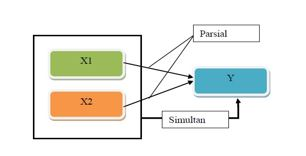
\includegraphics[width=7cm, height=5cm]{figures/modelregresi.JPG}
\caption{\textit{Model Regresi Linier Berganda}
\label{eq:31}}
\end{figure} 
\par Model diatas dapat dijelaskan bahwa dalam model regresi linier berganda mempunyai dua uji pengaruh yaitu :  
\begin{enumerate}
\item 	Pengaruh variabel X (bebas) secara simultan terhadap variabel Y (terikat)  
\item 	Pengaruh variabel X (bebas) secara parsial terhadap variabel Y (terikat), yaitu meliputi:  
\end{enumerate}
    \begin{itemize}
               \item Pengaruh variabel X1 terhadap variabel Y  
               \item Pengaruh variabel X2 terhadap variabel Y 
               \end{itemize}
\section{Tujuan Regresi Linier Berganda}
\begin{enumerate}
\item Untuk membuat perkiraan nilai suatu variabel terikat jika nilai variabel bebas yang berhubungan dengannya sudah ditentukan
\item Untuk menguji hipotesis signifikansi pengaruh dari variabel bebas terhadap variabel terikat
\end{enumerate}

\section{Manfaat Regresi Linier Berganda}
\begin{enumerate}
\item Model regresi dapat digunakan untuk mengukur keeratan hubungan antara variabel dependen (tak bebas) dan variabel independen (bebas). 
\item Model regresi dapat digunakan untuk mengetahui pengaruh suatu atau beberapa variabel independen terhadap variabel dependen (respons).
\item Model regresi dapat digunakan untuk mengetahui pengaruh suatu atau beberapa variabel independen terhadap variabel dependen (respons).
\end{enumerate}

\section{Kelebihan Dan Kekurangan Regresi Linier Berganda}
\par Kelebihan : Dengan menggunakan regresi linear berganda maka dapat menganalisis dengan menggunakan beberapa variabel bebas (X) sehingga hasil prediksi yang didapatkan lebih akurat dibandingkan dengan regresi linear sederhana yang hanya menggunakan satu variabel bebas (X). 
\par Kekurangan : Tidak mampu menunjukkan titik jenuh fungsi yang sedang diselidiki akibatnya selalu timbul kemungkinan kesalahan prediski dan Terdapat kemungkinan terjadinya multikolinearitas pada variabel-variabel bebas. Akibatnya variabel bebas tidak mampu menjelaskan variabel tak bebas (hubungan antara X dan Y tidak bermakna)

\section{Rumus Metode Regresi Linear Berganda}

Analisis regresi linier berganda adalah hubungan secara linear antara dua atau lebih variabel independen (X1, X2) dengan variabel dependen (Y). Analisis ini untuk mengetahui arah hubungan antara variabel independen dengan variabel dependen apakah masing-masing variabel independen berhubungan positif atau negatif dan untuk memprediksi nilai dari variabel dependen apabila nilai variabel independen mengalami kenaikan atau penurunan. Data yang digunakan biasanya berskala interval atau rasio.\citep{smadi2012least}
                        Persamaan regresi linear berganda sebagai berikut:

Y’ = a + b1X1+ b2X2+…..+ bnXn

Keterangan:
Y’                    =   Variabel dependen (nilai yang diprediksikan)
X1 dan X2      =   Variabel independen
a                      =   Konstanta (nilai Y’ apabila X1, X2…..Xn = 0)
b                            =    Koefisien regresi (nilai peningkatan ataupun penurunan)

\newpage \section{Contoh soal Cara Kerja Metode Regresi Linear}
\subsection{Contoh soal 1}
\par Di contoh soal pertama ini penulisa mengambil permasalahan dari kasus di PT Pertamina Gas. Pada kasus di penelitian ini penulis melakukan prediksi \textit{reveniew} dari 5 wilayah milik PT Pertamina Gas. Dan dari setiap wilayah tersebut ada \textit{shipper}(sumber) dan \textit{offtaker}(konsumen)
	Y adalah variabel terikat yang diramalkan (shipper), X adalah variabel bebas. nilai x1(offtaker sinngle) nilai x2 (nilai offtaker multi)\citep{hijriani2017implementasi}
Berikut ini adalah Langkah-langkah dalam melakukan prediksi Regresi Linear Berganda:\citep{analisisrls}
\begin{enumerate}
    \item 	Tentukan nilai a dan b dengan menggunakan SPSS dari 5 wilayah pada PT Pertamina Gas yang di ambil dari data total shipper dan offtaker dari bulan sebelumnya.
     \vspace{9cm}
  \begin{table}[]
  \captionsetup{singlelinecheck=off}
  \caption{\textbf{Eastern Java Area}}
\begin{tabular}{|c|c|c|c|}
\hline
Minggu & Shipper & Single & Multi \\ \hline
1      & 965     & 15     & 308   \\ \hline
2      & 910     & 34     & 616   \\ \hline
3      & 944     & 27     & 616   \\ \hline
4      & 932     & 26     & 637   \\ \hline
5      & 267     & 10     & 183   \\ \hline
\end{tabular}
\end{table}
\newpage \begin{lstlisting}
a= Y-b1X1-b2X2      
a= 325.069
\end{lstlisting}
\begin{figure}[!htbp]
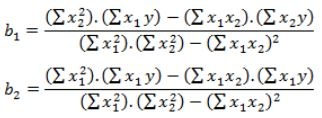
\includegraphics[scale=0.6]{chapters/figures/b1b2.JPG}
    \label{Figure4}
\end{figure}
\begin{lstlisting}
b1= -4.545
b2= 1.23
Rumus:
Y= a+b1X1+b2X2
Y= 325.069+(-4.545x1)+1.23X2
\end{lstlisting}
\vspace{6cm}
\begin{table}[]
  \captionsetup{singlelinecheck=off}
  \caption{\textbf{Kalimantan Area}}
\begin{tabular}{|c|c|c|c|}
\hline
Minggu & Shipper & Single & Multi \\ \hline
1      & 560     & 21     & 378   \\ \hline
2      & 630     & 7     & 378   \\ \hline
3      & 560     & 21     & 378   \\ \hline
4      & 560     & 21     & 378   \\ \hline
5      & 180     & 2     & 108   \\ \hline
\end{tabular}
\end{table}
\newpage \begin{lstlisting}
a= Y-b1X1-b2X2      
a= -0.00000000000014
\end{lstlisting}
\begin{figure}[!htbp]
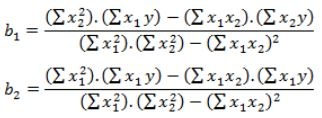
\includegraphics[scale=0.6]{chapters/figures/b1b2.JPG}
    \label{Figure4}
\end{figure}
\begin{lstlisting}
b1= -5
b2= 1.759
Rumus:
Y= a+b1X1+b2X2
Y= -0.00000000000014+(-5x1)+1.759X2
\end{lstlisting}
\vspace{6cm}
\begin{table}[]
  \captionsetup{singlelinecheck=off}
  \caption{\textbf{Northem Sumatra Area}}
\begin{tabular}{|c|c|c|c|}
\hline
Minggu & Shipper & Single & Multi \\ \hline
1      & 597     & 20     & 444   \\ \hline
2      & 646     & 70     & 378   \\ \hline
3      & 737     & 62.01     & 386   \\ \hline
4      & 700     & 70     & 386   \\ \hline
5      & 200     & 20     & 108   \\ \hline
\end{tabular}
\end{table}
\newpage \begin{lstlisting}
a= Y-b1X1-b2X2      
a= 3.319
\end{lstlisting}
\begin{figure}[!htbp]
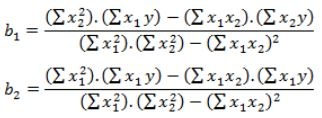
\includegraphics[scale=0.6]{chapters/figures/b1b2.JPG}
    \label{Figure4}
\end{figure}
\begin{lstlisting}
b1= 3.342
b2= 1.207
Rumus:
Y= a+b1X1+b2X2
Y= 3.319+3.342x1+1.207X2
\end{lstlisting}
\vspace{6cm}
\begin{table}[]
  \captionsetup{singlelinecheck=off}
  \caption{\textbf{Southern Sumatra Area}}
\begin{tabular}{|c|c|c|c|}
\hline
Minggu & Shipper & Single & Multi \\ \hline
1      & 640.43     & 9     & 378   \\ \hline
2      & 665.96     & 8     & 378   \\ \hline
3      & 630     & 13     & 378   \\ \hline
4      & 630     & 9     & 378   \\ \hline
5      & 180     & 2     & 108   \\ \hline
\end{tabular}
\end{table}
\newpage \begin{lstlisting}
a= Y-b1X1-b2X2      
a= -9.915
\end{lstlisting}
\begin{figure}[!htbp]
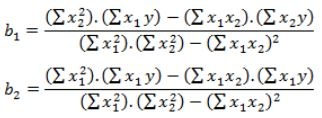
\includegraphics[scale=0.6]{chapters/figures/b1b2.JPG}
    \label{Figure4}
\end{figure}
\begin{lstlisting}
b1= -4.797
b2= 1.847
Rumus:
Y= a+b1X1+b2X2
Y= -9.915+(-4.797x1)+1.847X2
\end{lstlisting}
\vspace{6cm}
\begin{table}[]
  \captionsetup{singlelinecheck=off}
  \caption{\textbf{Western Java Area}}
\begin{tabular}{|c|c|c|c|}
\hline
Minggu & Shipper & Single & Multi \\ \hline
1      & 630     & 14    & 315   \\ \hline
2      & 700     & 14    & 313   \\ \hline
3      & 700     & 14     & 308   \\ \hline
4      & 700     & 14     & 353   \\ \hline
5      & 200     & 4     & 133   \\ \hline
\end{tabular}
\end{table}
\newpage \begin{lstlisting}
a= Y-b1X1-b2X2      
a= -15.599
\end{lstlisting}
\begin{figure}[!htbp]
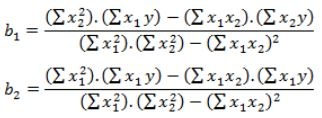
\includegraphics[scale=0.6]{chapters/figures/b1b2.JPG}
    \label{Figure4}
\end{figure}
\begin{lstlisting}
b1= 40.786
b2= 0.394
Rumus:
Y= a+b1X1+b2X2
Y= -15.599+40.786x1+0.394X2
\end{lstlisting}
\newpage \item Setelah itu masukkan ke rumus untuk memprediksi nilai Y(shipper). Y= a+b1X1+b2X2
\item Setelah nilai Y di temukan di kurangkan kembali dengan nilai total perminggu offtaker single dan multi untuk mengetahui sisa shipper.
\item Setelah di temukan nilai total pendapatan perminggu kemudian di jumlahkan untuk mengetahui total pendapatan perbulan
\item Untuk mengetahui reveniew nya total perbulan di akumulasikan ke dollar (perkalian 1MSCF= 4 US dollar).

\end{enumerate}
 \par Berikut adalah hasil perhitungan regresi dan prediksi dalam kalkulasi \$ di bulan berikutnya:
\begin{figure}[!htbp]
    \centering
    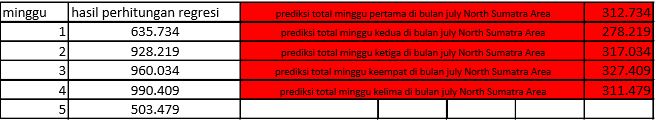
\includegraphics[scale=0.7]{chapters/figures/11.JPG}
\end{figure}
\begin{figure}[!htbp]
    \centering
    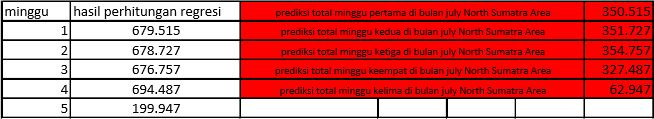
\includegraphics[scale=0.7]{chapters/figures/22.JPG}
\end{figure}
\begin{figure}[!htbp]
    \centering
    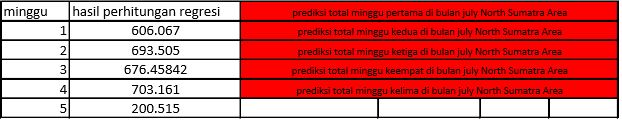
\includegraphics[scale=0.7]{chapters/figures/33.JPG}
\end{figure}
\begin{figure}[!htbp]
    \centering
    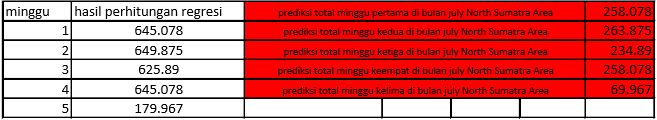
\includegraphics[scale=0.7]{chapters/figures/44.JPG}
\end{figure}
\begin{figure}[!htbp]
    \centering
    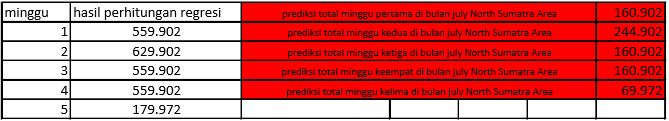
\includegraphics[scale=0.7]{chapters/figures/55.JPG}
\end{figure}
\newpage  \subsection{Contoh soal 2}
\par Kita mengambil contoh kasus pada uji normalitas, yaitu sebagai berikut: Seorang mahasiswa bernama Bambang melakukan penelitian tentang faktor-faktor yang mempengaruhi harga saham pada perusahaan di BEJ.\citep{priyatno2014spss} Bambang dalam penelitiannya ingin mengetahui hubungan antara rasio keuangan PER dan ROI terhadap harga saham. Dengan ini Bambang menganalisis dengan bantuan program SPSS dengan alat analisis regresi linear berganda. Dari uraian di atas maka didapat variabel dependen (Y) adalah harga saham, sedangkan variabel independen (X1 dan X2) adalah PER dan ROI.
Data-data yang di dapat berupa data rasio dan ditabulasikan sebagai berikut: \begin{figure}[!htbp]
    \centering
    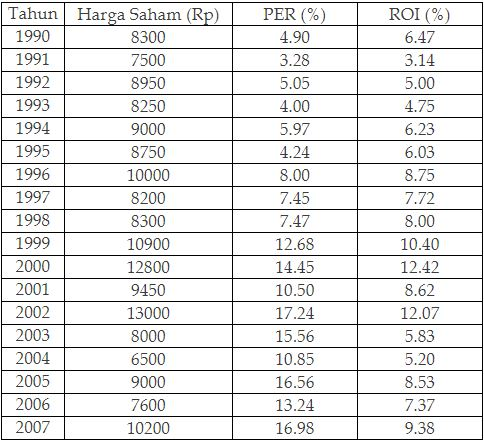
\includegraphics[scale=0.7]{chapters/figures/cs.JPG}
    \caption{Tabulasi Data (Data Fiktif)}
\end{figure}
\newpage \par Langkah berikutnya sama dengan langkah di contoh soal 1. Mencari nilai a dan b nya. \begin{lstlisting}
a= Y-b1X1-b2X2      
a= 4662.491
\end{lstlisting}
\begin{figure}[!htbp]
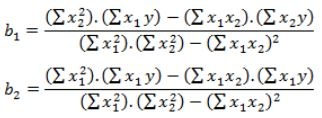
\includegraphics[scale=0.6]{chapters/figures/b1b2.JPG}
    \label{Figure4}
\end{figure}
\begin{lstlisting}
b1= -74.482
b2= 692.107
\end{lstlisting}
Setelah variabel a dan b di temukan maka di masukkan ke dalam rumus seperti berikut: 
Persamaan regresinya sebagai berikut:
\begin{lstlisting}
Y’ = a + b1X1+ b2X2
Y’ =  4662,491 + (-74,482)X1 + 692,107X2
Y’ =  4662,491 - 74,482X1 + 692,107X2
\end{lstlisting}
Keterangan:
\begin{lstlisting}
Y’        = Harga saham yang diprediksi (Rp)
a          = konstanta
b1,b2    = koefisien regresi
X1        = PER (\%)
X2        = ROI (\%)
\end{lstlisting}
\par Langkah berikutnya adalah memasukkan nilai x1(PER (\%)) dan x2(ROI (\%)) ke dalam rumus, sehingga di temukan hasil prediksi sebagai berikut:
\begin{figure}[!htbp]
    \centering
    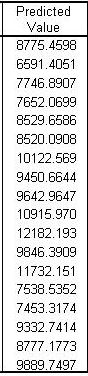
\includegraphics[scale=0.6]{chapters/figures/cs3.JPG}
    \caption{Hasil Perhitungan Prediksi}
\end{figure}
\newpage \subsection{Contoh soal 3}
\par Di contoh soal 3 ini kita akan menghitung data pengeluaran 10 rumah tangga, untuk pembelian barang tahan lama per minggu(Y), pendapatan per minggu (X1), dan jumlah anggota keluarga (X2).
\par Berikut adalah data mentahan nya:
\begin{figure}[!htbp]
    \centering
    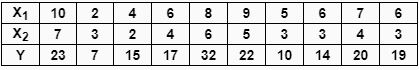
\includegraphics[scale=0.7]{chapters/figures/css.JPG}
    \caption{Data mentahan}
\end{figure}




\chapter{KLASIFIKASI}
\pagebreak
\section{\textit{K Nearest Neighbor}}
\subsection{Pengertian \textit{K Nearest Neighbor}}
\textit{K Nearest Neighbor} atau biasa disebut dengan KNN merupakan salah satu algoritma \textit{supervised learning}, dimana \textit{supervised learning} merupakan sebuah teknik pendekatan dengan sudah terdapat data latih, variabel yang ditargetkan dengan tujuan mengelompokkan suatu data ke data yang sudah ada. KNN biasanya digunakan untuk melakukan proses klasifikasi sebuah obyek/data baru dengan berdasarkan pada atribut dan sampel \textit{training}, dan berdasarkan kedekatan jarak antara data yang akan dievaluasi dengan k (tetangga/\textit{neighbor}) pada data latih (\textit{training})\cite{hermaduanti2008sistem}.

\subsection{Kelebihan dan Kekurangan \textit{K Nearest Neighbor}}
\begin{enumerate}
    \item Kelebihan
\begin{itemize}
        \item Sangat sederhana implementasi.
        \item Kuat dalam hal ruang pencarian, misalnya, kelas tidak harus linear dipisahkan.
        \item Sangat Non Linear
        \par KNN merupakan salah satu algoritma yang bersifat non parametrik, yang artinya tidak mengasumsikan tentang distribusi dari \textit{isntance} pada \textit{dataset}. Model ini memiliki kelebihan pada model yang dihasilkan yaitu berdifat fleksibel dan non linear.
        \begin{figure}[!htpb]
        \centering
        \includegraphics[width=6cm, height=4cm]{figureshanna/Knn.jpg}
        \caption{Non Linear
        \label{eq:31}}
        \end{figure} 
        \item Efektif untuk menghitung data dalam skala kecil.
        \item Beberapa parameter untuk acuan : jarak metrik dan k \cite{lestari2015penerapan}.
\end{itemize}
\item Kekurangan
    \begin{itemize}
        \item Perlu untuk menentukan nilai k yang optimal sehingga untuk menyatakan jumlah
tatangga terdekatnya lebih mudah.
        \item  Biaya komputasi yang cukup tinggi karena perhitungan jarak harus dilakukan pada setiap \textit{querry instance}\cite{afandie2014implementasi}.
    \end{itemize}
\end{enumerate}
\subsection{Langkah-langkah dalam Klasifikasi \textit{K Nearest Neighbor}}
\begin{enumerate}
    \item Tentukan parameter K (jumlah tetangga paling dekat).
    \item Hitung kuadrat jarak euclid masing – masing objek terhadap data sample yang
diberikan. Rumus yang digunakan adalah sebagai berikut:
    \begin{equation}
        D(a,b)= \sqrt{\sum_{k=1}^{d}(a_{k}-b_{k})^{2}}
        \label{rumusknn1}
    \end{equation}
    \par Dimana D(a,b) merupakan jarak skalar dari dua buah vektor antara data a dan data b yang berbentuk matrik dengan ukuran d dimensi.
    \item Urutkan objek – objek kedalam kelompok yang memiliki jarak terkecil.
    \item Kumpulkan kategori Y (Klasifikasi nearest neighbor).
    \item Dengan kategori nearest neighbor yang paling banyak, maka dapat diprediksikan
nilai query instance yang telah dihitung\cite{zainuddin2019implementasi}.
\end{enumerate}

Berikut merupakan penerapan contoh perhitungan K-Nearest Neighbor pada contoh soal untuk menentukan kelas Baik atau Buruk. Pada tabel \ref{knn1} merupakan data \textit{training} yang akan digunakan.
\begin{table}[!ht]
\centering
\caption{Contoh Data \textit{Training} pada KNN}
\label{knn1}
\begin{tabular}{|l|l|l|}
\hline
A1 & A2 & Y     \\ \hline
7  & 7  & BURUK \\ \hline
7  & 4  & BURUK \\ \hline
3  & 4  & BAIK  \\ \hline
1  & 4  & BAIK  \\ \hline
\end{tabular}
\end{table}
Diketahui sebuah data yang akan dicari hasil klasifikasinya, perhatikan pada tabel \ref{knn2}.
\begin{table}[!ht]
\centering
\caption{Contoh Data \textit{Testing} KNN}
\label{knn2}
\begin{tabular}{|l|l|l|}
\hline
A1 & A2 & Y   \\ \hline
3  & 7  & ..? \\ \hline
\end{tabular}
\end{table}
Ikuti langkah-langkah yang sebelumnya sudah dijelaskan, yakni sebagai berikut:
\begin{enumerate}
    \item Tentukan parameter k (jumlah tetangga terdekat), misal k=3
    \item Hitung jarak antara data baru dengan semua data \textit{training} mengggunakan rumus \ref{rumusknn1}, Perhatikan tabel \ref{knn3}.
    \begin{table}[!ht]
    \centering
    \caption{Jarak Eucliden}
    \label{knn3}
\begin{tabular}{|l|l|l|}
\hline
A1 & A2 & Eucliden(3,7)               \\ \hline
7  & 7  & (7-3)$^{2}$ + (7-7)$^{2}$= 16 \\ \hline
7  & 4  & (7-3)$^{2}$ + (4-7)$^{2}$= 25 \\ \hline
3  & 4  & (3-3)$^{2}$ + (4-7)$^{2}$= 9 \\ \hline
1  & 4  & (1-3)$^{2}$ + (4-7)$^{2}$= 13 \\ \hline
\end{tabular}
\end{table}
\item Setelah diperoleh nilai \textit{Eucliden}, kemudian urutkan nilai jarak tersebut dan tetapkan tetangga yang terdekat berdasarkan dengan jarak minimum ke k
\begin{table}[!ht]
    \centering
    \caption{Rank Jarak}
    \label{knn3}
\begin{tabular}{|l|l|l|l|l|}
\hline
A1 & A2 & Eucliden(3,7)               & Rank & 3 tetangga terdekat? \\ \hline
7  & 7  & (7-3)$^{2}$ + (7-7)$^{2}$= 16 & 3    & Ya                   \\ \hline
7  & 4  & (7-3)$^{2}$ + (4-7)$^{2}$= 25 & 4    & Tidak                \\ \hline
3  & 4  & (3-3)$^{2}$ + (4-7)$^{2}$= 9  & 1    & Ya                   \\ \hline
1  & 4  & (1-3)$^{2}$ + (4-7)$^{2}$= 13 & 2    & Ya                   \\ \hline
\end{tabular}
\end{table}
\pagebreak
\item Kemudian perhatikan kelas dari tetangga tersebut, nilai klasifikasi yang paling banyak pada tetangga terdekat merupakan hasil klasifikasi dari data \textit{testing}
\begin{table}[!ht]
    \centering
    \caption{Hasil Klasifikasi}
    \label{knn3}
\begin{tabular}{|l|l|l|l|l|l|}
\hline
A1 & A2 & Eucliden(3,7)               & Rank & 3 tetangga terdekat? & Y             \\ \hline
7  & 7  & (7-3)$^{2}$ + (7-7)$^{2}$= 16 & 3    & Ya                   & Buruk         \\ \hline
7  & 4  & (7-3)$^{2}$ + (4-7)$^{2}$= 25 & 4    & Tidak                & -             \\ \hline
3  & 4  & (3-3)$^{2}$ + (4-7)$^{2}$= 9  & 1    & Ya                   & \textbf{Baik} \\ \hline
1  & 4  & (1-3)$^{2}$ + (4-7)$^{2}$= 13 & 2    & Ya                   & \textbf{Baik} \\ \hline
\end{tabular}
\end{table}
\end{enumerate}
Maka dapat disimpulkan bahwa data dengan nilai A1=3 dan A2=7 memiliki hasil klasifikasi \textbf{baik}.

\subsection{Soal Latihan}
\begin{enumerate}
    \item Sebuah rumah tepat berada di antara kota dan kabupaten, pemerintah bingung menentukan posisi rumah apakah termasuk ke dalam daerah kota atau kabupatan. Tentukan posisi rumah berada di daerah mana?
    \begin{table}[!htpb]
    \centering
\begin{tabular}{|l|l|l|l|}
\hline
Rumah & Langitude & Longitude & Lokasi    \\ \hline
A     & 11        & 26        & Kota      \\ \hline
B     & 15        & 29        & Kota      \\ \hline
C     & 19        & 28        & Kota      \\ \hline
D     & 18        & 30        & Kota      \\ \hline
E     & 16        & 26        & Kota      \\ \hline
F     & 23        & 25        & Kabupaten \\ \hline
G     & 25        & 22        & Kabupaten \\ \hline
H     & 21        & 24        & Kabupaten \\ \hline
I     & 29        & 24        & Kabupaten \\ \hline
Z     & 19        & 25        & .....?    \\ \hline
\end{tabular}
\end{table}
\end{enumerate}
\pagebreak
\section{\textit{Naive Bayes Classifier}}
\subsection{Pengertian \textit{Naive Bayes Classifier}}
\textit{Naive Bayes Classifier} merupakan salah satu metode klasifikasi probabilistik dan statistik yang dikemukakan oleh Thomas Bayes. Algoritma \textit{Naive Bayes} biasa digunakan untuk memprediksi peluang di masa depan  berdasarkan pengalaman di masa sebelumnya (Teorema \textit{Bayes}) dengan asumsi independensi (ketidaktergantungan) yang kuat (naif)\cite{saleh2015implementasi}.
\subsection{Kelebihan dan Kekurangan \textit{Naive Bayes}}
\begin{enumerate}
    \item Kelebihan
    \begin{itemize}
        \item Dapat menangani data kuantitatif dan data diskrit.
        \item Dapat menggunakan sedikit data \textit{training} untuk pengestimasian parameter yang dibutuhkan untuk klasifikasi.
        \item Lebih Cepat dan Efisien \cite{hidayat2018klasifikasi}.
    \end{itemize}
    \item Kekurangan
    \begin{itemize}
        \item Tidak berlaku apabila memiliki nilai probabilitas 0 (nol), sehingga prediksi juga bernilai nol.
        \item Asumsi variabel yang bebas\cite{akbar2017prediksi}.
    \end{itemize}
\end{enumerate}
Persamaan dari teorema \textit{Bayes} adalah:
\begin{equation}
P(H|X) = \frac{P(X|H)P(H)}{P(X)} \\
\end{equation}
Keterangan : 
\par X 		: Data dengan class yang belum diketahui 
\par H 		: Hipotesis data merupakan suatu class spesifik 
\par P(H|X) 	: Probabilitas hipotesis H berdasar kondisi X (posteriori       probabilitas) 
\par P(H) 		: Probabilitas hipotesis H (prior probabilitas) 
\par P(X|H) 	: Probabilitas X berdasarkan kondisi pada hipotesis H 
\par P(X) 	: Probabilitas X 
\par Persamaan \textit{Naive Bayes} adalah:
\begin{equation}
    P(X|C_{i})=\prod_{k=1}^{n}P(x_{k}|C_{i})
    \label{rumus2}
\end{equation}
\subsection{Langkah-langkah dalam Klasifikasi \textit{Naive Bayes}}
Dalam melakukan klasifikasi \textit{Naive Bayes} berikut tahapan-tahapan yang harus dilakukan \cite{kosasih2018pengklasifikasian}:
Berikut adalah contoh data yang akan digunakan, perhatikan pada tabel \ref{contohdata}.
\begin{table}[!ht]
\centering
\caption{Contoh Data \textit{Training}}
\label{contohdata}
\begin{tabular}{|l|l|l|l|l|}
\hline
Umur             & Pendapatan & Mhs   & Rating Kredit & Beli Komputer \\ \hline
\textless{}=30   & tinggi     & bukan & fair          & tdk           \\ \hline
\textless{}=30   & tinggi     & bukan & excellent     & tdk           \\ \hline
30…40            & tinggi     & bukan & fair          & ya            \\ \hline
\textgreater{}40 & sedang     & bukan & fair          & ya            \\ \hline
\textgreater{}40 & rendah     & ya    & fair          & ya            \\ \hline
\textgreater{}40 & rendah     & ya    & excellent     & tdk           \\ \hline
31…40            & rendah     & ya    & excellent     & ya            \\ \hline
\textless{}=30   & sedang     & bukan & fair          & tdk           \\ \hline
\textless{}=30   & rendah     & ya    & fair          & ya            \\ \hline
\textgreater{}40 & sedang     & ya    & fair          & ya            \\ \hline
\textless{}=30   & sedang     & ya    & excellent     & ya            \\ \hline
31…40            & sedang     & bukan & excellent     & ya            \\ \hline
31…40            & tinggi     & ya    & fair          & ya            \\ \hline
\textgreater{}40 & sedang     & bukan & excellent     & tdk           \\ \hline
\end{tabular}
\end{table}
Misalkan ada sebuah data \textit{testing} yang ingin diketahui masuk ke dalam hasil klasifikasi mana, berikut contoh data \textit{testing} yang akan digunakan, perhatikan pada tabel \ref{testing}
\begin{table}[!ht]
\centering
\caption{Contoh Data \textit{Testing}}
\label{testing}
\begin{tabular}{|l|l|l|l|l|}
\hline
Umur           & Pendapatan & Mhs & Rating Kredit & Beli Komputer \\ \hline
\textless{}=30 & sedang     & ya  & fair          & ...?          \\ \hline
\end{tabular}
\end{table}
\par Langkah selanjutnya, dengan menghitung nilai $P(X_{k}|C_{i})$ pada setiap \textit{class}.

\begin{enumerate}
    \item $P(umur :\textless{}=30|Beli Komputer)$
    \par Perhatikan pada tabel \ref{prob1} pada kolom Umur, diperoleh bahwa probabilitas Umur dengan $\textless{}=30$ terhadap kelas beli komputer dengan nilai ya adalah sebanyak 2 data, dan untuk kelas beli komputer dengan nilai tidak sebanyak 3 data. Nilai probabilitasnya yakni sebagai berikut:
\par $P(umur :\textless{}=30|Beli Komputer:Ya)$ = 2/9 = 0.220
\par $P(umur :\textless{}=30|Beli Komputer:Tidak)$ = 3/5 = 0.600
\par nilai 9 merupakan jumlah data dengan kelas Ya sebanyak 9, dan nilai 5 merupakan jumlah data dengan kelas Tidak sebanyak 5.
\item $P(pendapatan :sedang|Beli Komputer)$
\par Perhatikan pada tabel \ref{prob2} pada kolom Pendapatan, diperoleh bahwa probabilitas Umur dengan $\textless{}=30$ terhadap kelas beli komputer dengan nilai ya adalah sebanyak 4 data, dan untuk kelas beli komputer dengan nilai tidak sebanyak 2 data. Nilai probabilitasnya yakni sebagai berikut:
\par $P(pendapatan :sedang|Beli Komputer:Ya)$ = 4/9= 0.444
\par $P(pendapatan :sedang|Beli Komputer:Tidak)$ = 2/5=0.400

\item $P(Mhs:ya|Beli Komputer)$
\par Perhatikan pada tabel \ref{prob2} pada kolom Mhs, diperoleh bahwa probabilitas Umur dengan $\textless{}=30$ terhadap kelas beli komputer dengan nilai ya adalah sebanyak 6 data, dan untuk kelas beli komputer dengan nilai tidak sebanyak 1 data. Nilai probabilitasnya yakni sebagai berikut:
\par $P(Mhs:ya|Beli Komputer:Ya)$ = 6/9 =  0.670 
\par $P(Mhs:ya|Beli Komputer:Tidak)$ = 1/5	 =  0.200

\item $P(Ratingkredit:Fair|Beli Komputer)$
\par Perhatikan pada tabel \ref{prob2} pada kolom Rating Kredit, diperoleh bahwa probabilitas Umur dengan $\textless{}=30$ terhadap kelas beli komputer dengan nilai ya adalah sebanyak 6 data, dan untuk kelas beli komputer dengan nilai tidak sebanyak 2 data. Nilai probabilitasnya yakni sebagai berikut:
\par $P(Ratingkredit:Fair|Beli Komputer:Ya)$ = 6/9	=  0.670
\par $P(Ratingkredit:Fair|Beli Komputer:Tidak)$ = 2/5  =  0.400
    \begin{table}[!ht]
    \centering
    \caption{Hitung Nilai Probabilitas $P(umur :\textless{}=30|Beli Komputer)$ }
    \label{prob1}
\begin{tabular}{|l|l|l|l|l|}
\hline
\textbf{Umur}             & Pendapatan & Mhs   & Rating Kredit & Beli Komputer \\ \hline
\textbf{\textless{}=30}   & tinggi     & bukan & fair          & tdk           \\ \hline
\textbf{\textless{}=30}   & tinggi     & bukan & excellent     & tdk           \\ \hline
\textbf{\textless{}=30}   & sedang     & bukan & fair          & tdk           \\ \hline
\textbf{\textless{}=30}   & rendah     & ya    & fair          & ya            \\ \hline
\textbf{\textless{}=30}   & sedang     & ya    & excellent     & ya            \\ \hline
\textbf{\textgreater{}40} & rendah     & ya    & excellent     & tdk           \\ \hline
\textbf{\textgreater{}40} & sedang     & bukan & fair          & ya            \\ \hline
\textbf{\textgreater{}40} & rendah     & ya    & fair          & ya            \\ \hline
\textbf{\textgreater{}40} & sedang     & ya    & fair          & ya            \\ \hline
\textbf{\textgreater{}40} & sedang     & bukan & excellent     & tdk           \\ \hline
\textbf{30…40}            & tinggi     & bukan & fair          & ya            \\ \hline
\textbf{31…40}            & rendah     & ya    & excellent     & ya            \\ \hline
\textbf{31…40}            & sedang     & bukan & excellent     & ya            \\ \hline
\textbf{31…40}            & tinggi     & ya    & fair          & ya            \\ \hline
\end{tabular}
\end{table}



\begin{table}[!ht]
\centering
\caption{Hitung Nilai Probabilitas $P(pendapatan :sedang|Beli Komputer)$ }
\label{prob2}
\begin{tabular}{|l|l|l|l|l|}
\hline
Umur             & \textbf{Pendapatan} & Mhs   & Rating Kredit & Beli Komputer \\ \hline
\textgreater{}40 & \textbf{rendah}     & ya    & excellent     & tdk           \\ \hline
\textless{}=30   & \textbf{rendah}     & ya    & fair          & ya            \\ \hline
\textgreater{}40 & \textbf{rendah}     & ya    & fair          & ya            \\ \hline
31…40            & \textbf{rendah}     & ya    & excellent     & ya            \\ \hline
\textless{}=30   & \textbf{sedang}     & bukan & fair          & tdk           \\ \hline
\textgreater{}40 & \textbf{sedang}     & bukan & excellent     & tdk           \\ \hline
\textless{}=30   & \textbf{sedang}     & ya    & excellent     & ya            \\ \hline
\textgreater{}40 & \textbf{sedang}     & bukan & fair          & ya            \\ \hline
\textgreater{}40 & \textbf{sedang}     & ya    & fair          & ya            \\ \hline
31…40            & \textbf{sedang}     & bukan & excellent     & ya            \\ \hline
\textless{}=30   & \textbf{tinggi}     & bukan & fair          & tdk           \\ \hline
\textless{}=30   & \textbf{tinggi}     & bukan & excellent     & tdk           \\ \hline
30…40            & \textbf{tinggi}     & bukan & fair          & ya            \\ \hline
31…40            & \textbf{tinggi}     & ya    & fair          & ya            \\ \hline
\end{tabular}
\end{table}


\begin{table}[!ht]
\centering
\caption{Hitung Nilai Probabilitas $P(Mhs:ya|Beli Komputer)$ }
\label{prob2}
\begin{tabular}{|l|l|l|l|l|}
\hline
Umur             & Pendapatan & \textbf{Mhs}   & Rating Kredit & Beli Komputer \\ \hline
\textless{}=30   & sedang     & \textbf{bukan} & fair          & tdk           \\ \hline
\textgreater{}40 & sedang     & \textbf{bukan} & excellent     & tdk           \\ \hline
\textless{}=30   & tinggi     & \textbf{bukan} & fair          & tdk           \\ \hline
\textless{}=30   & tinggi     & \textbf{bukan} & excellent     & tdk           \\ \hline
\textgreater{}40 & sedang     & \textbf{bukan} & fair          & ya            \\ \hline
31…40            & sedang     & \textbf{bukan} & excellent     & ya            \\ \hline
30…40            & tinggi     & \textbf{bukan} & fair          & ya            \\ \hline
\textgreater{}40 & rendah     & \textbf{ya}    & excellent     & tdk           \\ \hline
\textless{}=30   & rendah     & \textbf{ya}    & fair          & ya            \\ \hline
\textgreater{}40 & rendah     & \textbf{ya}    & fair          & ya            \\ \hline
31…40            & rendah     & \textbf{ya}    & excellent     & ya            \\ \hline
\textless{}=30   & sedang     & \textbf{ya}    & excellent     & ya            \\ \hline
\textgreater{}40 & sedang     & \textbf{ya}    & fair          & ya            \\ \hline
31…40            & tinggi     & \textbf{ya}    & fair          & ya            \\ \hline
\end{tabular}
\end{table}



\begin{table}[!ht]
\centering
\caption{Hitung Nilai Probabilitas $P(Ratingkredit:Fair|Beli Komputer)$}
\label{prob2}
\begin{tabular}{|l|l|l|l|l|}
\hline
Umur             & Pendapatan & Mhs   & \textbf{Rating Kredit} & Beli Komputer \\ \hline
\textless{}=30   & tinggi     & bukan & \textbf{excellent}     & tdk           \\ \hline
\textgreater{}40 & sedang     & bukan & \textbf{excellent}     & tdk           \\ \hline
\textgreater{}40 & rendah     & ya    & \textbf{excellent}     & tdk           \\ \hline
31…40            & sedang     & bukan & \textbf{excellent}     & ya            \\ \hline
31…40            & rendah     & ya    & \textbf{excellent}     & ya            \\ \hline
\textless{}=30   & sedang     & ya    & \textbf{excellent}     & ya            \\ \hline
\textless{}=30   & sedang     & bukan & \textbf{fair}          & tdk           \\ \hline
\textless{}=30   & tinggi     & bukan & \textbf{fair}          & tdk           \\ \hline
\textgreater{}40 & sedang     & bukan & \textbf{fair}          & ya            \\ \hline
30…40            & tinggi     & bukan & \textbf{fair}          & ya            \\ \hline
\textless{}=30   & rendah     & ya    & \textbf{fair}          & ya            \\ \hline
\textgreater{}40 & rendah     & ya    & \textbf{fair}          & ya            \\ \hline
\textgreater{}40 & sedang     & ya    & \textbf{fair}          & ya            \\ \hline
31…40            & tinggi     & ya    & \textbf{fair}          & ya            \\ \hline
\end{tabular}
\end{table}
\pagebreak
\pagebreak
\par Setelah dihitung nilai  $P(X_{k}|C_{i})$, maka tahap selanjutnya menghitung nilai probabilitas kelas yang diperoleh setelah melakukan perhitungan probabilitas atribut terhadap kelas, berikut hasil perhitungannya pada table \ref{hasil1}
\begin{table}[!ht]
\centering
\caption{Hitung nilai probabilitas}
\label{hasil1}
\begin{tabular}{|l|l|}
\hline
\multicolumn{2}{|c|}{\begin{tabular}[c]{@{}c@{}}Hitung P(Xk | Ci)\\   utk setiap class I\end{tabular}} \\ \hline
P(umur\textless{}=30|beli\_komputer=ya)           = 2/9                    & 0.222                    \\ \hline
P(umur\textless{}=30|beli\_komputer=tdk)         = 3/5                      & 0.6                      \\ \hline
P(pendapatan=sedang|beli\_komputer=ya)      = 4/9                           & 0.444                    \\ \hline
P(pendapatan=sedang|beli\_komputer=tdk)     = 2/5                           & 0.4                      \\ \hline
P(mhs=ya|beli\_komputer=ya)      = 6/9                                      & 0.667                    \\ \hline
P(mhs=ya| beli\_komputer=tdk)     = 1/5                                     & 0.2                      \\ \hline
P(ratingkredit=fair| beli\_komputer=ya)      =6/9                           & 0.667                    \\ \hline
P(rating kredit=ya|beli\_komputer=tdk)     = 2/5                            & 0.4                      \\ \hline
\end{tabular}
\end{table}

\par Setelah diperoleh nilai probabilitas kelas, kemudian kalikan nilai probabilitas yang diperoleh terhadap nilai probabilitas kelas, berikut peehitungannya:
\par P(X|belicomputer=“ya”) * P(belicomputer=“ya”) = 0.044*(9/14) = 0.028
\par P(X|belicomputer=“tidak”) * P(belicomputer=“tidak”) = 0.044*(5/14)= 0.007

\par Setelah mengalikan nilai probabilitas,maka diperoleh hasil bahwa data sesuai pada tabel \ref{tab2} diklasifikasikan pada \textbf{Ya}, karena nilai probabilitas lebih besar dari pengujian yang lain.   

\end{enumerate}
\subsection{Soal Latihan}
\begin{enumerate}
    \item Kerjakan soal dibawah ini, tentukan \textit{class label} dari data dibawah ini, 
    \begin{table}[!ht]
    \centering
\begin{tabular}{|l|l|l|l|l|l|l|l|l|}
\hline
No & Nama                & A1 & A2 & A3 & A4 & A5 & A6 & Hasil \\ \hline
1  & Yoka Alit Kameswara & 2  & 4  & 3  & 2  & 3  & 6  & ....? \\ \hline
\end{tabular}
\end{table}
berikut penjelasan tentang atribut yang digunakan pada soal ini, perhatikan tabel \ref{soal1}
    \begin{table}[!ht]
    \centering
    \caption{Penjelasan Atribut Soal}
    \label{soal1}
\begin{tabular}{|l|l|l|l|l|}
\hline
No & Atribute                      & Nilai            & Label & Keterangan  \\ \hline
1  & Usia (A1)                     & Sangat Produktif & 3     & 15-49 tahun \\ \hline
   &                               & Produktif        & 2     & 50-64 tahun \\ \hline
   &                               & Tidak produktif  & 1     & 65 tahun    \\ \hline
2  & Pendidikan (A2)               & PT               & 4     &             \\ \hline
   &                               & SMA              & 3     &             \\ \hline
   &                               & SMP              & 2     &             \\ \hline
   &                               & SD               & 1     &             \\ \hline
3  & Pekerjaan (A3)                & Tetap            & 3     &             \\ \hline
   &                               & Tidak tetap      & 2     &             \\ \hline
   &                               & Tidak bekerja    & 1     &             \\ \hline
4  & Tanggungan (A4)               & \textless{}4     & 2     &             \\ \hline
   &                               & \textgreater{}4  & 1     &             \\ \hline
5  & Status kepemilikan Rumah (A5) & Milik sendiri    & 3     &             \\ \hline
   &                               & Sewa/Kontrak     & 2     &             \\ \hline
   &                               & Menumpang        & 1     &             \\ \hline
6  & Luas Rumah (A6)               & Tipe 120         & 6     &             \\ \hline
   &                               & Tipe 60          & 5     &             \\ \hline
   &                               & Tipe 54          & 4     &             \\ \hline
   &                               & Tipe 45          & 3     &             \\ \hline
   &                               & Tipe 36          & 2     &             \\ \hline
   &                               & Tipe 21          & 1     &             \\ \hline
\end{tabular}
\end{table}
    \begin{table}[!ht]
    \centering
\begin{tabular}{|l|l|l|l|l|l|l|l|l|}
\hline
No & Nama             & A1 & A2 & A3 & A4 & A5 & A6 & Hasil         \\ \hline
1  & Usep Heliana     & 3  & 2  & 3  & 2  & 1  & 6  & Pra Sejahtera \\ \hline
2  & A Rahmat         & 2  & 1  & 2  & 2  & 1  & 6  & Pra Sejahtera \\ \hline
3  & Ujang Tarman     & 3  & 1  & 3  & 2  & 3  & 6  & Sejahtera 1   \\ \hline
4  & Maimunah         & 3  & 3  & 1  & 2  & 1  & 6  & Pra Sejahtera \\ \hline
5  & Kasna            & 2  & 1  & 3  & 2  & 3  & 6  & Sejahtera 1   \\ \hline
6  & Wiwi             & 2  & 1  & 2  & 2  & 3  & 6  & Sejahtera 1   \\ \hline
7  & Mufti Handoko    & 3  & 4  & 3  & 2  & 3  & 6  & Sejahtera 2   \\ \hline
8  & Atam             & 1  & 3  & 3  & 2  & 3  & 6  & Sejahtera 1   \\ \hline
9  & Entis Sutisna    & 3  & 2  & 3  & 2  & 3  & 6  & Sejahtera 2   \\ \hline
10 & Jajang Supriatna & 3  & 3  & 3  & 2  & 3  & 6  & Sejahtera 2   \\ \hline
\end{tabular}
\end{table}
\end{enumerate}

\section{Algoritma Apriori}
\subsection{Pengertian Algoritma Apriori}
Algoritma apriori merupakan jenis aturan asosiasi pada data mining, dimana aturan yang menyatakan asosiasi antara atribut-atribut yang disebut \textit{market basket analysis} \cite{ye2006parallel}. \textit{Asosiation rule} adalah teknik data minig yang digunakan untuk menentukan atura asosiatif antar suatu kombinasi \textit{item}. Algoritma apriori yang bertujuan untuk menemukan \textit{frequent itemsets} pada sekumpulan data yang memenuhi syarat minimum \textit{support} dan minimum \textit{confidence} yang telah ditentukan.
\par
Algoritma Apriori menggunakan pengetahuan frekuensi atribut yang  sebelumnya telah didapat untuk dilakukan proses informasi selanjutnya. Pada algoritma Apriori  menentukan kandidat yang mungkin muncul dengan cara memperhatikan nilai minimum \textit{support} dan nilai minimum \textit{confidence}. \textit{Support} adalah nilai pengunjung atau persentase kombinasi sebuah \textit{item} dalam \textit{database}. Sedangkan \textit{confidence} adalah nilai kepastian yang menentukan kuatnya hubungan antar \textit{item} dalam sebuah Apriori. \textit{Confidence} dapat dicari setelah pola frekuensi munculnya sebuah \textit{item} ditemukan.


\subsection{Kelebihan dan Kelemahan Algoritma Apriori}
\par Beberapa kelebihan yang dimiliki oleh algoritma apriori adalah sebagai berikut \cite{fauzy2016penerapan}:
 \begin{enumerate}
\item Menghasilkan kombinasi yang sangat banyak sehingga sangat tidak efisien. 
\item Lebih sederhana
\item Dapat menangani data yang besar
\item Apriori memiliki akurasi rules yang tinggi
\end{enumerate}

\par Beberapa kelemahan yang dimiliki oleh algoritma apriori adalah sebagai berikut:
 \begin{enumerate}
\item Proses \textit{scan database} yang dilakukan setiap kali iterasi, sehingga waktu yang diperlukan bertambah dengan makin banyak iterasi
\item Proses \textit{scanning} yang
dilakukan pada apriori yang berulang kali membuat tingkat kecepatan menjadi lambat

\end{enumerate}

\subsection{Tahap-Tahap Menghitung Algoritma Apriori}
Tahap-tahap yang dilakukan untuk mendapatkan \textit{frequent itemset} dalam algoritma apriori adalah sebagai berikut \cite{triyanto2014association}:
 \begin{enumerate}
\item Penggabungan (\textit{Join})
\par Proses penggabungan dilakukan dengan melakukan kombinasi terhadap satu \textit{item} dengan \textit{item} yang lainnya hingga tidak dapat terbentuk kombinasi lagi.
\item Pemangkasan (Prune)
\par proses pemangkasan merupakan hasil dari \textit{item} yang sudah dikombinasi kemudian dilakukan pemangkasan dengan menggunakan minimum \textit{support} yang telah ditentukan sebelumnya. 
\end{enumerate}

\par Prinsip-prinsip dalam algoritma apriori adalah sebagai berikut \cite{tampubolon2013implementasi}:
 \begin{enumerate}
\item Mengumpulkan \textit{item} tunggal kemudian mencari \textit{item} dengan nilai tersebar.
\item Mendaptkan \textit{candidate pairs} kemudian menghitung \textit{large pairs} dari setiap \textit{item} yang ada
\item Menemukan \textit{candidate triplets} dari setiap \textit{item} dan seterusnya
\item Setiap \textit{subset} dari sebuah \textit{frequent itemset} harus menjadi \textit{frequent}.
\end{enumerate}

\pagebreak
\par Algoritma apriori terbagi menjadi beberapa tahap yaitu iterasi (\textit{pass}). Setiap iterasi mnghasilkan sebuah pola frekuensi tinggi dengan panjang yang sama dimulai dari iterasi pertama yang menghasilkan pola frekuensi tinggi dengan panjang satu. Pada iterasi pertama, nilai \textit{support} dari setiap \textit{item} didapat, \textit{item} yang memiliki nilai \textit{support} lebih besar dari nilai minimum \textit{support} akan diambil sebagai pola frekuensi tinggi dengan panjang satu atau 1-\textit{itemset}. 1-i artinya satu set yang terdiri dari k \textit{item}. Kemuidan untuk kandidat 2-\textit{itemset} akan dihitung nilai \textit{support}-nya dengan melakukan \textit{scan} terhadap \textit{database}.
\par
\textit{Support} yang diamksudkan disini artinya jumlah transaksi pada \textit{database} yang mengandung keduan \textit{item} dalam kandidat 2-\textit{itemset}. Setelah nilai \textit{support} dari semua kandidat 2-\textit{itemset} didapat, kandidat 2-\textit{itemset} yang memenuhi syarat nilai minimum \textit{support} dapat ditetapkan sebagai 2-\textit{itemset} yang merupakan pola frekuensi tinggi dengan panjang 2 \cite{nursikuwagus2016implementasi}.
\par
Untuk iterasi ke-k dapat dibagi menjadi beberapa bagian:
 \begin{enumerate}
\item Pembentukan kandidat \textit{itemset}.
\par Kandidat k-\textit{itemset} dibentuk dari kombinasi (k-1)-\textit{itemset} yang didapat dari iterasi sebelumnya. Karakteristik dari algoritma apriori adalah adanya pemangkaan terhadap kandidat k-iterasi yang subsetnya berisikan k-1 \textit{item} tidak termasuk kedalam pola frekuensi tinggi dengan panjang k-1.
\item Perhitungan nilai \textit{support} dari setiap kandidat k-\textit{itemset}.
\par Nilai \textit{support} dari setiap kandidat k-\textit{itemset} didapt dengan melakukan \textit{scan} terhadap \textit{database} untuk menghitung jumlah transaksi yang memuat seluruh \textit{item} didalam kandidat k-\textit{itemset} tersebut. Ini merupakan karakteristik dari algoritma ini dimana diperlukan perhitungn dengan melakukan \textit{scan} seluruh \textit{database} sebanyak k-\textit{itemset} terpanjang.
\item Menetapkan pola frekuensi tinggi.

\par 
Pola frekuensi tinggi yang memuat k \textit{item} atau k-\textit{itemset} ditetapkan dari kandidat k-\textit{itemset} yang nilai \textit{support}-nya lebih besar dari nilai minimum \textit{support} yang telah ditetapkan sebelumnya.
\item Apabila tidak mendapatkan pola frekuensi tinggi yang baru, maka semua proses berhenti. Bila tidak, makan k ditambah satu dan kembali ke bagian awal.
\end{enumerate}
.
\\
\\
\\
\\
\\
\\
\subsection{Rumus Algoritma Apriori}
\par Algoritma apriori menggunakan pengetahuan frekuensi atribut yang telah diketahui untuk selanjut dilakukan proses informai selanjutnya. Algoritma apriori melakukan penentuan kandidat yang mungkin muncul dengan cara memerhatikan nilai  minimum \textit{support} dan \textit{confidence} yang telah ditentukan sebelumnya \cite{yanto2015implementasi}.

\par 
\textbf{\textit{Support}}: sebuah ukuran yang menunjukkan besarnya tingkat dominasi sebuah \textit{item} atau \textit{itemset} dari keseluruhan transaksi. Ukuran ini akan menentukan kelayakan sebuah \textit{itemset} atau \textit{item} untuk dihitung nilai \textit{confidence} tersebut dapat digunakan untuk menentukan tingkat dminasi \textit{item} tunggal. Misalnya, semua tranaksi yang tersedia, berapa besar tingkat dominasi yang menunjukkan bahwa \textit{item} A \& B dibeli secara bersamaan.
\par
\textbf{\textit{Confidence}}: sebuahukuran yang menunjukkan hubungan antara kedua \textit{itemset} secara \textit{conditional}. Misalnya, seberapa sering \textit{item} B dibeli jika pelanggan membeli \textit{item} A.

\par
Nilai \textit{support} merupakan sebuah nilai presentase dari kombinasi sebuah \textit{item} didalam \textit{database}.
Rumusnya:
\begin{equation}
    Support A =\frac{Jumlah Transaksi Mengandung A}{Jumlah Transaksi} 
\end{equation}
\par
Sedangkan, Nilai \textit{confidence} adalah sebuah nilai yang pasti yaitu nilai kuatnya suatu hubungan antara \textit{item-item} dalam sebuah apriori. \textit{Confidence} didapat setelah pola frekuensi munculnya item telah ditemukan. Rumus untuk menghitung \textit{confidence}:
\par
Contohnya ditentukan aturan A - B maka:
 \begin{equation}
    Support (A,B) =\frac{Jumlah Transaksi Mengandung A dan B}{Jumlah Transaksi} 
\end{equation}
.
\\
\\
\\
\\
\\
\\
\\
\\
\\
\\
\\
\\
\\
\\
\subsection{Contoh Soal Algoritma Apriori}
Diketahui telah terjadi transaksi permintaan pengadan barang sebanyak 12 kali, dan jenis item yang dibeli adalah PC, CPU, Speaker, Wifi, CCTV, AC dan Proyektor. Tentukan seberapa sering sebuah \textit{project} meminta produk untuk diadakan pada Divisi \textit{Procurement} dalam penentuan pola pengadaan barang.Untuk penyelesaiannya adalah sebagai berikut:

\subsubsection{Data Transaksi Permintaan Pengadaan Barang}
Berdasarkan data transaksi divisi \textit{Procurement} PT. Cinovasi Rekaprima pada periode Januari dan Desember 2018 dilakukan akumulasi data transaksi permintaan pengadaan barang yang di rekap berdasarkan \textit{quotation} dapat dilihat pada Tabel VI.1 sebagai berikut :
\begin{table}[!h]
\caption{Pola Transaksi Permintaan Pengadaan Barang}
\begin{center}
\begin{tabular}{|l|l|l|}
\hline
No & \begin{tabular}[c]{@{}l@{}}Nama Project\end{tabular} & Nama Produk                 \\ \hline
1  & P1                                                      & PC,CPU,CCTV,AC              \\ \hline
2  & P2                                                      & PC,CPU                      \\ \hline
3  & P3                                                      & PC,CPU,Speaker,Wifi,CCTV,   \\ \hline
4  & P4                                                      & CCTV,AC,Proyektor           \\ \hline
5  & P5                                                      & PC,CPU,Speaker,Wifi         \\ \hline
6  & P6                                                      & Speaker,Wifi                \\ \hline
7  & P7                                                      & PC,CPU,TV,CCTV,             \\ \hline
8  & P8                                                      & PC,Speaker,Wifi,Proyektor   \\ \hline
9  & P9                                                      & Speaker,Wifi,CCTV,Proyektor \\ \hline
10 & P10                                                     & PC,CPU,Speaker,Wifi         \\ \hline
11 & P11                                                     & PC,TV                       \\ \hline
12 & P12                                                     & PC,CPU,AC                   \\ \hline
\end{tabular}
\end{center}
\end{table}

\pagebreak
\subsubsection{Tabulasi Data Transaksi}
Pada data transaksi permintaan pengadaan barang di bentuk tabel tabular yang akan mempermudah dalam mengetahui berapa banyak \textit{item} yang ada diminta dalam setiap transaksi seperti pada Tabel VI.2 berikut:
\begin{table}[!h]
\caption{Pola Transaksi Permintaan Pengadaan Barang}
\begin{center}
\begin{tabular}{|l|l|l|l|l|l|l|l|l|}
\hline
             & \multicolumn{8}{l|}{Nama Produk}                       \\ \hline
Nama Project & PC & CPU & Speaker & Wifi & TV & CCTV & AC & Proyektor \\ \hline
P1           & 1  & 1   & 0       & 0    & 0  & 1    & 1  & 0         \\ \hline
P2           & 1  & 1   & 1       & 1    & 0  & 1    & 0  & 0         \\ \hline
P3           & 1  & 1   & 1       & 0    & 1  & 0    & 0  & 0         \\ \hline
P4           & 0  & 0   & 0       & 0    & 0  & 1    & 1  & 1         \\ \hline
P5           & 1  & 1   & 1       & 1    & 0  & 0    & 0  & 0         \\ \hline
P6           & 0  & 0   & 1       & 1    & 0  & 0    & 0  & 0         \\ \hline
P7           & 1  & 1   & 0       & 0    & 1  & 1    & 0  & 0         \\ \hline
P8           & 1  & 0   & 1       & 1    & 0  & 0    & 0  & 1         \\ \hline
P9           & 0  & 0   & 1       & 1    & 0  & 1    & 0  & 1         \\ \hline
P10          & 1  & 1   & 1       & 1    & 0  & 0    & 0  & 0         \\ \hline
P11          & 1  & 0   & 0       & 0    & 1  & 0    & 0  & 0         \\ \hline
P12          & 1  & 1   & 0       & 0    & 0  & 0    & 1  & 0         \\ \hline
jumlah       & 9  & 7   & 7       & 6    & 3  & 5    & 3  & 3         \\ \hline
\end{tabular}
\end{center}
\end{table}

\begin{table}[!h]
\caption{Tabel Inisialisasi Data Barang}
\begin{center}
\begin{tabular}{|l|l|l|l|}
\hline
Produk  & Inisial & Produk    & Inisial \\ \hline
PC      & K       & TV        & S       \\ \hline
CPU     & M       & CCTV      & A       \\ \hline
Speaker & R       & AC        & T       \\ \hline
Wifi    & L       & Proyektor & G       \\ \hline
\end{tabular}
\end{center}
\end{table}

\pagebreak
\subsubsection{Pembentukan \textit{Itemset}}
\par Dalam perhitungan algoritma apriori untuk menentukan pola pengadaan barang ini ditentukan  nilai minimum \textit{support} dan minimum \textit{confidence}. Jumlah minimum \textit{support} adalah 40\% dan minimum \textit{confidence} adalah 60\%.
Nilai minimum \textit{support} yang terlalu besar menyebabkan jumlah kombinasi \textit{itemset} yang akan memenuhi minimum \textit{support} sedikit bahkan tidak \textit{item} yang mencapai minimum \textit{support}.
\par
Pembentukan confidance pun tidak dapat dihitung karena tidak ada \textit{item} yang memenuhi minimum \textit{support} dan menyebabkan proses perhitungan selesai pada pembentukan \textit{support}. Oleh karena itu penentuan nilai minimum \textit{support} mengambil nilai tengah dimana minimum \textit{support}  40\% dan minimum \textit{confidence} 60\% dari total 100\% agar \textit{itemset} yang dikombinasi dapat memenuhi nilai minimum.
Nilai minimum \textit{confidance} lebih besar dibandignkan minimum \textit{support}, karena dalam perhitungan \textit{confidance} akan menyaring \textit{itemset} teretntu untuk dilakukan pembentukan aturan asosiasi.

\begin{enumerate}
\item Kombinasi 1 \textit{Itemset}
\par Berikut ini merupakan proses pembentukan C1 atau disebut dengan kombinasi 1 \textit{itemset} dengan jumlah minimum \textit{support} = 40\%. Maka, hasil pembentukan kombinasi 1 \textit{itemset} dengan  adalah sebagai berikut :

\begin{equation}
    Support A =\frac{Jumlah Transaksi Mengandung A}{Jumlah Transaksi} 
    \end{equation}

\begin{table}[!h]
\caption{Minimum Support dari 1 Itemset}
\begin{center}
\begin{tabular}{|l|l|l|l|}
\hline
1 itemset & Jumlah & support & support (\%) \\ \hline
K         & 9      & 0.75    & 75\%         \\ \hline
M         & 7      & 0.58    & 58\%         \\ \hline
R         & 7      & 0.58    & 58\%         \\ \hline
L         & 6      & 0.5     & 50\%         \\ \hline
S         & 3      & 0.25    & 25\%         \\ \hline
A         & 5      & 0.42    & 42\%         \\ \hline
T         & 3      & 0.25    & 25\%         \\ \hline
G         & 3      & 0.25    & 25\%         \\ \hline
\end{tabular}
\end{center}
\end{table}

\par Dari proses pembentukan \textit{itemset} dengan minimum \textit{support} 40\% dapat diketahui yang memenuhi standar minimum \textit{support} yaitu pada PC dan CPU dan Speaker, Wifi. Kemudian dari hasil pembentukan 1 \textit{itemset} akan dilakukan kombinasi 2 \textit{itemset}.

\pagebreak
\item Kombinasi  2 \textit{Itemset}
\par Berikut ini merupakan pembentukan 2 itemset berdasarkan data kombinasi 1 \textit{itemset}  yang memenuhi standar minimum \textit{support} yang sudah disediakan pada Tabel VI.4 diatas. Proses pembentukan C2 atau disebut dengan 2 \textit{itemset} dengan jumlah minimum \textit{support} = 40\% Dapat diselesaikan dengan rumus berikut:

\begin{equation}
Support (A,B) =\frac{Jumlah Transaksi Mengandung A dan B}{Jumlah Transaksi} 
\end{equation} 

\begin{table}[!ht]
\caption{Support Kombinasi 2 Itemset}
\centering
\begin{tabular}{|l|l|l|l|}
\hline
2 itemset & jumlah & support & support (\%) \\ \hline
K,M       & 7      & 0.58    & 58\%         \\ \hline
K,R       & 4      & 0.33    & 33\%         \\ \hline
K,L       & 3      & 0.25    & 25\%         \\ \hline
K,A       & 2      & 0.17    & 17\%         \\ \hline
M,R       & 4      & 0.33    & 33\%         \\ \hline
M,L       & 3      & 0.25    & 25\%         \\ \hline
M,A       & 3      & 0.25    & 25\%         \\ \hline
R,L       & 6      & 0.50    & 50\%         \\ \hline
R,A       & 2      & 0.17    & 17\%         \\ \hline
L,A       & 2      & 0.17    & 17\%         \\ \hline
\end{tabular}
\end{table}

\par Dari proses pembentukan \textit{itemset} pada dengan minimum \textit{support} 40\% dapat diketahui yang memenuhi standar minimum \textit{support} yaitu pada  PC, CPU, Speaker, Wifi, dan CCTV. Kemudian dari hasil pembentukan 2 \textit{itemset} akan dilakukan kombinasi 3 \textit{itemset}.

\pagebreak
\item Kombinasi 3 \textit{Itemset}
\par Berikut ini merupakan pembentukan  \textit{itemset} berdasarkan data kombinasi 2 \textit{itemset}  yang memenuhi standar minimum \textit{support} yang sudah disediakan pada Tabel VI.5 diatas. Proses pembentukan C3 atau disebut dengan 3 \textit{itemset} dengan jumlah minimum \textit{support} = 40\% Dapat diselesaikan dengan rumus berikut:
\begin{equation}
Support (A,B,C) =\frac{Jumlah Transaksi Mengandung A,B dan C}{Jumlah Transaksi} 
\end{equation}
\begin{table}[!ht]
\caption{Support Kombinasi 3 Itemset}
\centering
\begin{tabular}{|l|l|l|l|}
\hline
3 itemset & Jumlah & support & support (\%) \\ \hline
KMR       & 4      & 0.33    & 33\%         \\ \hline
KML       & 2      & 0.17    & 17\%         \\ \hline
MRL       & 3      & 0.25    & 25\%         \\ \hline
KRL       & 3      & 0.25    & 25\%         \\ \hline
\end{tabular}
\end{table}

\par Dari kombinasi 3 \textit{itemset} dengan minimum \textit{support} 40\% dapat diketahui kombinasi 3 \textit{itemset} yang memenuhi standar minimum \textit{support} adalah Wifi, Proyektor, Speaker, AC dan CCTV dengan nilai \textit{support} sebesar 42\% . Karena Kombinasi 3 \textit{itemset} tidak ada yang memenuhi minimal \textit{support} 40\%, maka kombinasi 3 \textit{itemset} yang memenuhi untuk pembentukan asosiasi.
\end{enumerate}

\subsection{Pembentukan Confidance}
\par Setelah semua pola frekuensi tinggi ditemukan, kemudian dicari aturan asosiasi yang memenuhi syarat minimum untuk \textit{confidence} dengan menghitung \textit{confidence} aturan asosiatif A-B . 
\par Minimum \textit{Confidence} = 60\% 
\par Nilai \textit{Confidence} dari aturan A-B diperoleh :
\begin{equation}
Confidence = P(B|A) =\frac{Jumlah Transaksi Mengandung A dan B}{Jumlah Transaksi Mengandung A} 
\end{equation}
\par Pada tabel berikut menunjukan itemset 2 yang telah dihitung nilai \textit{confidence} dan telah diseleksi oleh minimal \textit{confidence} adalah 60\%.
\begin{table}[!ht]
\caption{Support Kombinasi 3 Itemset}
\centering
\begin{tabular}{|l|l|l|l|}
\hline
2Itemset & jumlah & confidance & confidance (\%) \\ \hline
K,M      & 5/9    & 0.78       & 78\%            \\ \hline
R,L      & 5/7    & 0.86       & 86\%            \\ \hline
\end{tabular}
\end{table}

\par Pada tabel berikut menunjukan \textit{itemset} 3 yang telah dihitung nilai \textit{confidence} dan telah diseleksi oleh minimal \textit{confidence} 60\%.
\begin{table}[!ht]
\caption{Confidance Kombinasi 3 Itemset}
\centering
\begin{tabular}{|l|l|l|l|}
\hline
3Itemset & jumlah & confidance & confidance (\%) \\ \hline
KMR      & 4      & 0.44       & 44\%            \\ \hline
KML      & 3      & 0.33       & 33\%            \\ \hline
RLK      & 4      & 0.57       & 57\%            \\ \hline
RLM      & 3      & 0.43       & 43\%            \\ \hline
\end{tabular}
\end{table}

\subsection{Pembentukan Aturan Asosiasi}
\par Berikut ini merupakan tabel \textit{association rule}, dimana \textit{support} dan \textit{confidence} dari masing – masing \textit{itemset} dikalikan agar dapat mengetahui mana \textit{association rule} yang paling besar nilanya. Dikarenakan Batasan \textit{final association rule} yang ditentukan hanya 2, maka aturan yang diambil hanya 2 aturan tertinggi seperti yang ada pada tbael berikut:
\begin{table}[!ht]
\caption{Pembentukan Aturan Asosiasi Kombinasi 2 Itemset}
\centering
\begin{tabular}{|l|l|l|l|}
\hline
2 itemset                                       & support & confidance & sxc\\ \hline
Jika membeli Kursi, maka akan membeli Meja      & 58\%    & 78\%       & 45.4\%               \\ \hline
Jika membeli Rak Buku, maka akan membeli Lemari & 50\%    & 86\%       & 42.9\%               \\ \hline
\end{tabular}
\end{table}

\par Jadi, hadil dari pembentukan aturan asosiasi ini akan diketahui pola pengadaan barang dari transaksi permintaan pengadaan barang. Hal ini dapat dijadi sebagai rekomendasi produk dalam proses pengaan barang

\subsection{Referensi}


\chapter{KLASTERING}
\section{\textit{Hierarchical Clustering}}
\subsection{Pengertian \textit{Hierarchical Clustering}}
Strategi pengelompokan hierarchical clustering umumnya ada dua jenis yaitu Agglomerative (Bottom-Up) dan Devisve (Top-Down). Algoritma agglomerative hierarchical clustering dikarenakan; hasil dari pengelompokan data dapat dilihat dendrogram, tidak diperlukan penentuan jumlah cluster pada awal pengelompokan, dan agglomerative hierarchical clustering dengan pendekatan bawah-atas (buttom-up) dimana pengelompokan data dimulai dari kecil ke pengelompokan yang besar. 
\par Agglomerative hierarchical clustering (AHC) dengan menggunakan buttom-up, dimulai dari masing-masing data sebagai sebuah cluster, kemudian secara rekrusif mencar kelompok terdekat sebagai pasangan yang kemudian akan digabungkan menjadi kelompok yang lebih besar. Proses tersebut diulang terus sehingga tampak bergerak keatas membentuk hirarki .
\par Terdapat tiga teknik kedekatan dalam hierarchical clustering, yaitu; single linkage (jarak terdekat) atau tautan tunggal, average linkage (jarak rata-rata) atau tautan rata-rata,dan complete linkage (jarak terjauh) atau tautan lengkap (\citep{pujakusuma2017pengelompokan}).
\subsection{Langkah-langkah metode agglomerative hierarchical
clustering}
adalah sebagai berikut \citep*{alpiana2019penerapan} :

\begin{enumerate}
    \item Mulai dengan N cluster, setiap cluster
mengandung kesatuan yang tunggal dan sebuah
matriks simetris N x N dari jarak (atau kemiripan)
D = {dik}.
    \item Cari matriks jarak untuk pasangan cluster yang
terdekat. Misalkan jarak antara cluster U dan V yang paling mirip dinotasikan dengan duv.
    \item Gabungkan cluster U dan V. Labeli cluster baru yang terbentuk dengan (UV), kemudian perbarui entri-entri pada matriks jarak dengan cara :
    \begin{enumerate}
        \item Menghapus baris-baris dan kolom-kolom yang bersesuaian dengan cluster U dan V.
        \item Menambahkan sebuah baris dan kolom yang memberikan jarak-jarak antara cluster (UV) dan cluster-cluster yang tersisa.
    \end{enumerate}

    \item  Ulangi langkah 2 dan 3 sebanyak N-1 kali. Semua objek akan berada dalam cluster tunggal setelah algoritma berakhir. Kemudian catat
identitas dari cluster yang digabungkan dan levellevelnya (jarak atau kemiripan) dimana gabungannya ditempatkan.
    
\end{enumerate} 
\subsection{Teknik Kedekatan \textit{Hierarchical Clustering}}
\subsubsection{\textit{Single Linkage}} 
\par
\par\textit{Single Linkage (MIN)} menenutukan kedekatan diantara dua kelompok tersdekat (terkecil) antar dua data dari kluster yang berbeda. 
\par Formulasi untuk \textit{Single Linkage (MIN)} adalah :
\begin{figure} [htbp]
\centering
    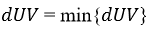
\includegraphics[scale=0.8] {figures/single.PNG}
    \label{fig:my_label}
\end{figure}

Keterangan : 
\par\textit{dUV} : adalah jarak antara data U dan V dari masing-masing cluster U dan V. 
\vspace{5cm}

\subsubsection{\textit{Average  Linkage}} 
\par
\par \textit{Average  Linkage(AVERAGE)} menentukan kedekatan diantara dua kelompok dari jarak rata-rata antar dua data dari cluster yang berbeda. 
Formulasi untuk average linkage adalah : 
\begin{figure} [htbp]
\centering
    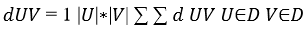
\includegraphics[scale=0.8] {figures/Average.PNG}
    \label{fig:my_label}
\end{figure}

Keterangan : 
\par U dan V adalah jumlah data yang ada dalam cluster U dan V. 
\vspace{1cm}

\subsubsection{\textit{Complete linkage}} 
\par
\textit{Complete linkage(MAX)} menentukan kedekatan diantara dua kelompok dari jarak terjauh (terbesar) antara dua data dari cluster yang berbeda. Formulasi untuk complete linkage adalah : 

\par Formulasi untuk \textit{Single Linkage (MIN)} adalah :
\begin{figure} [htbp]
\centering
    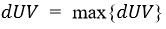
\includegraphics[scale=0.8] {figures/Complete.PNG}
    \label{fig:my_label}
\end{figure}

Keterangan : 
\par\textit{dUV} : adalah jarak antara data U dan V dari masing-masing cluster U 
dan V. 

\subsection{Implementasi \textit{Hierarchical Clustering}}
\subsubsection{implementasi \textit{Hierarchical Clustering} pada Data Musik}

\par\textbf{Extraksi File Musik Dengan Feature Extraction Menggunakan Library Pyaudioanalysis}

\par\hspace{0.5cm}PyAudioAnalysis dapat digunakan untuk mengekstrak fitur audio, melatih dan menerapkan pengklasifikasian audio, mensegmentasikan stream audio dan memvisualisasikan hubungan konten. Library  ini ditulis dengan Python, yang merupakan bahasa pemrograman tingkat tinggi yang telah menarik banyak peminat, terutama dalam komunitas akademis dan ilmiah selama beberapa tahun terakhir.\citep*{giannakopoulos2015pyaudioanalysis}  



Untuk dapat menggunakan fitur ekstraksi pada library  pyAudioAnalysis diharuskan melakukan tahap-tahap berikut ini: 
\begin{enumerate}
    \item Melakukan instalasi python
    \item Melakukan clone pada library  pyAudioAnalysis, sebelum perintah git clone dijalankan, terlebih dahulu masuk kedalam direktori yang diinginkan untuk menyimpanan Library  pyAudioAnalysis,  seperti “cd ujicoba”.
    \item inputkan perintah dibawah pada terminal untuk melakukan clone library   “git clone https://github.com/tyiannak/pyAudioAnalysis.git”.
\end{enumerate}
\begin{figure} [htbp]
    \centering
    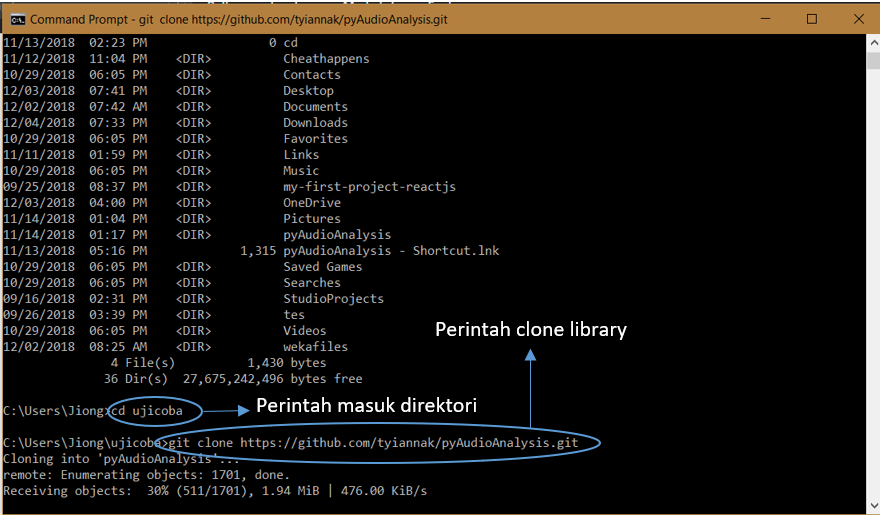
\includegraphics[scale=0.25] {figures/image009.png}
    \caption{\textit{ Clone library}}
\end{figure}
\par\textbf{Install Dependencies Yang Digunakan Oleh Library  pyaudioanalysis }
\begin{enumerate}
    \item  NUMPY  : pip install numpy
    \par\hspace{1cm} Pada terminal terlihat dependencies NUMPY sudah terinstall dan file installan berada pada direktori c:\programdata\anaconda3\lib\sitepackages (1.15.1). Numpy adalah pustaka fundamental untuk perhitungan numerik menggunakan Python. Ini terutama digunakan untuk array,  representasi matriks dan penanganan, beserta dengan satu set fungsi array dasar masing-masing.
    
    \begin{figure} [htbp]
    \centering
    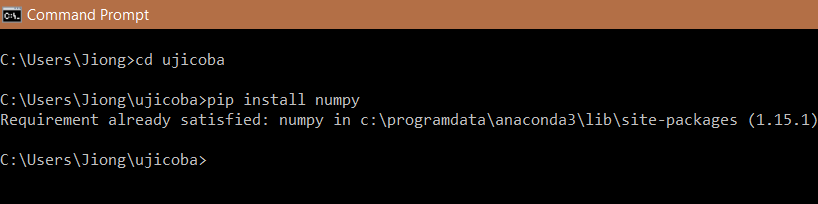
\includegraphics[scale=0.4] {figures/image011.png}
    \caption{\textit{ Install Dependencies NUMPY }}
    \end{figure}
  
    \item MATPLOTLIB  : pip install matplotlib
    \par\hspace{1cm}Pada terminal terlihat dependencies MATPLOTLIB sudah terinstall dan file installan berada pada direktori c:\programdata\anaconda3\lib\sitepackages (2.2.3). Matplotlib menawarkan fungsionalitas penggambaran 2D, mirip dengan MATLAB
    
    \begin{figure} [htbp]
    \centering
    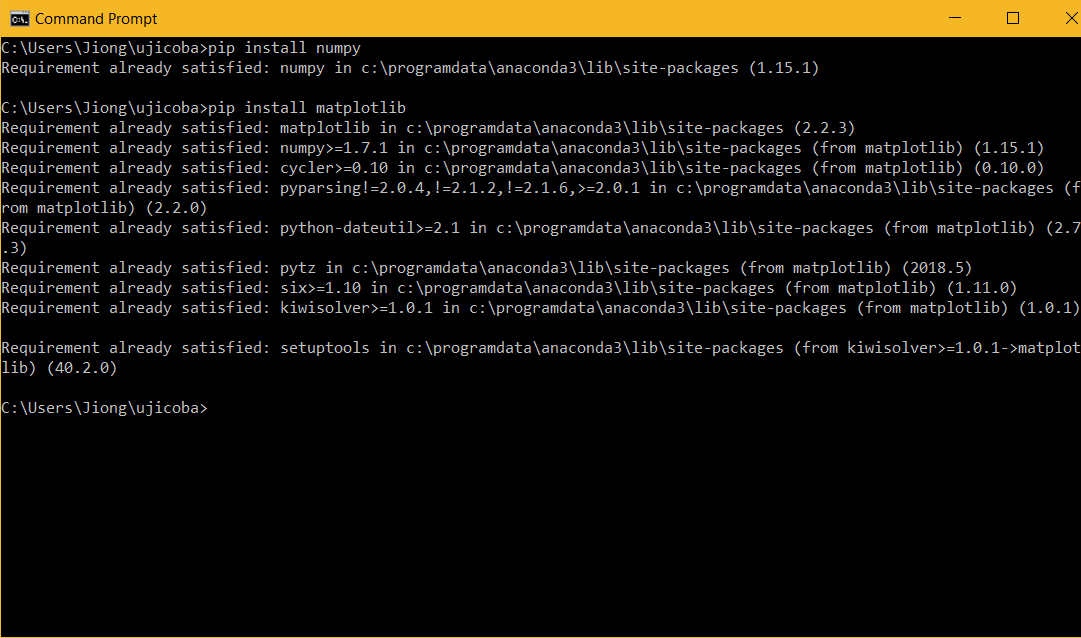
\includegraphics[scale=0.3] {figures/image013.png}
    \caption{\textit{ Install Dependencies MATPLOTLIB  }}
    \end{figure}
  
    
    \item SCIPY  : pip install scipy
    \par\hspace{1cm} Pada terminal terlihat dependencies SCIPY sudah terinstall dan file installan berada pada direktori c:\programdata\anaconda3\lib\sitepackages (1.1.0). SciPy adalah inti dari ekosistem berbasis SciPy Python yang menyediakan komputasi numerik yang dioptimalkan dan rutinitas ilmiah. pyAudioAnalysis menggunakan SciPy untuk prosedur pemrosesan sinyal dasar (misalnya konvolusi), perhitungan linear, perhitungan FFT dan file GELOMBANG IO. 
 
    \begin{figure} [htbp]
    \centering
    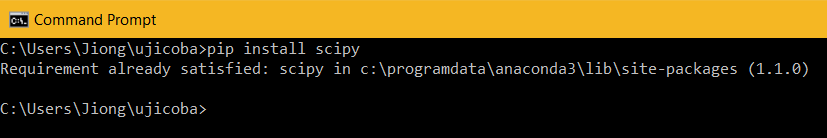
\includegraphics[scale=0.5] {figures/image015.png}
    \caption{\textit{ Install Dependencies SCIPY   }}
    \end{figure}
    
    \item SKLEARN   : pip install sklearn 
    \par\hspace{1cm} Pada terminal terlihat dependencies SKLEARN sudah terinstall dan file installan berada pada direktori c:\programdata\anaconda3\lib\sitepackages (0.0). SKLEARN adalah library  machine learning untuk bahasa pemrograman Python. Library  ini memiliki fitur seperti classification, regression dan algoritma clustering termasuk support vector machines, random forests , gradient boosting , k -means and DBSCAN, dan SKLEARN  dirancang untuk beroperasi dengan library  numerik dan ilmiah Python NumPy dan SciPy. 
 
    \begin{figure} [htbp]
    \centering
    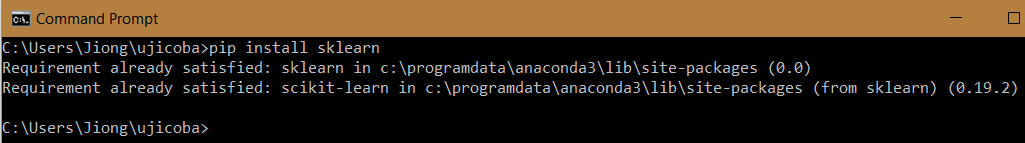
\includegraphics[scale=0.4] {figures/image017.png}
    \caption{\textit{ Install Dependencies SKLEARN   }}
    \end{figure}
    
     
    \item HMMLEARN    : pip install hmmlearn  
    \par\hspace{1cm} Pada terminal terlihat dependencies HMMLEARN sudah terinstall dan file installan berada pada direktori c:\programdata\anaconda3\lib\sitepackages (0.2.1). Library  HMMLEARN adalah algoritma dan model sederhana untuk mempelajari HMM ( Hidden Markov Models ) dengan Python, Dibangun dalam library  scikit-learn, NumPy, SciPy, dan matplotlib. Library  HMMLEARN merupakan library  Open source dan dapat digunakan secara komersial.
 
    \begin{figure} [htbp]
    \centering
    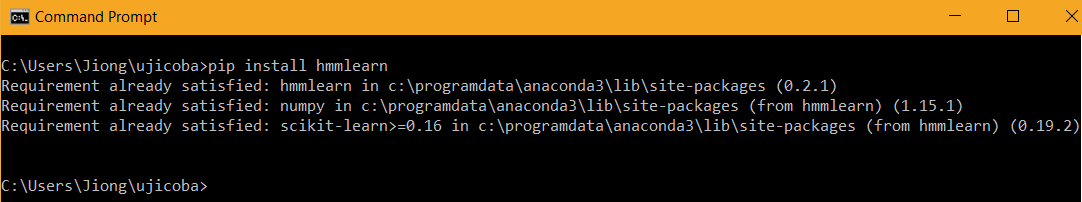
\includegraphics[scale=0.4] {figures/image019.png}
    \caption{\textit{ Install Dependencies hmmlearn    }}
    \end{figure}
   
      
    \item Simplejson     : pip install Simplejson   
    \par\hspace{1cm} Pada terminal terlihat dependencies Simplejson sudah terinstall dan file installan berada pada direktori c:\programdata\anaconda3\lib\sitepackages (3.16.0). Library  Simplejson memaparkan API dari library  marshal dan modul pickle . Ini adalah versi library  json dipelihara secara eksternal yang terdapat dalam Python 2.6, tetapi mempertahankan kompatibilitas dengan Python 2.5 dan memiliki keunggulan kinerja yang signifikan, bahkan tanpa menggunakan ekstensi C opsional untuk percepatan. simplejson juga didukung pada Python 3.3+. 
 
    \begin{figure} [htbp]
    \centering
    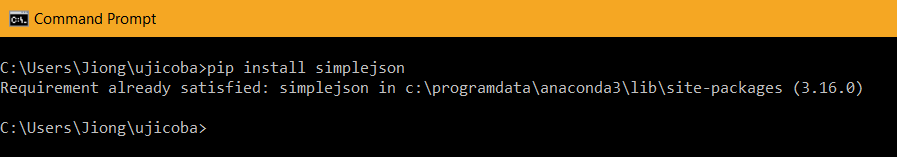
\includegraphics[scale=0.5] {figures/image021.png}
    \caption{\textit{ Install Dependencies Simplejson    }}
    \end{figure}
     

      \item eyeD3      : pip install eyeD3    
    \par\hspace{1cm} Pada terminal terlihat dependencies eyeD3 sudah terinstall dan file installan berada pada direktori c:\programdata\anaconda3\lib\sitepackages (0.8.7). eyeD3 adalah tools dari Python untuk bekerja dengan file audio, khususnya file MP3 yang berisi metadata ID3 (yaitu info lagu), misalnya untuk mengatur beberapa informasi lagu dalam file mp3. Library  ini menyediakan command-line tool (eyeD3) dan library  Python ( import eyed3 ) yang dapat digunakan untuk menulis aplikasi anda sendiri yang dapat dipanggil dari command-line tool. 
 
  
 
    \begin{figure} [htbp]
    \centering
    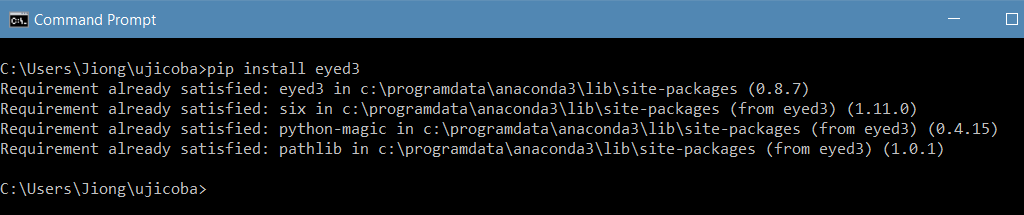
\includegraphics[scale=0.5] {figures/image023.png}
    \caption{\textit{ Install Dependencies eyeD3     }}
    \end{figure}
    
          \item pydub       : pip install pydub     
    \par\hspace{1cm} Pada terminal terlihat dependencies pydub sudah terinstall dan file installan berada pada direktori c:\programdata\anaconda3\lib\sitepackages (0.23.0). 
 \begin{figure} [htbp]
    \centering
    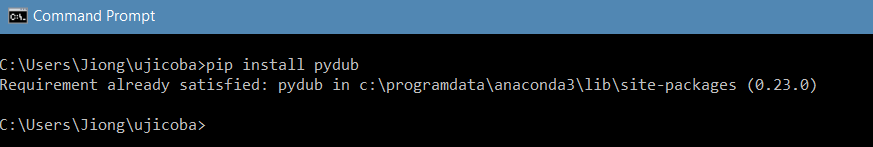
\includegraphics[scale=0.5] {figures/image025.png}
    \caption{\textit{ Install Dependencies pydub}}
    \end{figure}
\end{enumerate}


  \par\textbf{Mengubah Format File Musik Dari Mp3 Mejadi Wav }
    \par\hspace{1cm}Library  sudah dapat digunakan, sebelum menjalankan feature extraction file musik harus di rubah kedalam format WAV, dengan perintah berikut: “python audioAnalysis.py dirMp3toWav -i datamusik/ -r 16000 -c 1” Perintah diatas mengubah data musik yang berada pada direktori datamusik    dari format mp3 menjadi WAV. \begin{figure} [htbp]
    \centering
    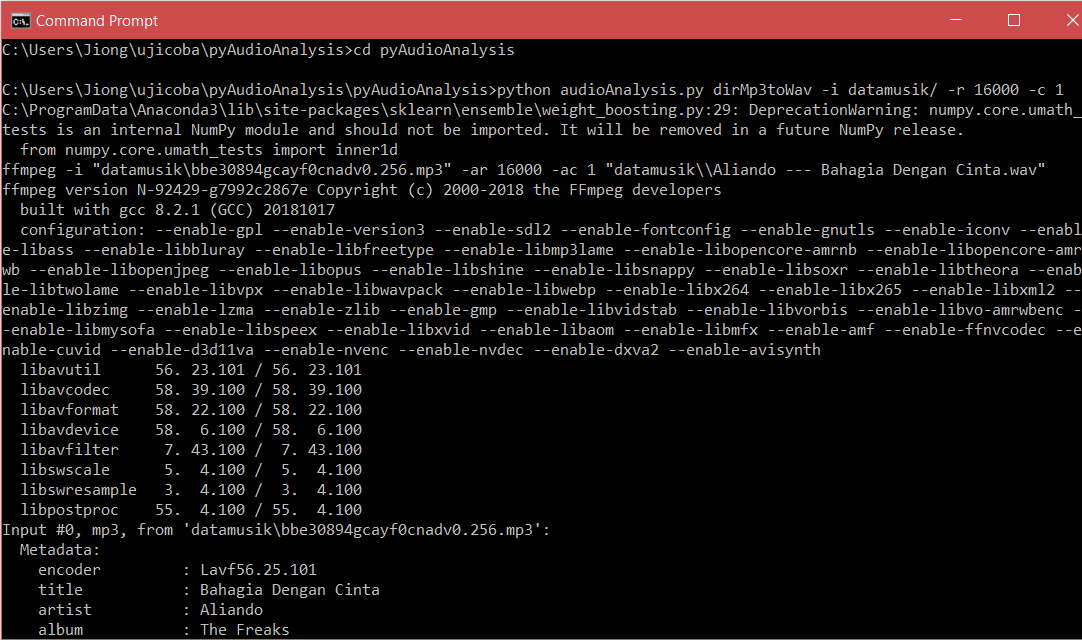
\includegraphics[scale=0.35] {figures/image027.png}
    \caption{\textit{ convert mp3 to WAV}}
    \end{figure}

    \par\hspace{1cm}Pada gambar dibawah terlihat semua file musik pada direktori datamusik sudah diubah menjadi file yang memiliki format .WAV  dari yang awalnya berformat mp3. 
    \begin{figure} [htbp]
    \centering
    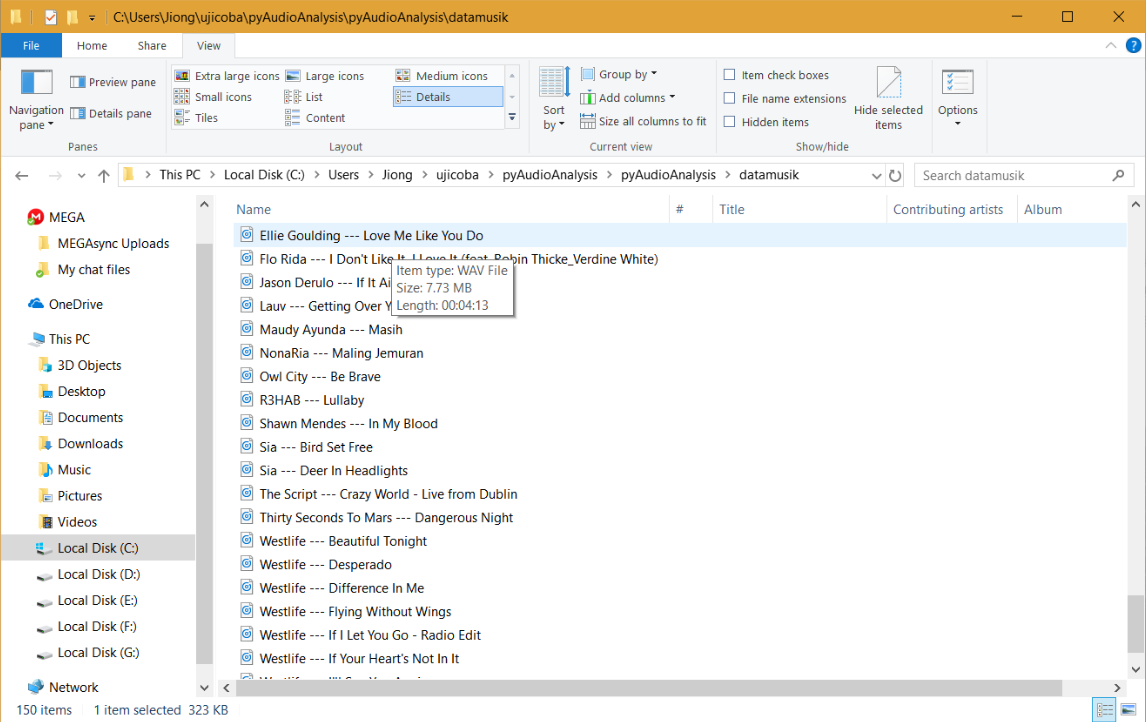
\includegraphics[scale=0.4] {figures/realimage029.PNG}
    \caption{\textit{ Hasil convert mp3 to WAV }}
    \end{figure}

\par\textbf{Menjalankan Ekstraksi Musik Menggunakan Feature Extraction}
    \par\hspace{1cm}Menjalankan fungsi feature extraction pada library  pyAudioAnalysis dengan  perintah : “python audioAnalysis.py  featureExtractionDir -i datamusik / -mw 1.0 -ms 1.0 -sw 0.050 -ss 0.050”.  Perintah ini akan mengekstrak semua file musik yang memiliki format .WAV pada direktori datamusik yang memiliki output CSV.  \begin{figure} [htbp]
    \centering
    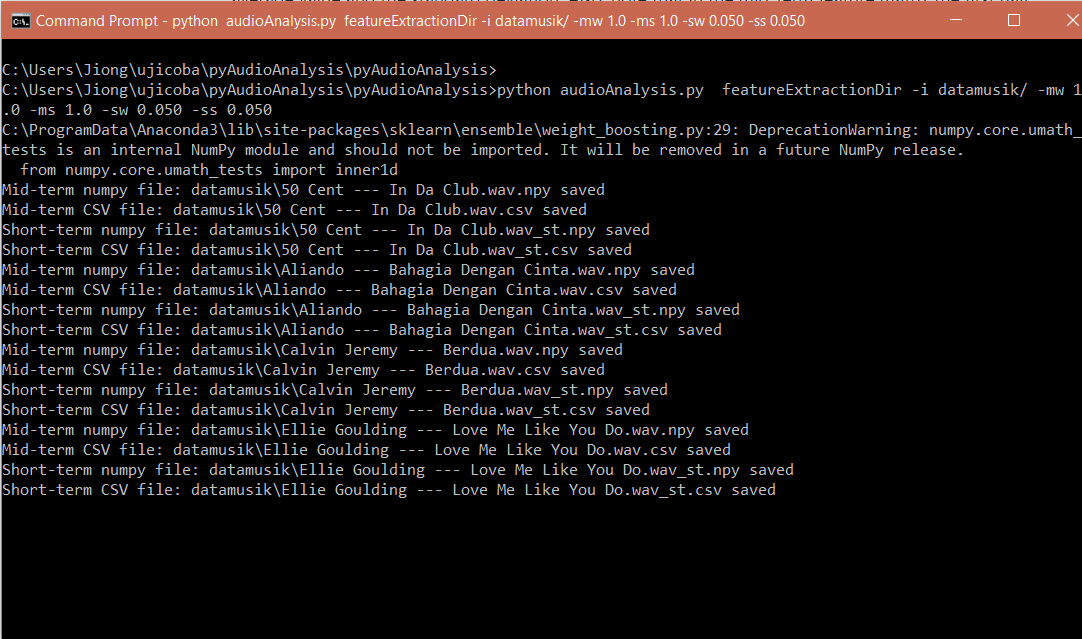
\includegraphics[scale=0.4] {figures/image031.png}
    \caption{\textit{fungsi feature extraction }}
    \end{figure}
    
    Pada gambar dibawah terlihat semua file musik pada direktori data musik yang memiliki format .WAV  sudah diekstraksi dan hasil ekstraksi setiap lagu akan menghasilkan  file csv. Kemudian data tersebut di processing dengan menggabungkan semua data kedalam 1 file csv. 
     \begin{figure} [htbp]
    \centering
    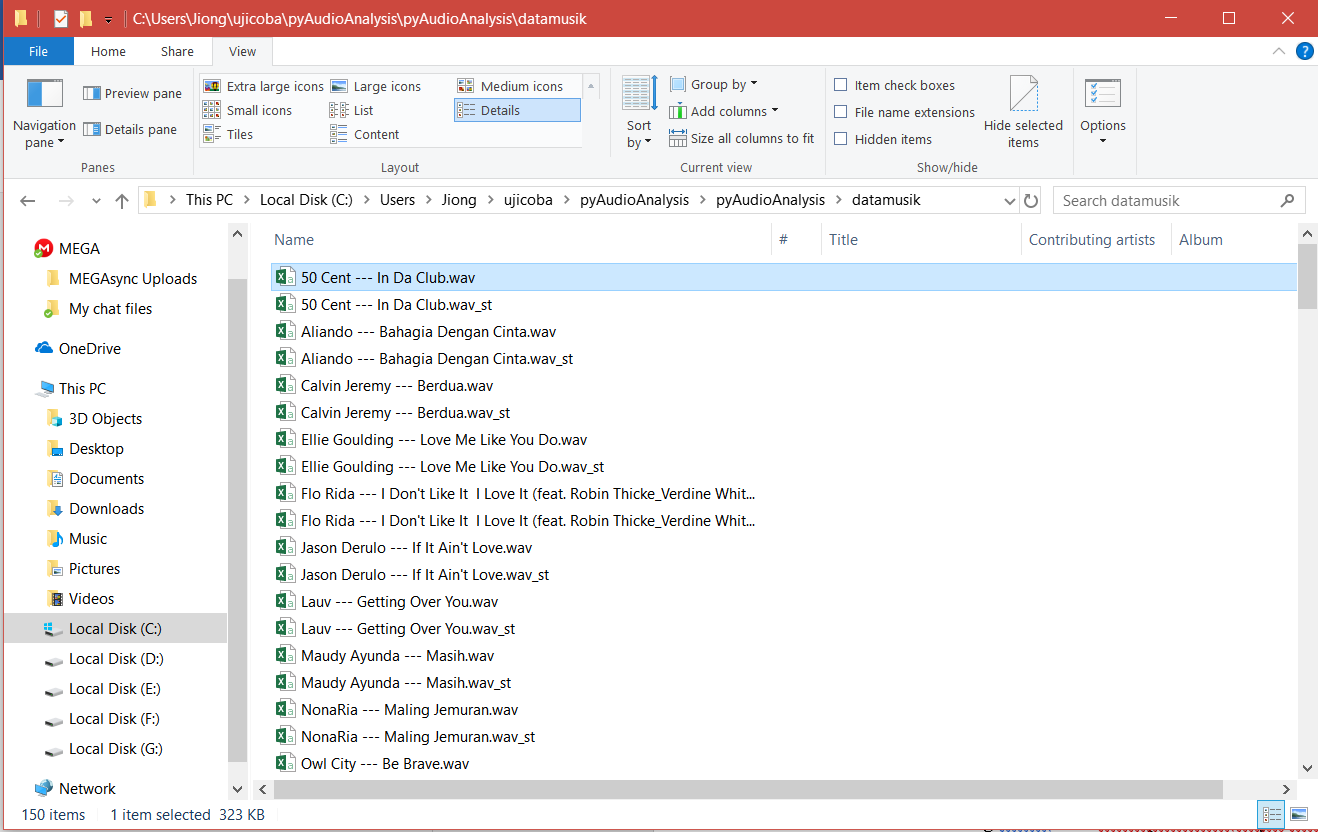
\includegraphics[scale=0.35] {figures/image033.png}
    \caption{\textit{Output fungsi feature extraction}}
    \end{figure}
\par\textbf{Penerapan Algoritma Agglomerative Hierachical Pada Content Musik} 

% Please add the following required packages to your document preamble:
% \usepackage{graphicx}
% \usepackage[normalem]{ulem}
% \useunder{\uline}{\ul}{}
\begin{table}[htbp]
\captionsetup{singlelinecheck=off}
\caption{Nilai atribut tiap musik}
\label{test}
\resizebox{\textwidth}{!}{%
\begin{tabular}{|l|l|l|l|l|l|l|l|l|l|l|l|}
\hline
Judul & \begin{tabular}[c]{@{}l@{}}Zero Crossing \\ Rate\end{tabular} & Energy & \begin{tabular}[c]{@{}l@{}}Entropy \\ of Energy\end{tabular} & \begin{tabular}[c]{@{}l@{}}Spectral \\ Centroid\end{tabular} & \begin{tabular}[c]{@{}l@{}}Spectral \\ Spread\end{tabular} & \begin{tabular}[c]{@{}l@{}}Spectral \\ Entropy\end{tabular} & \begin{tabular}[c]{@{}l@{}}Spectral\\ Flux\end{tabular} & \begin{tabular}[c]{@{}l@{}}Spectral \\ Rolloff\end{tabular} & MFCCs & \begin{tabular}[c]{@{}l@{}}Chroma \\ Vector\end{tabular} & \begin{tabular}[c]{@{}l@{}}Chroma \\ Deviation\end{tabular} \\ \hline
1 & 0.11 & 0.05 & 3.14 & 0.20 & 0.22 & 0.96 & 0.01 & 0.16 & -1.69 & 0.02 & 0.03 \\ \hline
2 & 0.12 & 0.07 & 3.19 & 0.23 & 0.23 & 1.10 & 0.01 & 0.21 & -1.67 & 0.02 & 0.03 \\ \hline
3 & 0.11 & 0.09 & 3.17 & 0.24 & 0.25 & 0.93 & 0.01 & 0.18 & -1.67 & 0.02 & 0.04 \\ \hline
4 & 0.07 & 0.02 & 3.17 & 0.15 & 0.20 & 0.42 & 0.01 & 0.09 & -1.80 & 0.02 & 0.03 \\ \hline
5 & 0.10 & 0.09 & 3.13 & 0.23 & 0.25 & 0.81 & 0.01 & 0.16 & -1.57 & 0.02 & 0.04 \\ \hline
6 & 0.07 & 0.04 & 3.17 & 0.17 & 0.21 & 0.48 & 0.01 & 0.10 & -1.67 & 0.02 & 0.04 \\ \hline
7 & 0.09 & 0.05 & 3.17 & 0.21 & 0.23 & 0.70 & 0.02 & 0.15 & -1.75 & 0.02 & 0.06 \\ \hline
8 & 0.10 & 0.05 & 3.16 & 0.20 & 0.21 & 0.88 & 0.01 & 0.16 & -1.82 & 0.02 & 0.04 \\ \hline
9 & 0.10 & 0.07 & 3.16 & 0.23 & 0.24 & 0.91 & 0.01 & 0.17 & -1.58 & 0.02 & 0.05 \\ \hline
10 & 0.14 & 0.06 & 3.22 & 0.25 & 0.24 & 1.28 & 0.01 & 0.23 & -1.64 & 0.02 & 0.03 \\ \hline
\end{tabular}%
}
\end{table}

% Please add the following required packages to your document preamble:
% \usepackage{graphicx}
\begin{table}[htbp]
\centering
\caption{Penamaan musik}
\label{tab:my-table}
\resizebox{0.8\textwidth}{!}{%
\begin{tabular}{|l|l|}
\hline
\textbf{Inisial} & \textbf{Judul} \\ \hline
1 & Aliando --- Jatuh Cinta Tak Ada Logika \\ \hline
2 & Anne-Marie --- Ciao Adios \\ \hline
3 & bruno mars- just the way you are \\ \hline
4 & Hanin Dhiya --- Darling – Acoustic \\ \hline
5 & Jason Derulo --- Colors \\ \hline
6 & Jason Mraz --- Bella Luna \\ \hline
7 & Jessie J --- I Got You (I Feel Good) \\ \hline
8 & Julia Michaels --- Issues \\ \hline
9 & Calum Scott --- Give Me Something \\ \hline
10 & linkin park- burn it down \\ \hline
\end{tabular}%
}
\end{table}

% Please add the following required packages to your document preamble:
% \usepackage{graphicx}
\begin{table}[htbp]
\centering
\caption{Kriteria Kluster}
\label{tab:my-table}
\resizebox{0.8\textwidth}{!}{%
\begin{tabular}{|l|l|}
\hline
Kluster & Kriteria \\ \hline
K1 & Contenment (menenangkan, relaksasi, damai) \\ \hline
K2 & Exuberance (riuh, bersemangat, bergembira) \\ \hline
K3 & Depression (sedih, murung, depresi, duka) \\ \hline
K4 & Anxious (amarah, kacau, konflik) \\ \hline
\end{tabular}%
}
\end{table}

\vspace{5cm}
\begin{enumerate}
    \item  Dari data ekstraksi musik pada Tabel \ref{test} akan dihitung  matrik jarak antar data menggunakan matrik Euclidian Distance, dengan rumus :
    \begin{figure} [htbp]
    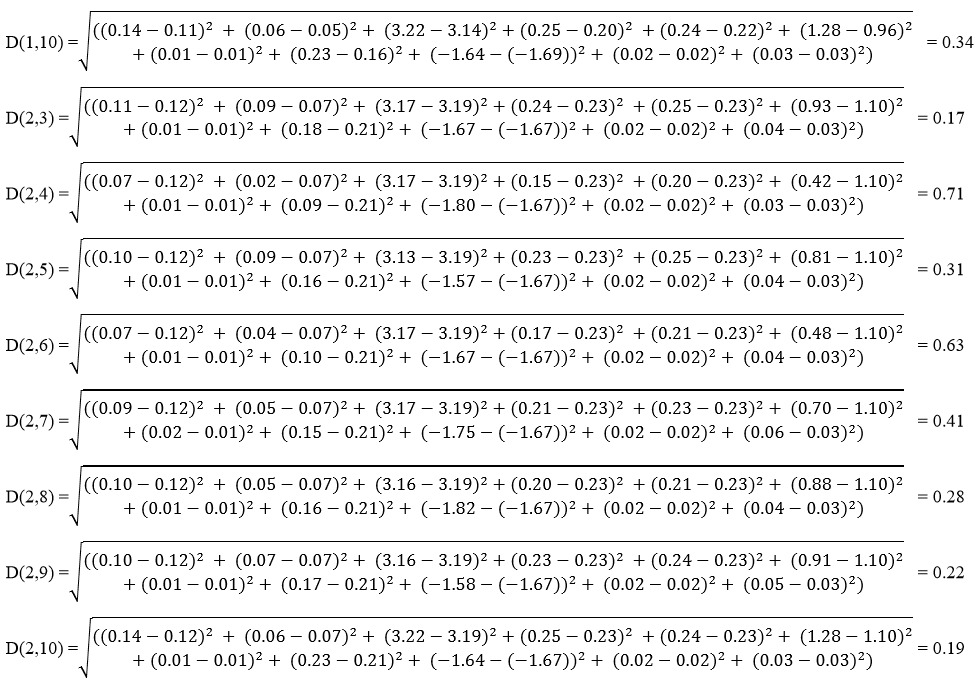
\includegraphics[scale=0.32]{figures/AHC1.jpg}
    \end{figure}
    
    \begin{figure} [htbp]
    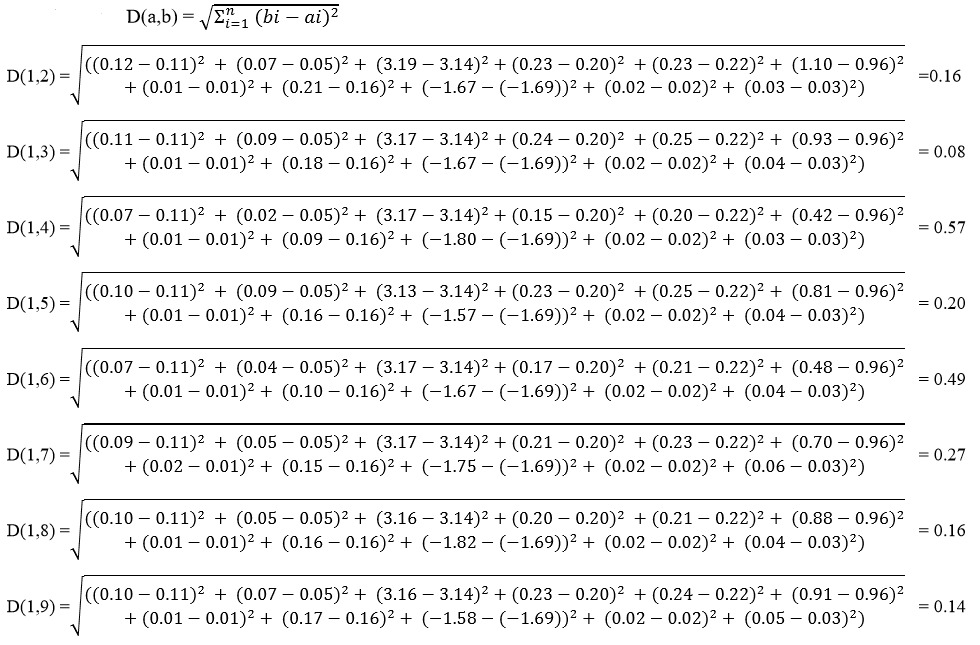
\includegraphics[scale=0.32] {figures/AHC2.jpg}
    \end{figure}
    \vspace{4cm}
    
    \begin{figure} [htbp]
    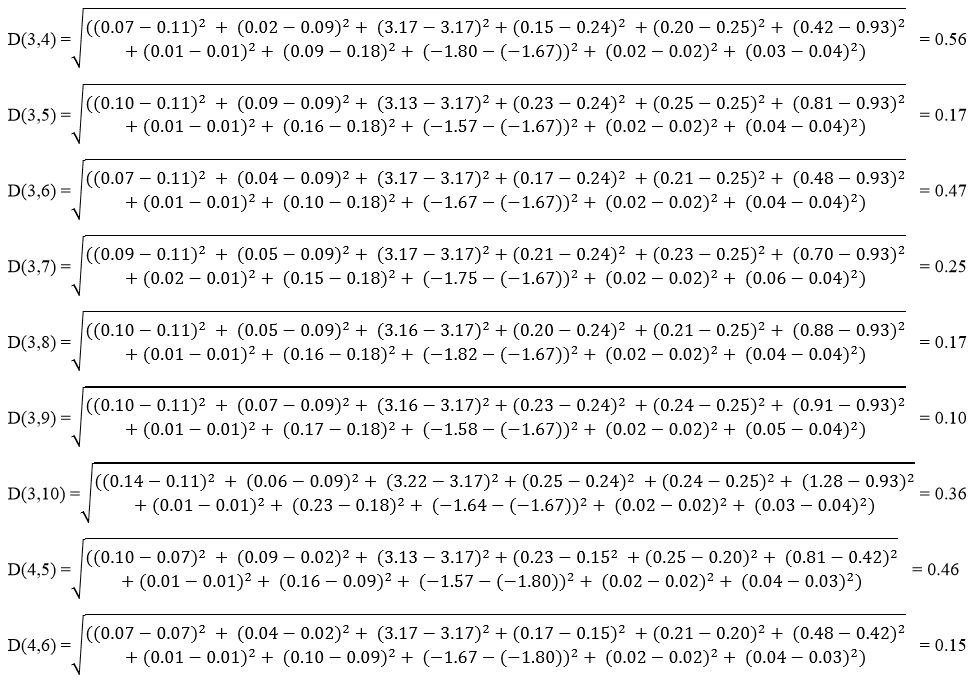
\includegraphics[scale=0.53] {figures/AHC3.PNG}
    \end{figure}
       
    
    \begin{figure} [htbp]
    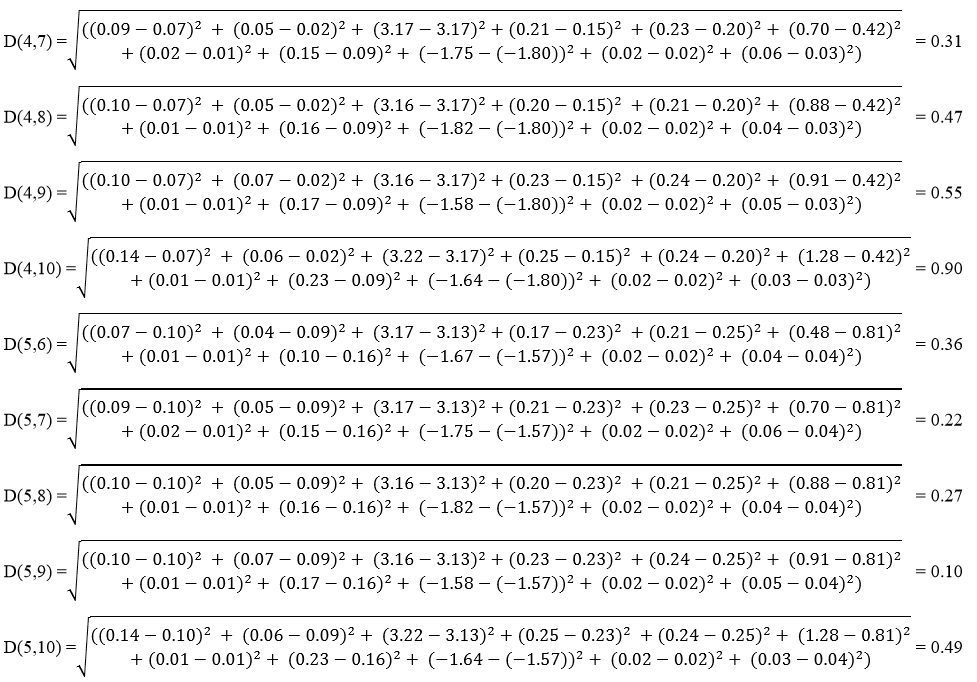
\includegraphics[scale=0.53] {figures/AHC4.PNG}
    \end{figure}
       \vspace{5cm}

    
    \begin{figure} [htbp]
    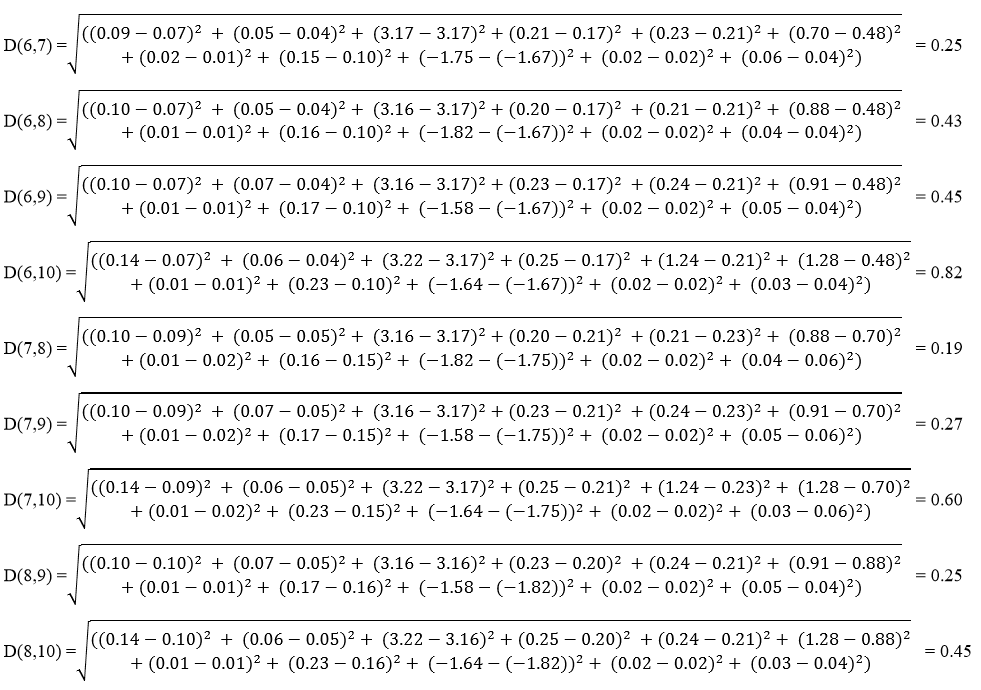
\includegraphics[scale=0.52] {figures/AHC5.PNG}
    \end{figure}
   
    \begin{figure} [htbp]
    \includegraphics[scale=0.7] {figures/66.PNG}
    \end{figure}
       \vspace{6cm}
    
% Please add the following required packages to your document preamble:
% \usepackage{graphicx}
\begin{table}[htbp]
\centering
\caption{Matrik Jarak, dengan Euclidian Distance}
\label{tab:my-table}
\resizebox{0.7\textwidth}{!}{%
\begin{tabular}{|l|l|l|l|l|l|l|l|l|l|l|}
\hline
 & 1 & 2 & 3 & 4 & 5 & 6 & 7 & 8 & 9 & 10 \\ \hline
1 &  & 0.16 & 0.08 & 0.57 & 0.20 & 0.49 & 0.27 & 0.16 & 0.14 & 0.34 \\ \hline
2 & 0.16 &  & 0.17 & 0.71 & 0.31 & 0.63 & 0.41 & 0.28 & 0.22 & 0.19 \\ \hline
3 & 0.08 & 0.17 &  & 0.56 & 0.17 & 0.47 & 0.25 & 0.17 & 0.10 & 0.36 \\ \hline
4 & 0.57 & 0.71 & 0.56 &  & 0.48 & 0.15 & 0.31 & 0.47 & 0.55 & 0.90 \\ \hline
5 & 0.20 & 0.31 & 0.17 & 0.48 &  & 0.36 & 0.22 & 0.27 & 0.10 & 0.49 \\ \hline
6 & 0.49 & 0.63 & 0.47 & 0.15 & 0.36 &  & 0.25 & 0.43 & 0.45 & 0.82 \\ \hline
7 & 0.27 & 0.41 & 0.25 & 0.31 & 0.22 & 0.25 &  & 0.19 & 0.27 & 0.60 \\ \hline
8 & 0.16 & 0.28 & 0.17 & 0.47 & 0.27 & 0.43 & 0.19 &  & 0.25 & 0.45 \\ \hline
9 & 0.14 & 0.22 & 0.10 & 0.55 & 0.10 & 0.45 & 0.27 & 0.25 &  & 0.39 \\ \hline
10 & 0.34 & 0.19 & 0.36 & 0.90 & 0.49 & 0.82 & 0.60 & 0.45 & 0.39 &  \\ \hline
\end{tabular}%
}
\end{table}

\item Dengan metode complete linkage, selanjutnya dipilih dua jarak cluster yang paling terkecil =MIN(B2:K11) = d13 = 0.08
Perhitungan awal cluster (13) tetap digunakan dikarenakan cluster (13) memiliki jarak paling dekat. Maka dipilih cluster 1 dan 3, sehingga cluster 1 dan 3 digabungkan. Selanjutnya, akan dihitung jarak-jarak antara cluster (13) dengan cluster 2,4,5,6,7,8,9 dan 10.

D(13)2 = MAX(0.16, 0.17) = 0.17

D(13)4 = MAX(0.57, 0.56) = 0.57

D(13)5 = MAX(0.20, 0.17) = 0.17

D(13)6 = MAX(0.49, 0.47) = 0.49

D(13)7 = MAX(0.27, 0.25) = 0.57

D(13)8 = MAX(0.16, 0.17) = 0.17

D(13)9 = MAX(0.14, 0.10) = 0.14

D(13)10 = MAX(0.34, 0.36) = 0.36

% Please add the following required packages to your document preamble:
% \usepackage{graphicx}
\begin{table}[htbp]
\centering
\caption{Matrik Jarak, d(1,3)}
\label{tab:my-table}
\resizebox{0.6\textwidth}{!}{%
\begin{tabular}{|l|l|l|l|l|l|l|l|l|l|}
\hline
\textbf{} & \textbf{1,3} & \textbf{2} & \textbf{4} & \textbf{5} & \textbf{6} & \textbf{7} & \textbf{8} & \textbf{9} & \textbf{10} \\ \hline
\textbf{1,3} &  & 0.17 & 0.57 & 0.20 & 0.49 & 0.27 & 0.17 & 0.14 & 0.36 \\ \hline
\textbf{2} &  &  & 0.71 & 0.31 & 0.63 & 0.41 & 0.28 & 0.22 & 0.19 \\ \hline
\textbf{4} &  &  &  & 0.48 & 0.15 & 0.31 & 0.47 & 0.55 & 0.90 \\ \hline
\textbf{5} &  &  &  &  & 0.36 & 0.22 & 0.27 & \textbf{0.10} & 0.49 \\ \hline
\textbf{6} &  &  &  &  &  & 0.25 & 0.43 & 0.45 & 0.82 \\ \hline
\textbf{7} &  &  &  &  &  &  & 0.19 & 0.27 & 0.60 \\ \hline
\textbf{8} &  &  &  &  &  &  &  & 0.25 & 0.45 \\ \hline
\textbf{9} &  &  &  &  &  &  &  &  & 0.39 \\ \hline
\textbf{10} &  &  &  &  &  &  &  &  &  \\ \hline
\end{tabular}%
}
\end{table}

Selanjutnya dipilih kembali jarak dua cluster terkecil. min(\textbf{dUV} \textit{d}(5,9) = 0.10 dan hitung kembali jarak-jarak antara cluster (5,9) dengan cluster yang tersisa 1.3,2,4,6,7,8 dan 10.

D(5,9)13 = MAX(0.20, 0.14, 0.17, 0.10) = 0.20

D(5,9)2  = MAX(0.31, 0.22) = 0.31

D(5,9)4 = MAX(0.48, 0.55) = 0.55

D(5,9)6 = MAX(0.36, 0.45) = 0.45

D(5,9)7 = MAX(0.22, 0.22) = 0.27

D(5,9)8 = MAX(0.27, 0.25) = 0.27

D(5,9)10 = MAX(0.49, 0.36) = 0.49


% Please add the following required packages to your document preamble:
% \usepackage{graphicx}
\begin{table}[htbp]
\centering
\caption{Matrik Jarak, d(5,9)}
\label{tab:my-table}
\resizebox{0.6\textwidth}{!}{%
\begin{tabular}{|l|l|l|l|l|l|l|l|l|}
\hline
\textbf{} & \textbf{1,3} & \textbf{2} & \textbf{4} & \textbf{5,9} & \textbf{6} & \textbf{7} & \textbf{8} & \textbf{10} \\ \hline
\textbf{1,3} &  & 0.17 & 0.57 & 0.20 & 0.49 & 0.27 & 0.17 & 0.36 \\ \hline
\textbf{2} &  &  & 0.71 & 0.31 & 0.63 & 0.41 & 0.28 & 0.19 \\ \hline
\textbf{4} &  &  &  & 0.55 & \textbf{0.15} & 0.31 & 0.47 & 0.90 \\ \hline
\textbf{5,9} &  &  &  &  & 0.45 & 0.27 & 0.27 & 0.49 \\ \hline
\textbf{6} &  &  &  &  &  & 0.25 & 0.43 & 0.82 \\ \hline
\textbf{7} &  &  &  &  &  &  & 0.19 & 0.60 \\ \hline
\textbf{8} &  &  &  &  &  &  &  & 0.45 \\ \hline
\textbf{10} &  &  &  &  &  &  &  &  \\ \hline
\end{tabular}%
}
\end{table}

Selanjutnya dipilih kembali jarak dua cluster terkecil. min\textit{(dUV)}=4,6) = 0.15 dan hitung kembali jarak-jarak antara cluster (4,6)  dengan cluster yang tersisa 1.3,2,5.9,7,8 dan 10.

D(4,6)13=MAX (0.57,0.56,0.49,0.47)=0.57

D(4,6)2=MAX (0.71,0.63)=0.71

D(4,6)5,9=MAX (0.48,0.55,0.36,0.45)=0.55

D(4,6)7=MAX (0.31,0.25)=0.31

D(4,6)8=MAX (0.47,0.43)=0.47

D(4,6)10=MAX (0.90,0.82)=0.90

% Please add the following required packages to your document preamble:
% \usepackage{graphicx}
\begin{table}[htbp]
\centering
\caption{Matrik Jarak, d(4,6)}
\label{tab:my-table}
\resizebox{0.6\textwidth}{!}{%
\begin{tabular}{|l|l|l|l|l|l|l|l|}
\hline
\textbf{} & \textbf{1,3} & \textbf{2} & \textbf{4,6} & \textbf{5,9} & \textbf{7} & \textbf{8} & \textbf{10} \\ \hline
\textbf{1,3} &  & \textbf{0.17} & 0.57 & 0.20 & 0.27 & 0.17 & 0.36 \\ \hline
\textbf{2} &  &  & 0.71 & 0.31 & 0.41 & 0.28 & 0.19 \\ \hline
\textbf{4,6} &  &  &  & 0.55 & 0.31 & 0.47 & 0.90 \\ \hline
\textbf{5,9} &  &  &  &  & 0.27 & 0.27 & 0.49 \\ \hline
\textbf{7} &  &  &  &  &  & 0.19 & 0.60 \\ \hline
\textbf{8} &  &  &  &  &  &  & 0.45 \\ \hline
\textbf{10} &  &  &  &  &  &  &  \\ \hline
\end{tabular}%
}
\end{table}

Selanjutnya dipilih kembali jarak dua cluster terkecil. min\textit{(dUV)}= d(1,3,2) = 0.17 dan hitung kembali jarak-jarak antara cluster (1,3,2)  dengan cluster yang tersisa 4.6,5.9,7,8 dan 10.

D(1,3,2)4,6 = MAX(0.57,0.56,0.71,0.49,0.47,0.43)=0.71

D(1,3,2)5,9 = MAX(0.20,0.17,0.31,0.14,0.10,0.22)=0.31

D(1,3,2)7 = MAX(0.27,0.25,0.41)=0.41

D(1,3,2)8 = MAX(0.16,0.17,0.28)=0.28

D(1,3,2)10 = MAX(0.34,0.36,0.19)=0.36

% Please add the following required packages to your document preamble:
% \usepackage{graphicx}
\begin{table}[htbp]
\centering
\caption{ Matrik Jarak, d(1,3,2}
\label{tab:my-table}
\resizebox{0.4\textwidth}{!}{%
\begin{tabular}{|l|l|l|l|l|l|l|}
\hline
\textbf{} & \textbf{1,3,2} & \textbf{4,6} & \textbf{5,9} & \textbf{7} & \textbf{8} & \textbf{10} \\ \hline
\textbf{1,3,2} &  & 0.71 & 0.31 & 0.41 & 0.28 & 0.36 \\ \hline
\textbf{4,6} &  &  & 0.55 & 0.31 & 0.27 & 0.90 \\ \hline
\textbf{5,9} &  &  &  & 0.27 & 0.27 & 0.49 \\ \hline
\textbf{7} &  &  &  &  & \textbf{0.19} & 0.60 \\ \hline
\textbf{8} &  &  &  &  &  & 0.45 \\ \hline
\textbf{10} &  &  &  &  &  &  \\ \hline
\end{tabular}%
}
\end{table}

Selanjutnya dipilih kembali jarak dua cluster terkecil. min\textit{(dUV)} \textit{d}(7,8) = 0.19 dan hitung kembali jarak-jarak antara cluster (7,8)  dengan cluster yang tersisa 1.3.2,4.6,5.9, dan 10. 

D(7,8)1,3,2 = MAX(0.27,0.25,0.41,0.16,0.17,0.28)=0.41 
 
D(7,8)4,6 = MAX(0.31,0.25,0.47,0.43)=0.47 

D(7,8)5,9 = MAX(0.22,0.27,0.27,0.25)=0.27 

D(7,8)10 = MAX(0.60,0.45)=0.60 
 
% Please add the following required packages to your document preamble:
% \usepackage{graphicx}
\begin{table}[htbp]
\centering
\caption{ Matrik Jarak, d(7,8) }
\label{tab:my-table}
\resizebox{0.4\textwidth}{!}{%
\begin{tabular}{|l|l|l|l|l|l|}
\hline
\textbf{} & \textbf{1,3,2} & \textbf{4,6} & \textbf{5,9} & \textbf{7,8} & \textbf{10} \\ \hline
\textbf{1,3,2} &  & 0.71 & 0.31 & 0.41 & 0.36 \\ \hline
\textbf{4,6} &  &  & 0.55 & 0.47 & 0.90 \\ \hline
\textbf{5,9} &  &  &  & \textbf{0.27} & 0.49 \\ \hline
\textbf{7,8} &  &  &  &  & 0.60 \\ \hline
\textbf{10} &  &  &  &  &  \\ \hline
\end{tabular}%
}
\end{table}

Selanjutnya dipilih kembali jarak dua cluster terkecil. min\textit{(dUV)} \textit{d}(5,9,7,8) = 0.27 dan hitung kembali jarak-jarak antara cluster (5,9,7,8)  dengan cluster yang tersisa 1.3.2,4.6 dan 10.

D(5,9,7,8)1,3,2 = MAX(0.20,0.17,0.31,0.14,0.10,0.22,0.27,0.25,0.41,0.16,0.17,\\0.28)=0.41

D(5,9,7,8)4,6 = MAX(0.48,0.36,0.55,0.45,0.31.0.25,0.47,0.43)=0.55

D(5,9,7,8)10 = MAX(0.49,0.39,0.60,0.45)=0.60

% Please add the following required packages to your document preamble:
% \usepackage{graphicx}
\begin{table}[htbp]
\centering
\caption{Matrik Jarak, d(5,9,7,8)}
\label{tab:my-table}
\resizebox{0.4\textwidth}{!}{%
\begin{tabular}{|l|l|l|l|l|}
\hline
\textbf{} & \textbf{1,3,2} & \textbf{4,6} & \textbf{5,9,7,8} & \textbf{10} \\ \hline
\textbf{1,3,2} &  & 0.71 & 0.41 & 0.36 \\ \hline
\textbf{4,6} &  &  & 0.55 & 0.90 \\ \hline
\textbf{5,9,7,8} &  &  &  & 0.60 \\ \hline
\textbf{10} &  &  &  &  \\ \hline
\end{tabular}%
}
\end{table}
\end{enumerate}

Hasil akhir dari perhitungan keseluruhan matriks sudah menghasilkan 4 kluster sesuai yang ditentukan sejak awal.

Kluster 1 : (1) Aliando --- Jatuh Cinta Tak Ada Logika, (3) bruno mars- just the             way you are, (2) Anne-Marie --- Ciao Adios

Kluster 2 : (4)Hanin Dhiya --- Darling - Acoustic, (6) Jason Mraz --- Bella Luna

Kluster 3 : (5) Jason Derulo --- Colors, (9) Calum Scott --- Give Me Something,              (7) Jessie J --- I Got You (I Feel Good), (8) Julia Michaels --- Issues

Kluster 4 : (10) linkin park- burn it down

\subsection{ Validasi Hasil Perhitungan Agglomerative Hierarchical Clustering menngunakan tools RapidMiner}
 \begin{figure} [htbp]
    \includegraphics[scale=0.28] {figures/7.PNG}
    \end{figure}
    \vspace{5cm}

\subsection{Soal Latihan}
\begin{enumerate}
    \item Ekstraklah 25 data musik menggunakan library python Pyaudioanalysis lalu implementasikan Metode \textit{Agglomerative Hierarchical clustering} dengan menggunakan teknik pendekatan : \textit{single linkage}, \textit{complete linkage} dan \textit{ average linkage}, banyak kluster berdasarkan 4 kriteria kluster pada contoh soal dan berikan alasan untuk setiap kluster mengapa musik tersebut tergabung pada kluster itu.
    \item Pada tabel dibawah terdapat data ukuran badan mahasiswa, kelompokanlah data tersebut menjadi 2 kelompok dengan menggunakan teknik pendekatan : \textit{single linkage}, \textit{complete linkage} dan \textit{ average linkage}. 
    % Please add the following required packages to your document preamble:
% \usepackage{graphicx}
\begin{table}[htbp]

\label{tab:my-table}
\resizebox{\textwidth}{!}{%
\begin{tabular}{|c|c|c|c|c|c|}
\hline
\multicolumn{1}{|l|}{\textbf{Nama}} & \multicolumn{1}{l|}{\textbf{Tinggi(cm)}} & \multicolumn{1}{l|}{\textbf{Berat(kg)}} & \multicolumn{1}{l|}{\textbf{\begin{tabular}[c]{@{}l@{}}Lingkar  \\ Tangan(cm)\end{tabular}}} & \multicolumn{1}{l|}{\textbf{\begin{tabular}[c]{@{}l@{}}Lingkar \\ Pinggang(cm)\end{tabular}}} & \multicolumn{1}{l|}{\textbf{\begin{tabular}[c]{@{}l@{}}Lingkar \\ Paha(cm)\end{tabular}}} \\ \hline
Brandon & 180 & 88 & 40 & 64 & 75 \\ \hline
Kent & 155 & 68 & 50 & 68 & 67 \\ \hline
Jess & 189 & 77 & 55 & 69 & 51 \\ \hline
Zxuan & 200 & 79 & 45 & 84 & 59 \\ \hline
Bruno & 178 & 65 & 35 & 70 & 88 \\ \hline
Lesley & 188 & 59 & 34 & 75 & 77 \\ \hline
Granger & 198 & 57 & 24 & 88 & 66 \\ \hline
Fanny & 145 & 68 & 28 & 94 & 51 \\ \hline
Lancelot & 154 & 99 & 51 & 58 & 48 \\ \hline
Rias Gremory & 165 & 91 & 26 & 64 & 77 \\ \hline
\end{tabular}%
 }
\end{table}
\end{enumerate}


\chapter{TEXT MINING}
\section{Teknik Preprocessing}
    \subsection{Porter Algoritma}
        Stemmer yang paling sering digunakan adalah Algoritma Porter. 
        Porter Stemmer akan menghilangkan afiks dari suatu kata dengan ingkat berdasarkan semua aturan dan kondisi dari kata tersebut. 
        Karena tidak mempertimbangkan kosa kata dan arti dari kata itu sendiri maka algoritma porter sering dikira \textit{error}. 
        Kata-kata yang memiliki arti yang berbeda direduksi menjadi stem yang sama, misalnya ``\textit{generic}`` dan ``\textit{generation}`` akan di stem menjadi ``\textit{gener}``. 
        Sementara kata-kata yang memiliki makna serupa tidak dapat direduksi menjadi stem umum sama sekali, misalnya ``\textit{recognition}`` dan ``\textit{recognize}``. 
        Selain itu hasil stem yang dihasilkan mungkin bukan kata yang valid, tetapi Algoritma Porter Stemmer tetap menunjukkan hasil yang baik dan salah satu yang terbaik dalam Information Retrieval.
        \par Porter stemmer dikembangkan oleh Martin Porter pada tahun 1980 di University of Cambridge. 
        Algoritma Porter diterapkan pada langkah pre-processing untuk text mining, fungsi utamanya adalah sebagai bagian dari proses normalisasi istilah yang biasanya dilakukan ketika membuat sistem pencarian informasi. 
        \par Selain itu algoritma stemmer ini juga digunakan pada bidang lainnya seperti klasifikasi teks, klustering teks, dan \textit{spam filtering}. 
        \par Algoritma Porter Stemmer didasarkan pada gagasan bahwa akhiran atau sufiks dalam bahasa inggris sebagian besar terdiri dari kombinasi dari sufiks yang lebih kecil dan lebih sederhana. 
        Kelemahan algoritma porter adalah hasil stemming tidak selalu menghasilkan \textit{real words}.
        Terdapat 6 langkah Stemming pada Algoritma Porter dan dalam setiap langkah memiliki aturan tersendiri. Berikut pada gambar \ref{6step} adalah penjelasannya:
       
        \begin{figure}
            \centerline {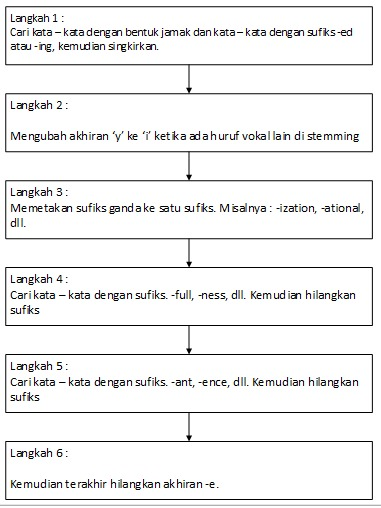
\includegraphics[width=0.65\textwidth]
            {chapters/figures/porter_step.PNG}}
            \caption{Langkah-langkah \textit{Algoritma Porter}}
            \label{6step}
        \end{figure}

\begin{enumerate}
    \item Langkah 1 : hilankan sufiks –ed dan –ing.
    \vspace{3 cm}
\begin{table}[]
\centering
\begin{tabular}{|l|l|l|}
\hline
Kata-kata & Peraturan  & Hasil \\ \hline
\begin{tabular}[c]{@{}l@{}}amaze, amazed,\\ amazedly, amazedness\end{tabular} & \begin{tabular}[c]{@{}l@{}}-ly dan -ed\\ -ss dan -ed\end{tabular}   & amaz, amaz, amaz, amaz \\ \hline
\begin{tabular}[c]{@{}l@{}}amazing, amazingly, \\ amazingness\end{tabular}    & \begin{tabular}[c]{@{}l@{}}-ly dan -ing\\ -ss dan -ing\end{tabular} & amaz, amaz, amaz       \\ \hline
\end{tabular}
\end{table}

    \item Langkah 2 : mengubah sufiks `y` ke `i`.
    \vspace{3 cm}
\begin{table}[]
\centering
\begin{tabular}{|l|l|l|}
\hline
Kata-kata & Peraturan & Hasil \\ \hline
cry       & -y ke -i  & cri   \\ \hline
dry       & -y ke -i  & dri   \\ \hline
\end{tabular}
\end{table}

    \item Langkah 3 : Memetakan sufiks ganda ke sufiks \textit{single}.
    % \vspace{3 cm}
\begin{table}[]
\centering
\begin{tabular}{|l|l|l|}
\hline
Kata-kata & Peraturan          & Hasil  \\ \hline
national  & -ational ke -ation & nation \\ \hline
\end{tabular}
\end{table}

    \item Langkah 4 : hilangkan sufiks -ness dan -full.
    % \vspace{3 cm}
\begin{table}[]
\centering
\begin{tabular}{|l|l|l|}
\hline
Kata-kata & Peraturan          & Hasil  \\ \hline
kindess  & -ness - & kind \\ \hline
\end{tabular}
\end{table}

    \item Langkah 5 : hilangkan sufiks -ant, -ance dan -ence.
\begin{table}[]
\centering
\begin{tabular}{|l|l|l|}
\hline
Kata-kata & Peraturan          & Hasil  \\ \hline
compliance  & -ance - & compli \\ \hline
\end{tabular}
\end{table}

    \item Langkah 6 : hilangkan sufiks -e.
\begin{table}[]
\centering
\begin{tabular}{|l|l|l|}
\hline
Kata-kata & Peraturan          & Hasil  \\ \hline
engine  & -e - & engin \\ \hline
\end{tabular}
\end{table}

\end{enumerate}


\section{Metode \textit{Naïve Bayes Classifier}}
\textit{Naïve Bayes Classifier} merupakan sebuah metoda klasifikasi yang berakar pada teorema Bayes. Metode pengklasifikasian dengan menggunakan metode probabilitas dan statistik yang dikemukakan oleh ilmuwan Inggris Thomas Bayes, yaitu memprediksi peluang di masa depan berdasarkan pengalaman di masa sebelumnya sehingga dikenal sebagai Teorema Bayes. Ciri utama dari \textit{Naïve Bayes Classifier} ini adalah asumsi yang sangat kuat akan independens dari masing-masing kondisi atau kejadian.
\par Menurut Olson dan Delen menjelaskan \textit{Naïve Bayes} untuk setiap kelas keputusan, menghitung probabilitas dengan syarat bahwa kelas keputusan adalah benar, mengingat vektor informasi obyek. Algoritma ini mengasumsikan bahwa atribut obyek adalah independen. Probabilitas yang terlibat dalam memproduksi perkiraan akhir dihitung sebagai jumlah frekuensi dari "\textit{master}" tabel keputusan.
\par Keuntungan penggunan adalah bahwa metoda ini hanya membutuhkan jumlah data pelatihan (\textit{training data}) yang kecil untuk menentukan estimasi parameter yang diperlukan dalam proses pengklasifikasian. Karena yang diasumsikan sebagai variable \textit{independent}, maka hanya varians dari suatu variable dalam sebuah kelas yang dibutuhkan untuk menentukan klasifikasi, bukan keseluruhan dari matriks kovarians.


\par \textbf{Kekurangan Metode \textit{Naïve Bayes Classifier}:}
\begin{enumerate}
    \item 	Tidak berlaku jika probabilitas kondisionalnya adalah nol, apabila nol maka probabilitas prediksi akan bernilai nol juga.
	\item Mengasumsikan variabel bebas.
\end{enumerate}

\par \textbf{Kelebihan Metode \textit{Naïve Bayes Classifier}:}
\begin{enumerate}
    \item Menangani kuantitatif dan data diskrit
    \item Kokoh untuk titik noise yang diisolasi, misalkan titik yang dirata – ratakan ketika mengestimasi peluang bersyarat data.
    \item Hanya memerlukan sejumlah kecil data pelatihan untuk mengestimasi parameter (rata-rata dan variansi dari variabel) yang dibutuhkan untuk klasifikasi.
    \item Menangani nilai yang hilang dengan mengabaikan instansi selama perhitungan estimasi peluang.
    \item Cepat dan efisiensi ruang.
	\item Kokoh terhadap atribut yang tidak relevan.
\end{enumerate}

\par \textbf{Naive Bayes} merupakan sebuah pengklasifikasian probabilistik sederhana yang menghitung sekumpulan probabilitas dengan menjumlahkan frekuensi dan kombinasi nilai dari dataset yang diberikan. Suatu metode yang dapat memprediksi probabilitas keanggotaan kelas suatu data yang akan masuk ke dalam kelas atau kategori tertentu, sesuai dengan perhitungan probabilitas.
\par \textbf{Naïve bayes} dapat digunakan untuk berbagai macam keperluan antara lain untuk klasifikasi dokumen, deteksi spam atau filtering spam, dan masalah klasifikasi lainnya. Pada penelitian ini terdapat Data Latih atau \textbf{Training} dan Data Uji atau \textbf{Testing}.\textbf{ Data Training} menggunakan data yang sebelumnya sudah diinputkan ke dalam aplikasi CMS, kemudian dicari seberapa sering sebuah kata masuk kedalam suatu kategori. Data Uji atau \textbf{Data Testing} adalah data yang akan diuji dan menggunakan perhitungan, kemudian dicari nilai probabilitasnya menggunakan teorema bayes. Teorema bayes merupakan dasar aturan dari \textbf{naive bayes classifier} berikut teorema bayes akan disajikan rumus berikut \ref{nbr}:
\begin{equation}
\label{nbr}
    P(W_n|V_n) = \frac{(n_k + 1)}{(jumlah frekuensi + jumlah kata)} 
\end{equation} 
\par Keterangan \ref{nbr}:
\par P(W_k|V_j) adalah Probabilitas bobot setiap kategori
\par n_k adalah Nilai kemunculan frekuensi kata
\par jumlah frekuensi adalah Jumlah Kemunculan kata pada setiap kategori
\par jumlah kata adalah Jumlah keseluruhan kata pada 

\par Berdasarkan rumus \ref{nbr} akan didapatkan probabilitas setiap kategori yang kemudian akan hitung probabilitas kategori dengan menggunakan rumus sebagai berikut pada \ref{nbb}

\begin{equation}
\label{nbb}
    P(V_j) = \frac{a}{b} 
\end{equation} 

\par Keterangan \ref{nbb}:
\par P(V_j) adalah Probabilitas Kata
\par a adalah Jumlah dokumen pada setiap kategori
\par b adalah Jumlah total keseluruhan dokumen pada data training

\par Setelah itu, setiap kata pada judul dokumen akan dihitung dan dijumlahkan kemudian dihitung probabilitasnya. Kemudian dicari probabilitas mana yang paling besar, maka judul tersebut akan otomatis ke kategori yang memiliki nilai probabilitas tertinggi

\subsection{Contoh Kasus}
Perhitungan dengan menggunakan metode Naïve Bayes Classifier ada proses perhitungan mencari nilai probabilitas yang paling tinggi. Proses ini adalah menghitung setiap kata berdasarkan jumlah kata yang sering muncul pada sebuah kategori. Semakin sering sebuah kata di dalam judul maka nilai probabilitas terhadap kategori tersebut akan semakin tinggi. Penelitian ini menggunakan sebanyak 183 judul dokumen dibagi menjadi 9 kategori. Judul–judul dokumen tersebut didapatkan dari aplikasi CMS sebelumnya dan dijadikan sebagai data training untuk penelitian ini. Berikut 9 kategori judul dokumen:
    \begin{enumerate}
        \item 	Certification Management: Mengolah dokumen tentang sertifikasi dan izin terbang
    	\item Flight Test : Mengolah dokumen hasil tes terbang suatu pesawat.
	    \item Performance & Stability : Mengolah dokumen performa stabilnya mesin pesawat.
	    \item Structure : Mengolah dokumen struktur mesin, cara kerja bagian sebuah pesawat.
        \item Mechanical & Hydrouling : mengolah dokumen hydraulic.
    	\ITEM Electrical System : Mengolah dokumen tentang elektrik dan kelistrikan pesawat.
	    \item Avionic System : Mengolah dokumen test fungsi bagian pesawat.
	    \item Propulsion & Fuel System : Mengolah dokumen bahan bakar.
	    \item Interior and Cabin Safety : Mengolah dokumen design interior cabin suatu pesawat
    \end{enumerate}
    Berikut pada tabel \ref{tab:a} adalah kata kunci dari setiap kategori yang melewati tahap data training:
    \vspace{5 cm}
    \begin{table}[]
    \caption{Tabel Kategori Kata Kunci}
    \label{tab:a}
    \centering
\begin{tabular}{|l|l|}
\hline
Kategori                  & Kata Kunci                                                                                                  \\ \hline
Certification Management  & \begin{tabular}[c]{@{}l@{}}Plan,\\   Certification, Modification, List, Configuration\end{tabular}          \\ \hline
Flight Test               & \begin{tabular}[c]{@{}l@{}}Flight,\\   Test, Certification, Result\end{tabular}                             \\ \hline
Performance \& Stability  & \begin{tabular}[c]{@{}l@{}}Engineering,\\   Justification, Performance, Qualities\end{tabular}              \\ \hline
Structure                 & \begin{tabular}[c]{@{}l@{}}Analysis,\\   Stress, Strenght, Load\end{tabular}                                \\ \hline
Mechanical \& Hydrouling  & \begin{tabular}[c]{@{}l@{}}Hydraulic,\\   Power, Technical\end{tabular}                                     \\ \hline
Electrical System         & \begin{tabular}[c]{@{}l@{}}Electrical,\\   Lighting, Subsystem\end{tabular}                                 \\ \hline
Avionic System            & \begin{tabular}[c]{@{}l@{}}Test,\\   Ground, Result, Procedure, Communication, Record, Require\end{tabular} \\ \hline
Propulsion \& Fuel System & \begin{tabular}[c]{@{}l@{}}Fuel,\\   Hazard, Functional\end{tabular}                                        \\ \hline
Interior and Cabin Safety & \begin{tabular}[c]{@{}l@{}}Interior,\\   Design, Cooling, Cabin, Air Conditioner\end{tabular}               \\ \hline
\end{tabular}
\end{table}

\par Kemudian setelah data training di dapatkan, maka selanjutnya adalah langkah pengujian. Dalam langkah pengujian ini maka akan dijumlahkan nilai probabilitas setiap kata pada setiap kategori kemudian dikalikan dengan probabilitas dokumen yang sudah dihitung. Untuk pengujian, akan dihitung dengan judul dokumen baru yang belum diketahui kategorinya. Judul dokumennya adalah : CN235-220M NAU5 List Of Procedure Certification Plan. Maka langkah pertama adalah melalui proses text mining yaitu preprocessing, kata kata yang di dapat adalah sebagai berikut.
\begin{table}[]
\caption{Tabel Frekuensi Kemunculan Kata}
\begin{tabular}{|l|l|}
\hline
Kata     & Frekuensi \\ \hline
List     & 1         \\ \hline
Proced   & 1         \\ \hline
Certific & 1         \\ \hline
Plan     & 1         \\ \hline
\end{tabular}
\end{table}

\par Pada tabel 1 di dapat banyak frekuensi kemunculan kata pada judul dokumen baru atau data uji, kemudian akan dihitung nilai probabilitasnya pada setiap kategorinya. 
\begin{enumerate}
    \item Kategori 1 – Management
    \begin{table}[]
\begin{tabular}{llll}
\multicolumn{2}{l}{\begin{tabular}[c]{@{}l@{}}P(list |\\ Management)\end{tabular}}     & \multicolumn{2}{l}{= (0+1) : (71) = 0.0141}                                                                         \\
\multicolumn{2}{l}{P(proced | Management)}                                             & \multicolumn{2}{l}{= (0+1) : (71) = 0.0141}                                                                         \\
\multicolumn{2}{l}{\begin{tabular}[c]{@{}l@{}}P(certific |\\ Management)\end{tabular}} & \multicolumn{2}{l}{= (2+1) : (71) = 0.0422}                                                                         \\
\multicolumn{2}{l}{\begin{tabular}[c]{@{}l@{}}P(plan |\\ Management)\end{tabular}}     & \multicolumn{2}{l}{= (2+1) : (71) = 0.0422}                                                                         \\
                                 & Jadi P(|Management)                                 & \multicolumn{2}{l}{0.0141 x 0.141 x 0.0422 x 0.0422}                                                                \\
                                 &                                                     & \multicolumn{2}{l}{= 0.000003540488004}                                                                             \\
                                 & Probabilitas                                        & \multicolumn{2}{l}{\begin{tabular}[c]{@{}l@{}}= P(Management)\\ x P(|Management)\end{tabular}}                      \\
                                 &                                                     & \multicolumn{2}{l}{= 0.11 x 0.000003540488004}                                                                      \\
                                 &                                                     & \multicolumn{2}{l}{\begin{tabular}[c]{@{}l@{}}0.00000038945368044 = \\ 3.8945 x 10^-7
                                 \end{tabular}}
\end{tabular}
\end{table}

\item 	Kategori 2 – Flight Test
\begin{table}[]
\begin{tabular}{llll}
\multicolumn{2}{l}{\begin{tabular}[c]{@{}l@{}}P(list |\\ Flight)\end{tabular}}     & \multicolumn{2}{l}{= (0+1) : (76) = 0.0132}                                          \\
\multicolumn{2}{l}{P(proced | Flight)}                                             & \multicolumn{2}{l}{= (0+1) : (76) = 0.0132}                                          \\
\multicolumn{2}{l}{\begin{tabular}[c]{@{}l@{}}P(certific |\\ Flight)\end{tabular}} & \multicolumn{2}{l}{= (0+1) : (76) = 0.0132}                                          \\
\multicolumn{2}{l}{\begin{tabular}[c]{@{}l@{}}P(plan |\\ Flight)\end{tabular}}     & \multicolumn{2}{l}{= (0+1) : (76) = 0.0132}                                          \\
                                 & Jadi P(|Flight)                                 & \multicolumn{2}{l}{= 0.0132 x 0.0132 x 0.0132 x 0.0132}                              \\
                                 &                                                 & \multicolumn{2}{l}{= 0.0000000303595776}                                             \\
                                 & Probabilitas                                    & \multicolumn{2}{l}{\begin{tabular}[c]{@{}l@{}}P(Flight)\\ x P(|Flight)\end{tabular}} \\
                                 &                                                 & \multicolumn{2}{l}{0.11 x 0.0000000303595776}                                        \\
                                 &                                                 & \multicolumn{2}{l}{= 0.000000003339553536 = 3.33955 x 10\textasciicircum{}-9}       
\end{tabular}
\end{table}

\item 	Kategori 3 – Performance 
\begin{table}[]
\begin{tabular}{llll}
\multicolumn{2}{l}{\begin{tabular}[c]{@{}l@{}}P(list |\\ Performance)\end{tabular}}    & \multicolumn{2}{l}{= (0+1) : (76) = 0.0132}                                                    \\
\multicolumn{2}{l}{P(proced | Performance)}                                            & \multicolumn{2}{l}{= (0+1) : (76) = 0.0132}                                                    \\
\multicolumn{2}{l}{\begin{tabular}[c]{@{}l@{}}P(certific |\\ Performance\end{tabular}} & \multicolumn{2}{l}{= (0+1) : (76) = 0.0132}                                                    \\
\multicolumn{2}{l}{\begin{tabular}[c]{@{}l@{}}P(plan |\\ Performance)\end{tabular}}    & \multicolumn{2}{l}{= (0+1) : (76) = 0.0132}                                                    \\
                                 & Jadi P(|Performance)                                & \multicolumn{2}{l}{= 0.0132 x 0.0132 x 0.0132 x 0.0132}                                        \\
                                 &                                                     & \multicolumn{2}{l}{= 0.0000000303595776}                                                       \\
                                 & Probabilitas                                        & \multicolumn{2}{l}{\begin{tabular}[c]{@{}l@{}}P(Performance)\\ x P(|Performance)\end{tabular}} \\
                                 &                                                     & \multicolumn{2}{l}{0.11 x 0.0000000303595776}                                                  \\
                                 &                                                     & \multicolumn{2}{l}{= 0.000000003339553536 = 3.33955 x 10\textasciicircum{}-9}                 
\end{tabular}
\end{table}

\end{enumerate}

\par Dari perhitungan diatas, didapatkan hasil probabilitas dari setiap kategori, berikut adalah hasil probabilitas dari setiap kategori.

\begin{table}[]
\begin{tabular}{|l|l|}
\hline
Kategori                                                          & Hasil                            \\ \hline
1 – Management                                                    & 3.8945 x 10\textasciicircum{}-7  \\ \hline
\begin{tabular}[c]{@{}l@{}}2 – Flight\\   Test\end{tabular}       & 3.8955 x 10\textasciicircum{}-9  \\ \hline
\begin{tabular}[c]{@{}l@{}}3 –\\   Performance\end{tabular}       & 3.8955 x 10\textasciicircum{}-9  \\ \hline
4 -  Structure                                                    & 3.8703 x 10\textasciicircum{}-9  \\ \hline
\begin{tabular}[c]{@{}l@{}}5 - Mechanical\\   System\end{tabular} & 7.75006 x 10\textasciicircum{}-9 \\ \hline
6 – Electrical                                                    & 4.1063 x 10\textasciicircum{}-9  \\ \hline
7 – Avionic                                                       & 3.87503 x 10\textasciicircum{}-9 \\ \hline
8 – Propulsion                                                    & 3.65366 x 10\textasciicircum{}-9 \\ \hline
\begin{tabular}[c]{@{}l@{}}9 – Cabin\\   Safety\end{tabular}      & 4.1063 x 10\textasciicircum{}-9  \\ \hline
\end{tabular}
\end{table}

\par Jadi dapat dilihat bahwa dokumen dengan judul “CN235-220M NAU5 List Of Procedure Certification Plan” setelah melalui peroses text preprocessing dengan Algoritma Porter dan Metode NBC termasuk ke kategori Management karena memiliki probabilitas paling tinggi yaitu 3.8945 x 10-7.





\bibliographystyle{plainnat} 
%\def\bibfont{\normalsize}
\bibliography{references}


%%%%%%%%%%%%%%%
%%  The default LaTeX Index
%%  Don't need to add any commands before \begin{document}
\printindex

%%%% Making an index
%% 
%% 1. Make index entries, don't leave any spaces so that they
%% will be sorted correctly.
%% 
%% \index{term}
%% \index{term!subterm}
%% \index{term!subterm!subsubterm}
%% 
%% 2. Run LaTeX several times to produce <filename>.idx
%% 
%% 3. On command line, type  makeindx <filename> which
%% will produce <filename>.ind 
%% 
%% 4. Type \printindex to make the index appear in your book.
%% 
%% 5. If you would like to edit <filename>.ind 
%% you may do so. See docs.pdf for more information.
%% 
%%%%%%%%%%%%%%%%%%%%%%%%%%%%%%

%%%%%%%%%%%%%% Making Multiple Indices %%%%%%%%%%%%%%%%
%% 1. 
%% \usepackage{multind}
%% \makeindex{book}
%% \makeindex{authors}
%% \begin{document}
%% 
%% 2.
%% % add index terms to your book, ie,
%% \index{book}{A term to go to the topic index}
%% \index{authors}{Put this author in the author index}
%% 
%% \index{book}{Cows}
%% \index{book}{Cows!Jersey}
%% \index{book}{Cows!Jersey!Brown}
%% 
%% \index{author}{Douglas Adams}
%% \index{author}{Boethius}
%% \index{author}{Mark Twain}
%% 
%% 3. On command line type 
%% makeindex topic 
%% makeindex authors
%% 
%% 4.
%% this is a Wiley command to make the indices print:
%% \multiprintindex{book}{Topic index}
%% \multiprintindex{authors}{Author index}

\end{document}

